

In order to address the efficiency loss at high pileup, we investigate the performance of 
new methods of calculating lepton isolation using particle flow objects. Additionally, we
study the possiblity for improved background rejection using particle flow isolation.

\subsection{Current Pileup Scenario}

In the first 200\ipb of integrated luminosity recorded by CMS, the average number of 
reconstructed vertices is between $3$ and $6$. There is a small but noticable effect 
on the isolation of leptons. We begin by studying the possiblity for improved background
rejection at the current pileup scenario using particle flow isolation.

In order to evaluate the effectiveness of the signal to background discrimination for 
a particular isolation calculation, we plot the curve showing the signal efficiency
for a given background efficiency obtained by varying the cut value (ROC curve). The
signal efficiency is computed from the HWW130 Monte Carlo sample, while the background
efficiency is computed using the event selection used to compute fake rates discussed
in Section \ref{}. The efficiency of the isolation cut is computed with respect to
electrons and muons passing all other offline lepton selection criteria, except for
the isolation requirement. We study these different performance curves separately,
for the barrel and endcap, and separately for low $p_{T}$ and high $p_{T}$ leptons.

\subsubsection{Isolation Cone Size}

We begin by investgating the effect of the isolation cone size on signal to background
discrimination power. A larger cone size potentially allows for more particles to be 
collected in the isolation cone, but is more susceptible to pileup and underlying event
contributions. 

Figure \ref{fig:IsoPerformance_Ele_PFIso_ConeSize} shows a comparison of performance
for the particle flow isolation for electrons using cones of $\Delta$R $<0.3$ and 
$\Delta$R $<0.4$. We observe that at low $p_{T}$ , the larger cone size helps in 
adding additional background rejection, while at higher $p_{T}$ the smaller cone
is more effective due to smaller sensitivity to contamination from 
bremstrahlung and the underlying event. 

\begin{figure}[!htbp]
\begin{center}
\subfigure[$p_{T}$ in $(10,15)$ GeV]{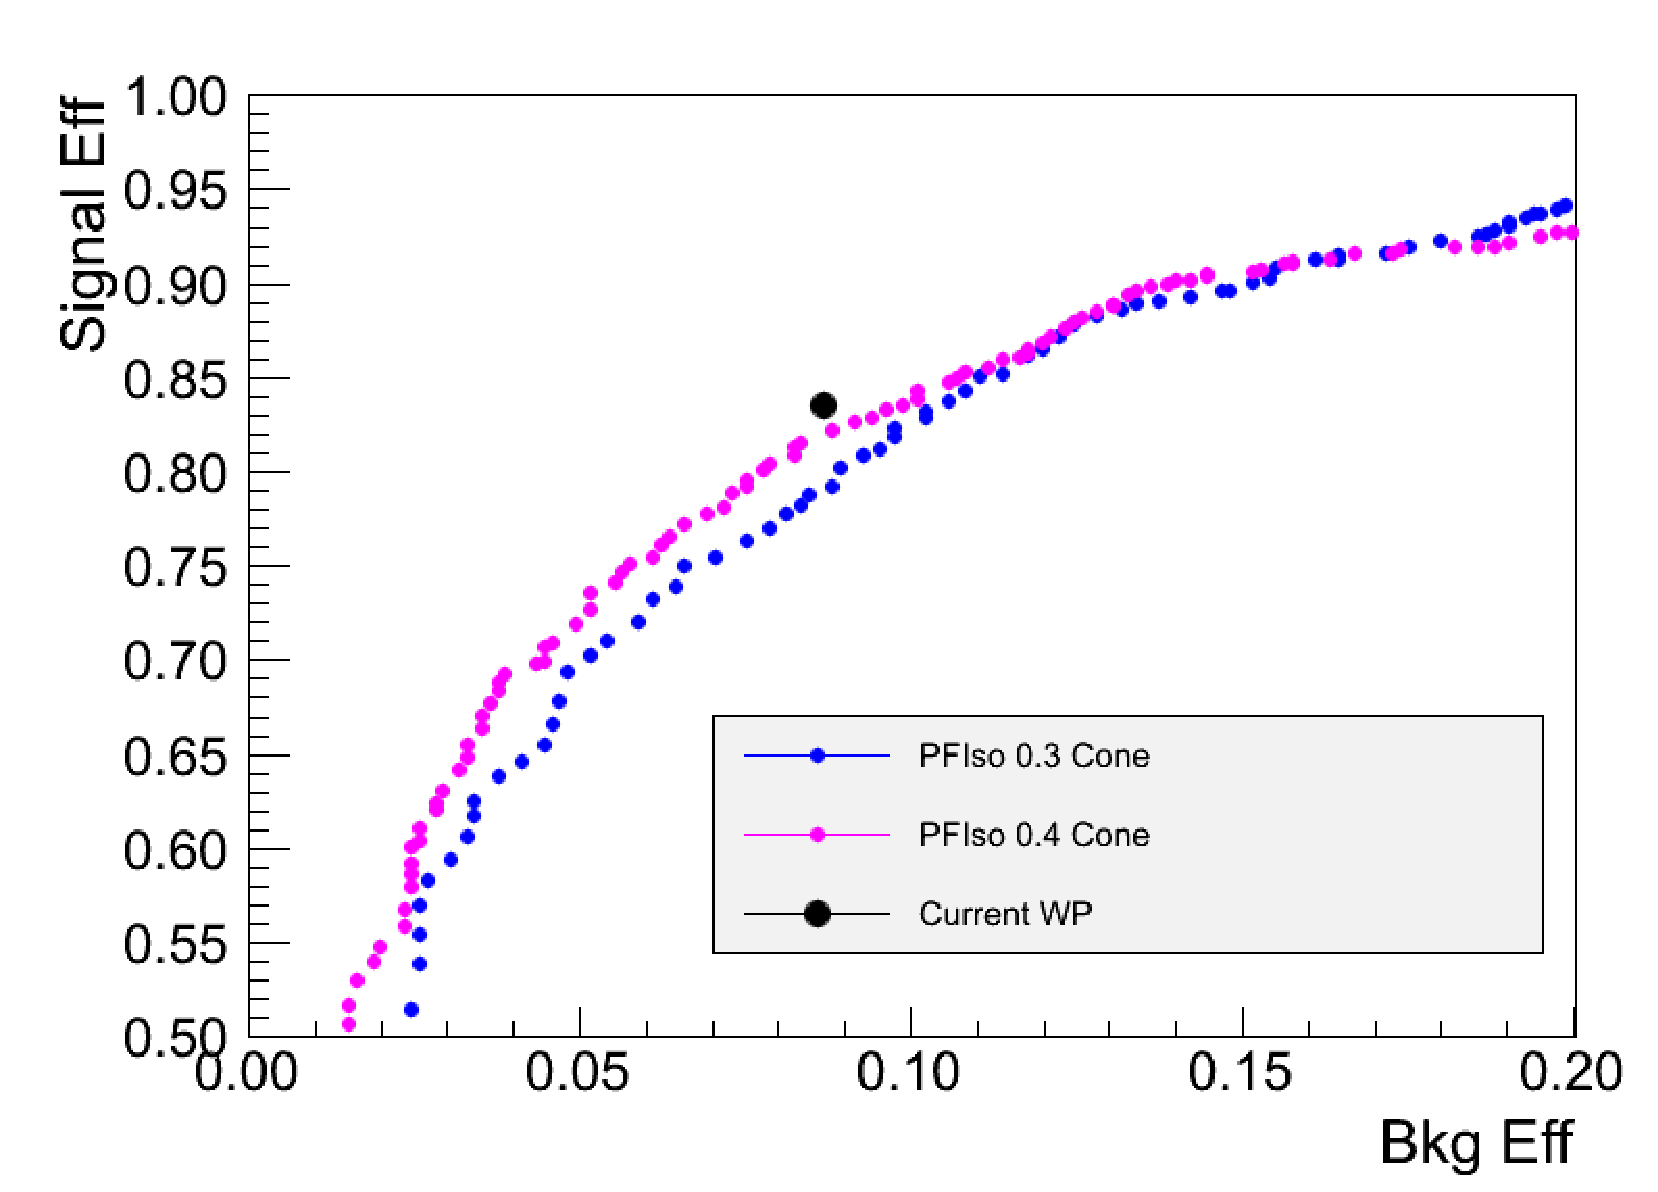
\includegraphics[width=0.45\textwidth]{figures/IsoPerformance_EleBarrel_PFConesize_Pt10To15.pdf}}
\subfigure[$p_{T}$ in $(20,30)$ GeV]{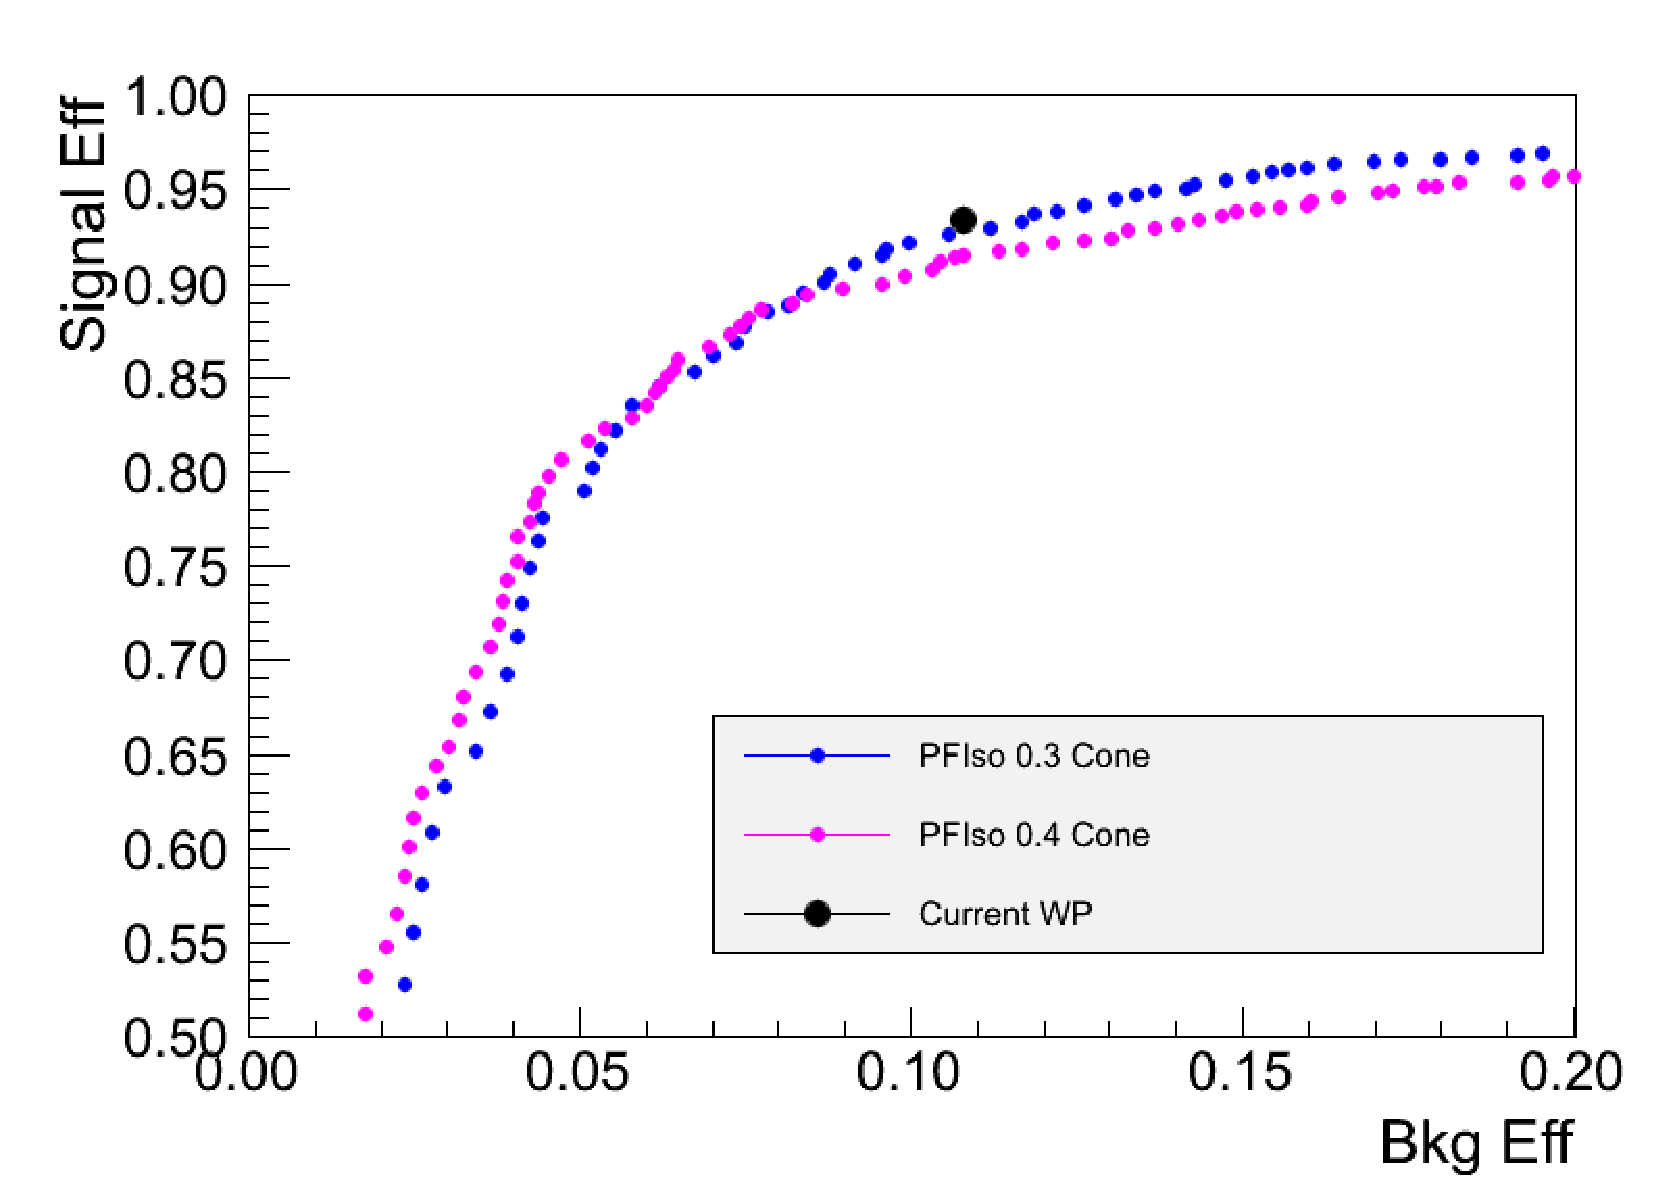
\includegraphics[width=0.45\textwidth]{figures/IsoPerformance_EleBarrel_PFConesize_Pt20To30.pdf}}
\caption{Signal efficiency (HWW130) vs background efficiency for barrel electrons separated into 
low and high $p_{T}$ bins, comparing different isolation cone sizes. }
\label{fig:IsoPerformance_Ele_PFIso_ConeSize}
\end{center}
\end{figure}


\subsubsection{Eta Strip Veto}

Due to the large amount of material that an electron must traverse before reaching the 
electromagnetic calorimeter, there is a large probability for one or multiple
bremstrahlung. Photons from bremstrahlung can also give secondary electrons and positrons
from conversion. As a result, a typical electron will leave an energy footprint within a 
narrow strip in $\eta$, but spread out in $\phi$ as the electron trajectory bends under
the influence of the solenoidal magnetic field. In the standard isolation is has been shown 
that excluding a small strip in eta ($\Delta\eta < 0.025$) in the isolation sum can yield 
better performance for signal to background discrimination. 

The particle flow reconstruction should in principle account for all such bremstrahlung 
and conversions by collecting all such energy clusters and tracks into the electron
object. We investigate the performance difference in using such an eta strip exclusion 
region for the particle flow isolation. 


In Figure \ref{fig:IsoPerformance_Electron_PFIso_VetoStripChoices_Barrel},
and \ref{fig:IsoPerformance_Electron_PFIso_VetoStripChoices_Endcap} we show the
performance curves comparing the case where we impose no $\eta$-strip exclusion,
where we exclude only particle flow photons in the $\eta$-strip and where we
exclude particle flow photons and particle flow electrons in the $\eta$-strip,
for barrel and endcap electrons respectively. We observe that the  $\eta$-strip
exclusion does not change the performance for barrel electrons, suggesting that
the particle flow algorithms to collect all bremstrahlung and conversions
are performing appropriately. In the endcap, however, we observe that performing
the $\eta$-strip exclusion increases the performance, and is much more 
significant at low $p_{T}$. This suggests that there is maybe some 
possibility for improvement, perhaps expected with CMSSW 4\_2\_X. For simplicity,
in the remaining discussion, we will perform the $\eta$-strip exclusion for barrel
and endcap. 

 \begin{figure}[!htbp]
\begin{center}
\subfigure[$p_{T}$ in $(10,15)$ GeV]{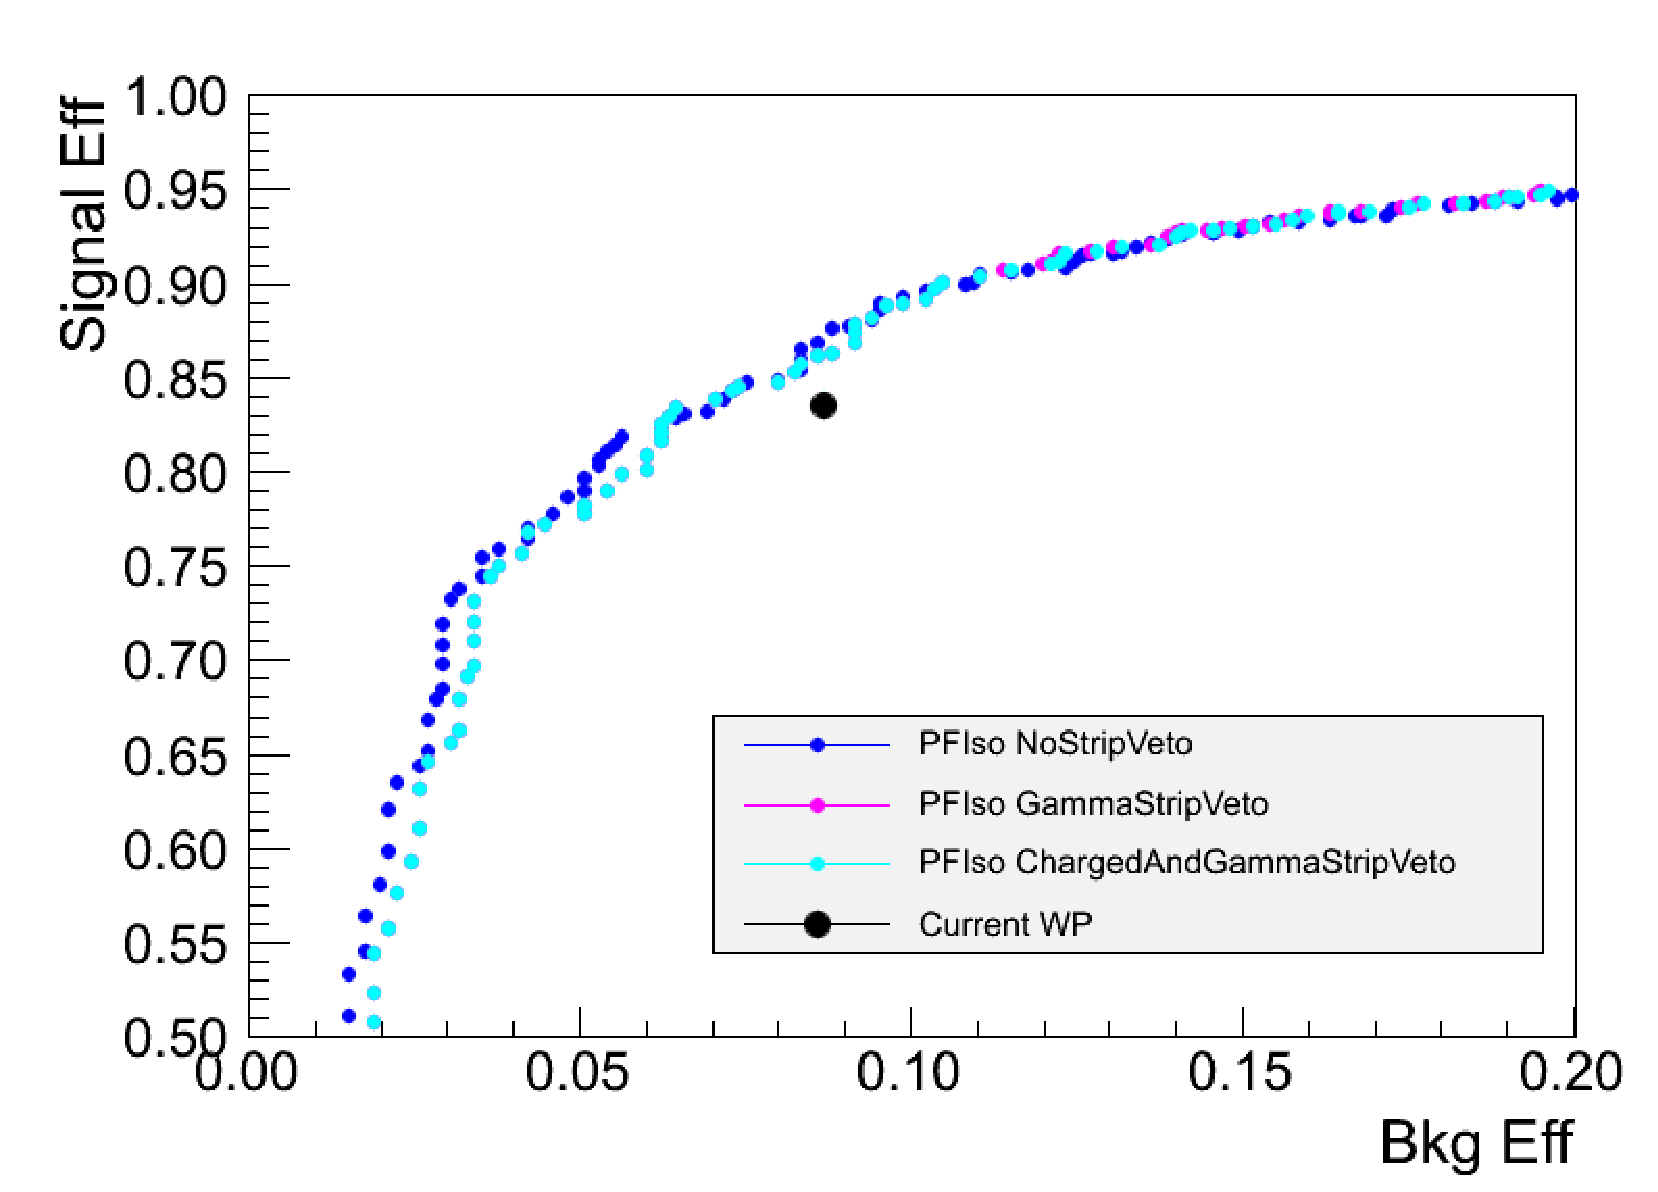
\includegraphics[width=0.48\textwidth]{figures/IsoPerformance_EleBarrel_VetoStripChoices_Pt10To15.pdf}}
\subfigure[$p_{T}$ in $(20,30)$ GeV]{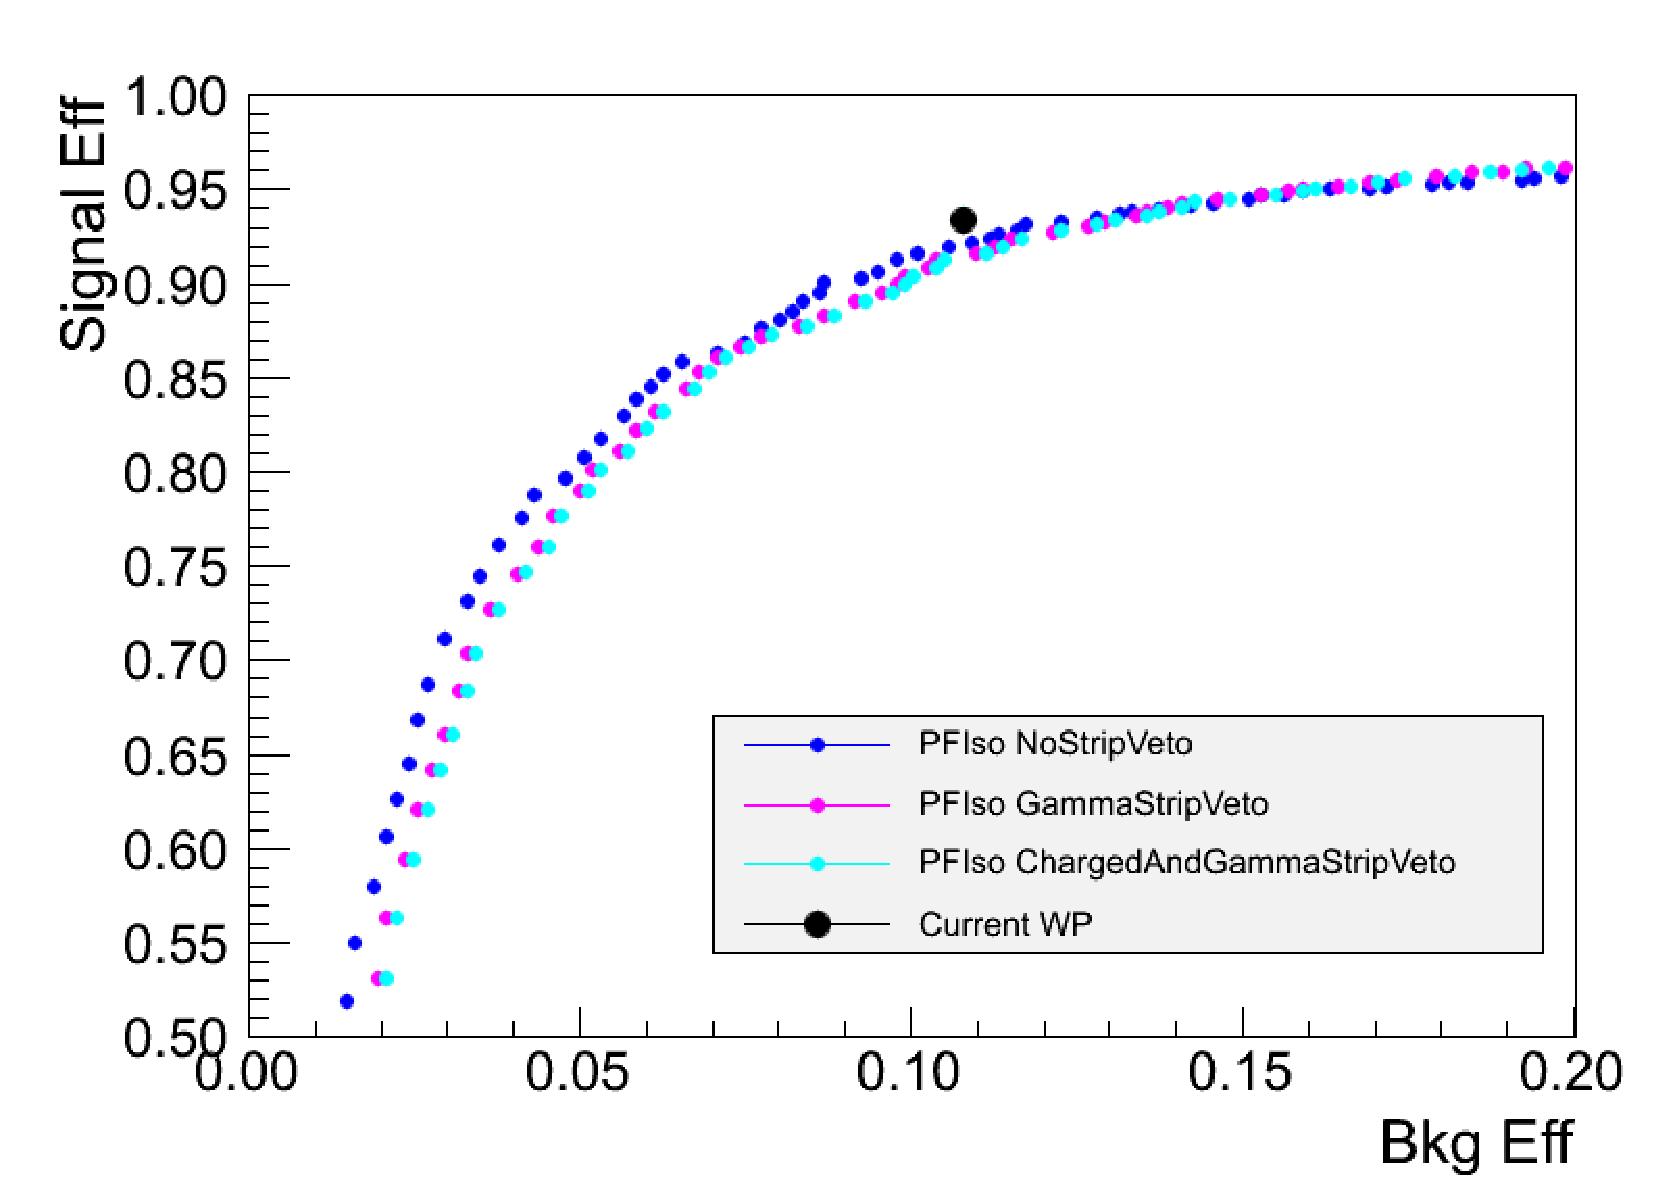
\includegraphics[width=0.48\textwidth]{figures/IsoPerformance_EleBarrel_VetoStripChoices_Pt20To30.pdf}}
\caption{Signal efficiency (HWW130) vs background efficiency for barrel electrons separated into 
low and high $p_{T}$ bins, comparing different choices for the $\eta$-strip exclusion region.}
\label{fig:IsoPerformance_Electron_PFIso_VetoStripChoices_Barrel}
\end{center}
\end{figure}

 
\begin{figure}[!htbp]
\begin{center}
\subfigure[$p_{T}$ in $(10,15)$ GeV]{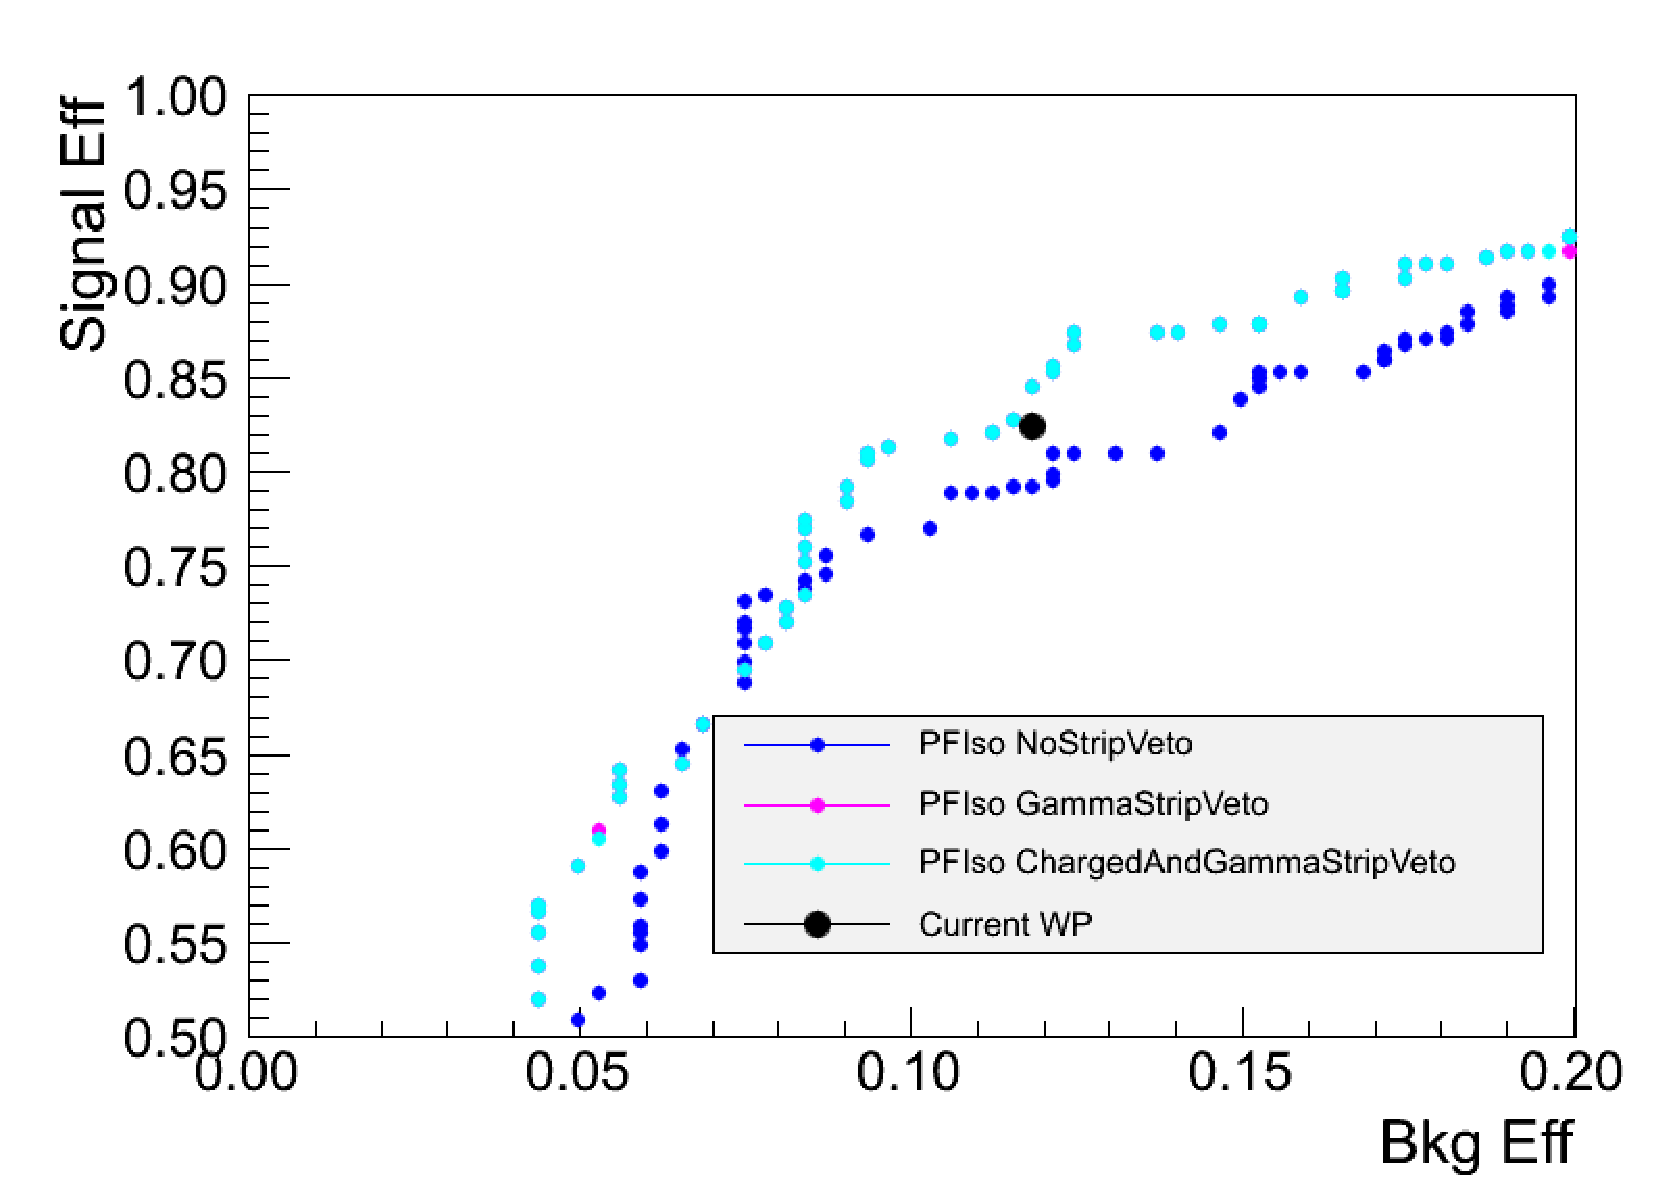
\includegraphics[width=0.48\textwidth]{figures/IsoPerformance_EleEndcap_VetoStripChoices_Pt10To15.pdf}}
\subfigure[$p_{T}$ in $(20,30)$ GeV]{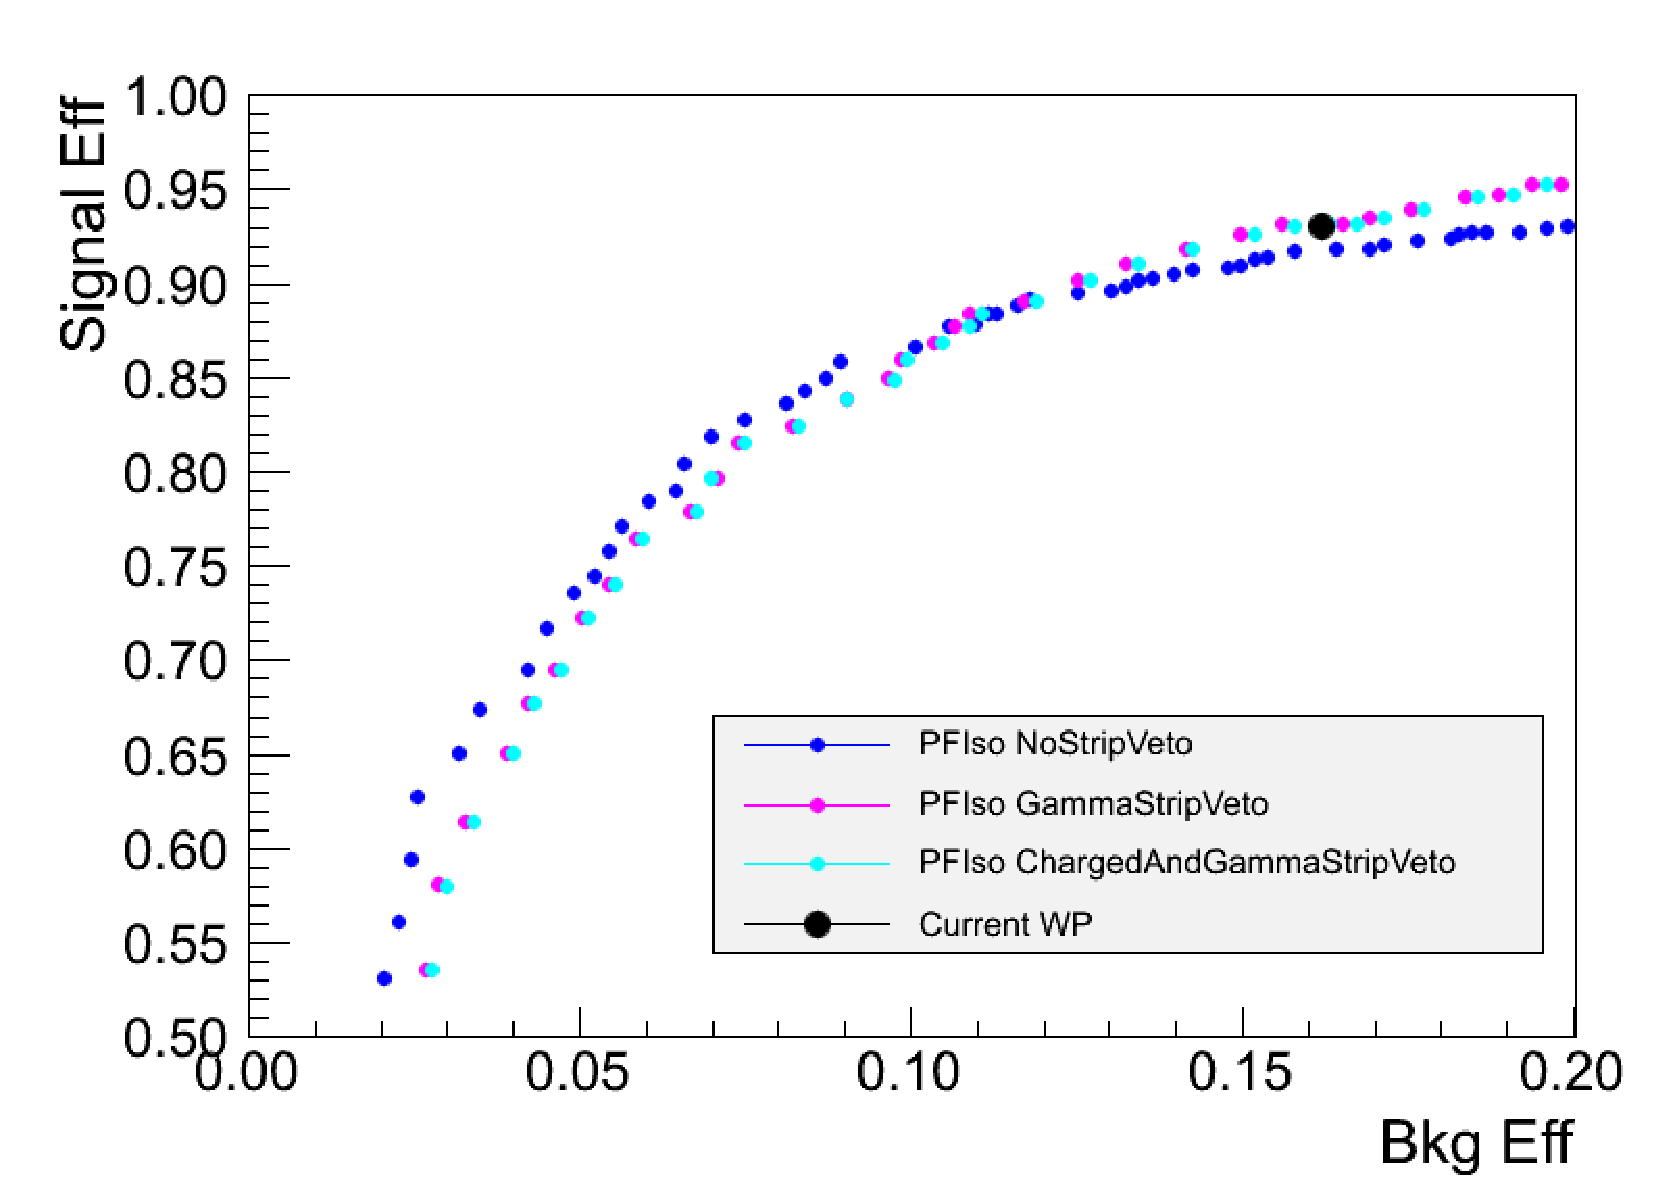
\includegraphics[width=0.48\textwidth]{figures/IsoPerformance_EleEndcap_VetoStripChoices_Pt20To30.pdf}}
\caption{Signal efficiency (HWW130) vs background efficiency for endcap electrons separated into 
low and high $p_{T}$ bins, comparing different choices for the $\eta$-strip exclusion region.}
\label{fig:IsoPerformance_Electron_PFIso_VetoStripChoices_Endcap}
\end{center}
\end{figure}

Finally, we verified that vetoing charged hadrons inside this $\eta$-strip degraded the performance, 
indicating that the particle flow electron reconstruction is not resulting in a significant number
of charged hadrons due to the electron footprint.



\subsubsection{Summary for current pileup scenario}

Having defined the best strategy for the particle flow isolation calculation, we 
compare its performance with the performance of the standard detector based isolation.
Figures \ref{fig:Electron_PFIso_BestLowPU_Barrel} and 
\ref{fig:Electron_PFIso_BestLowPU_Barrel} shows this performance comparison for two 
different cone sizes. 

We observe that for the low $p_{T}$ electrons in the barrel,
there is a large gain in performance using the particle flow isolation with a cone
of $0.4$. For higher $p_{T}$, the performance becomes more similar and a smaller cone size
is preferred. This is most likely due to the particular configuration of the Higgs 
signal, where for higher $p_{T}$ the two leptons are more likely to be near the 
isolation cones of each other. For the endcap, the performance gain of particle flow 
isolation is diminished relative to the barrel. 


\begin{figure}[!htbp]
\begin{center}
\subfigure[$p_{T}$ in $(10,15)$ GeV]{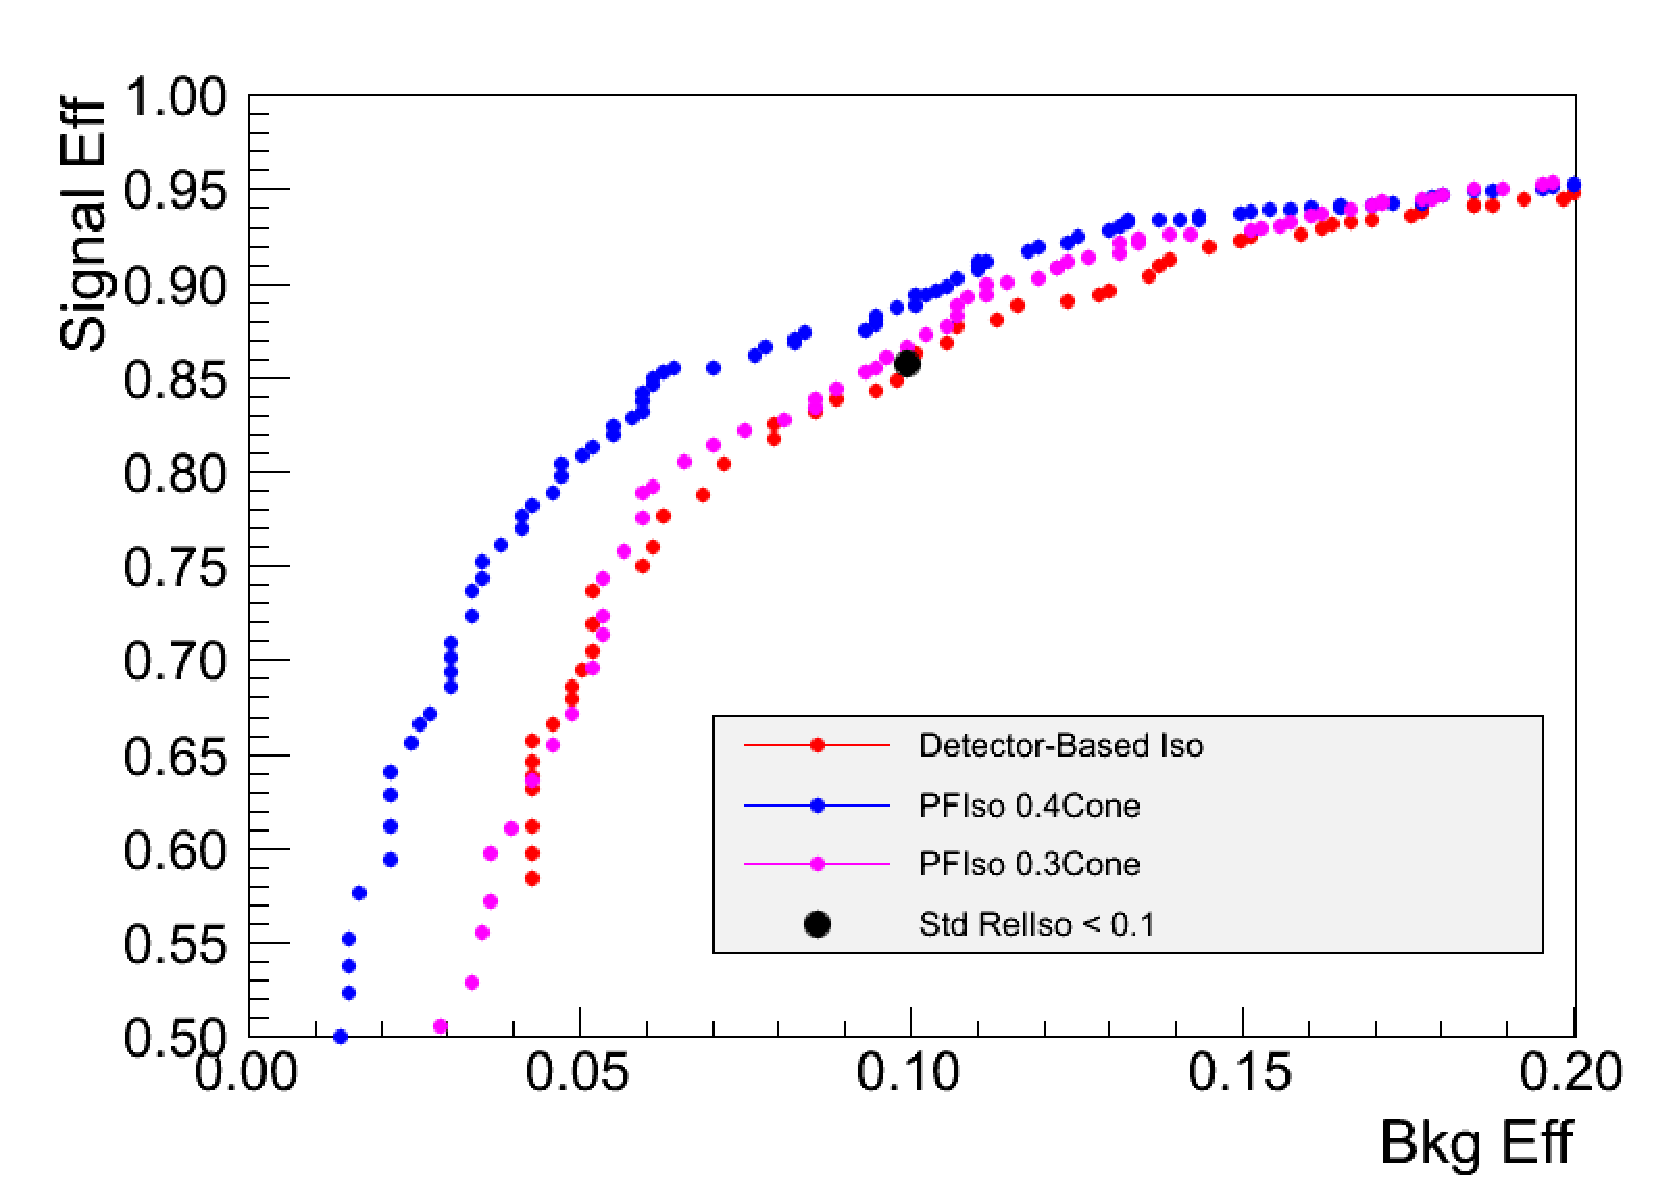
\includegraphics[width=0.48\textwidth]{figures/IsoPerformance_EleBarrel_BestLowPU_Pt10To15.pdf}}
\subfigure[$p_{T}$ in $(20,30)$ GeV]{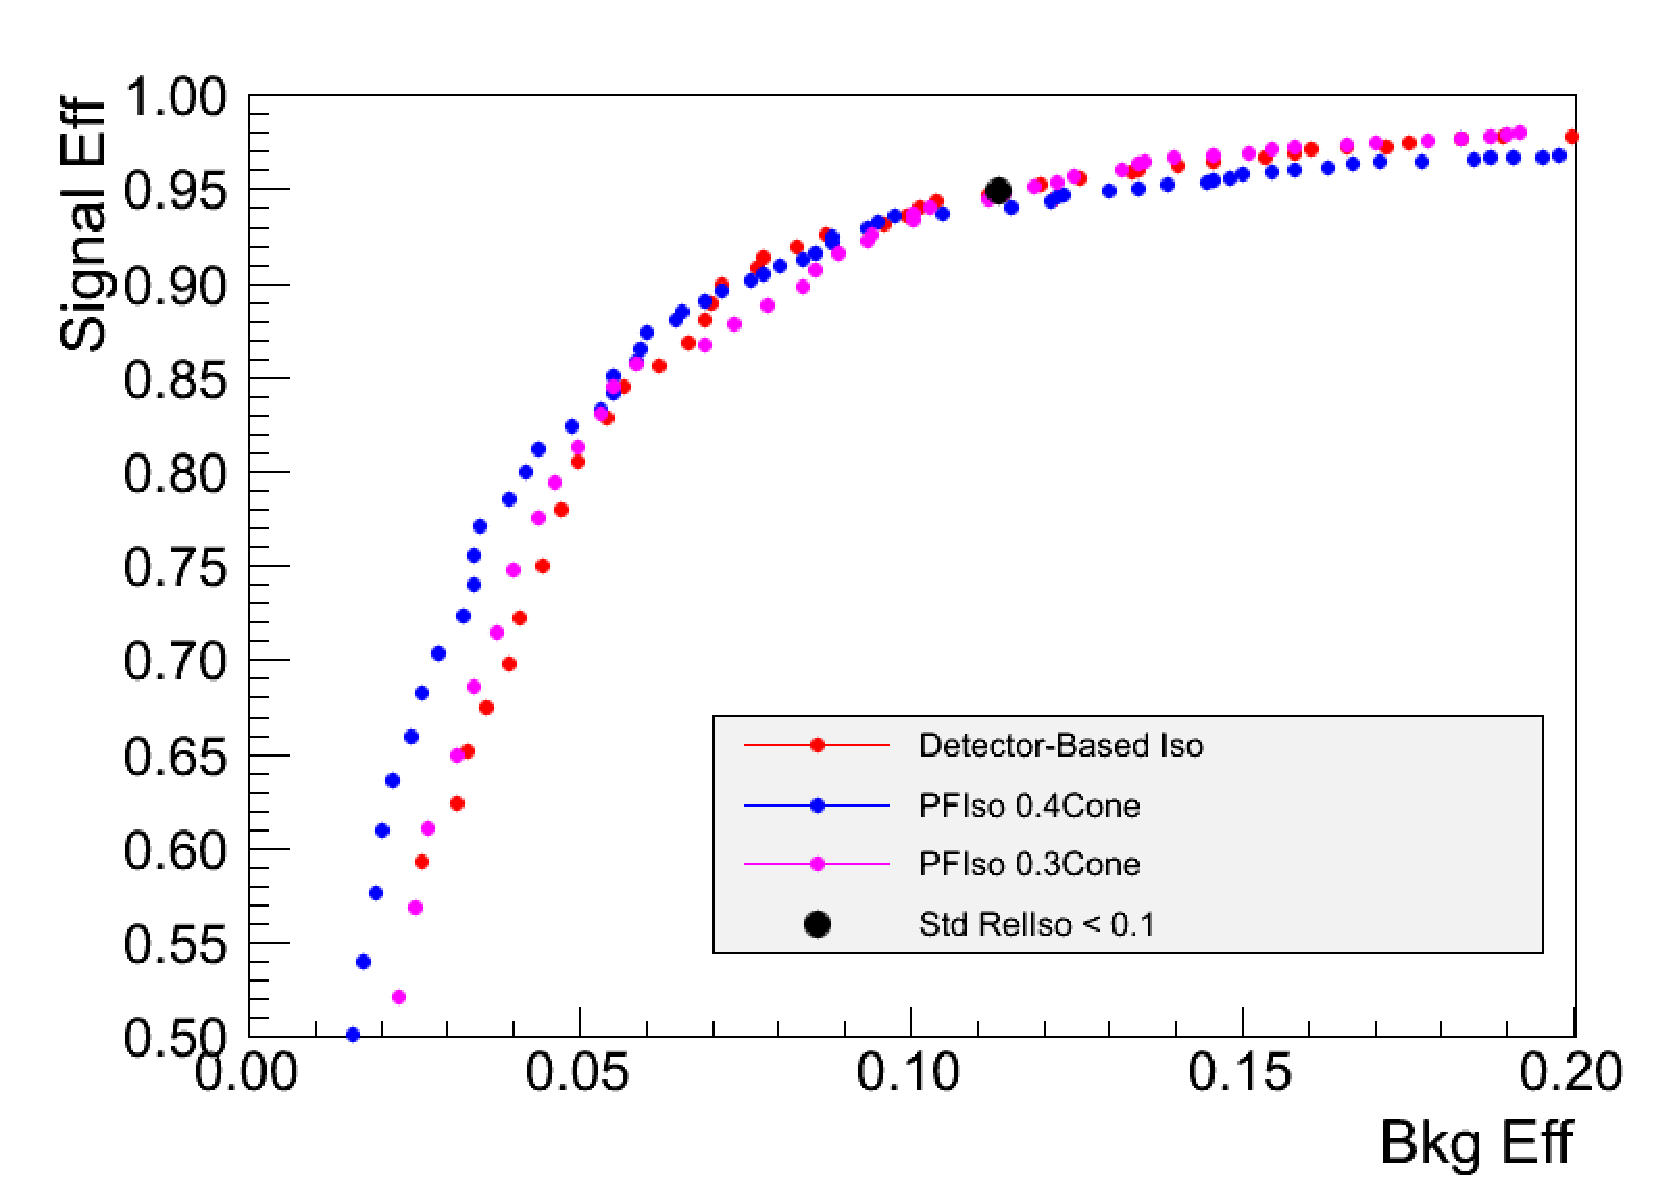
\includegraphics[width=0.48\textwidth]{figures/IsoPerformance_EleBarrel_BestLowPU_Pt20To30.pdf}}
\caption{Signal efficiency (HWW130) vs background efficiency for barrel electrons separated into 
low and high $p_{T}$ bins, comparing the standard detector-based isolation with the best choices 
for particle flow isolation.}
\label{fig:Electron_PFIso_BestLowPU_Barrel}
\end{center}
\end{figure}


\begin{figure}[!htbp]
\begin{center}
\subfigure[$p_{T}$ in $(10,15)$ GeV]{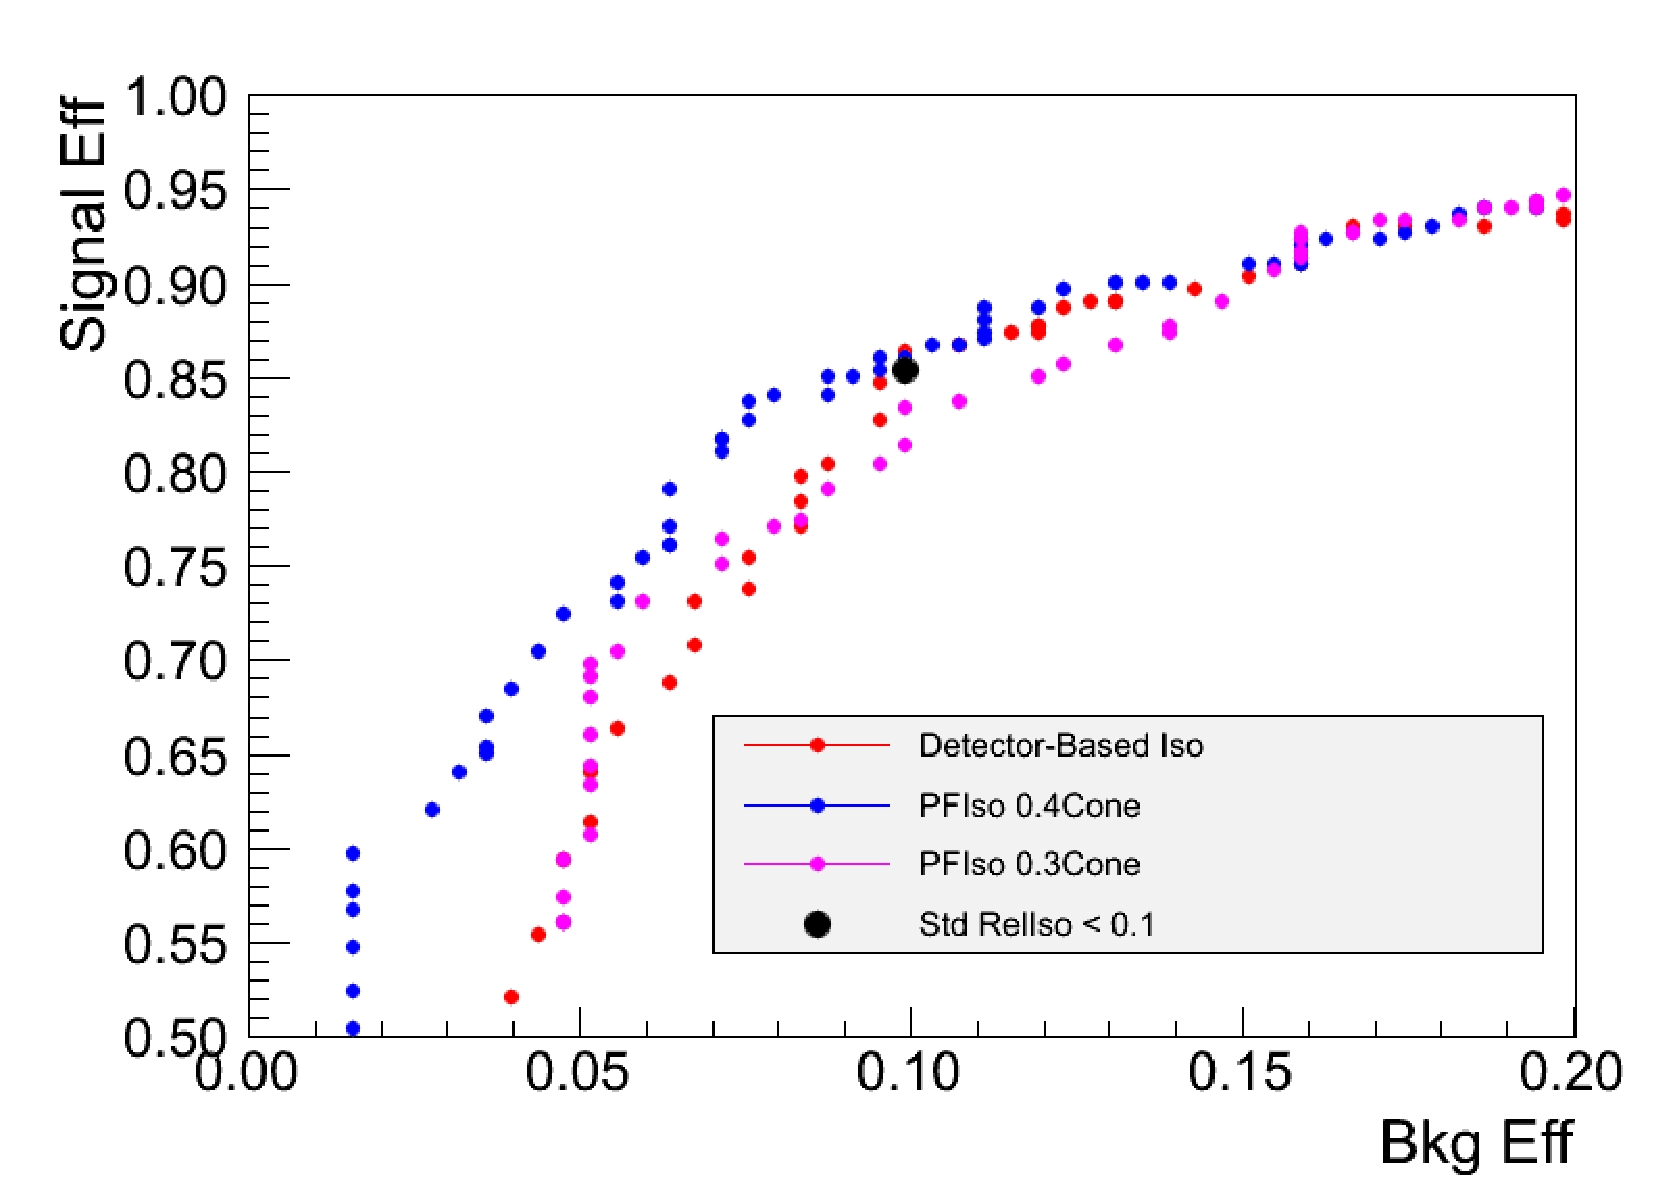
\includegraphics[width=0.48\textwidth]{figures/IsoPerformance_EleEndcap_BestLowPU_Pt10To15.pdf}}
\subfigure[$p_{T}$ in $(20,30)$ GeV]{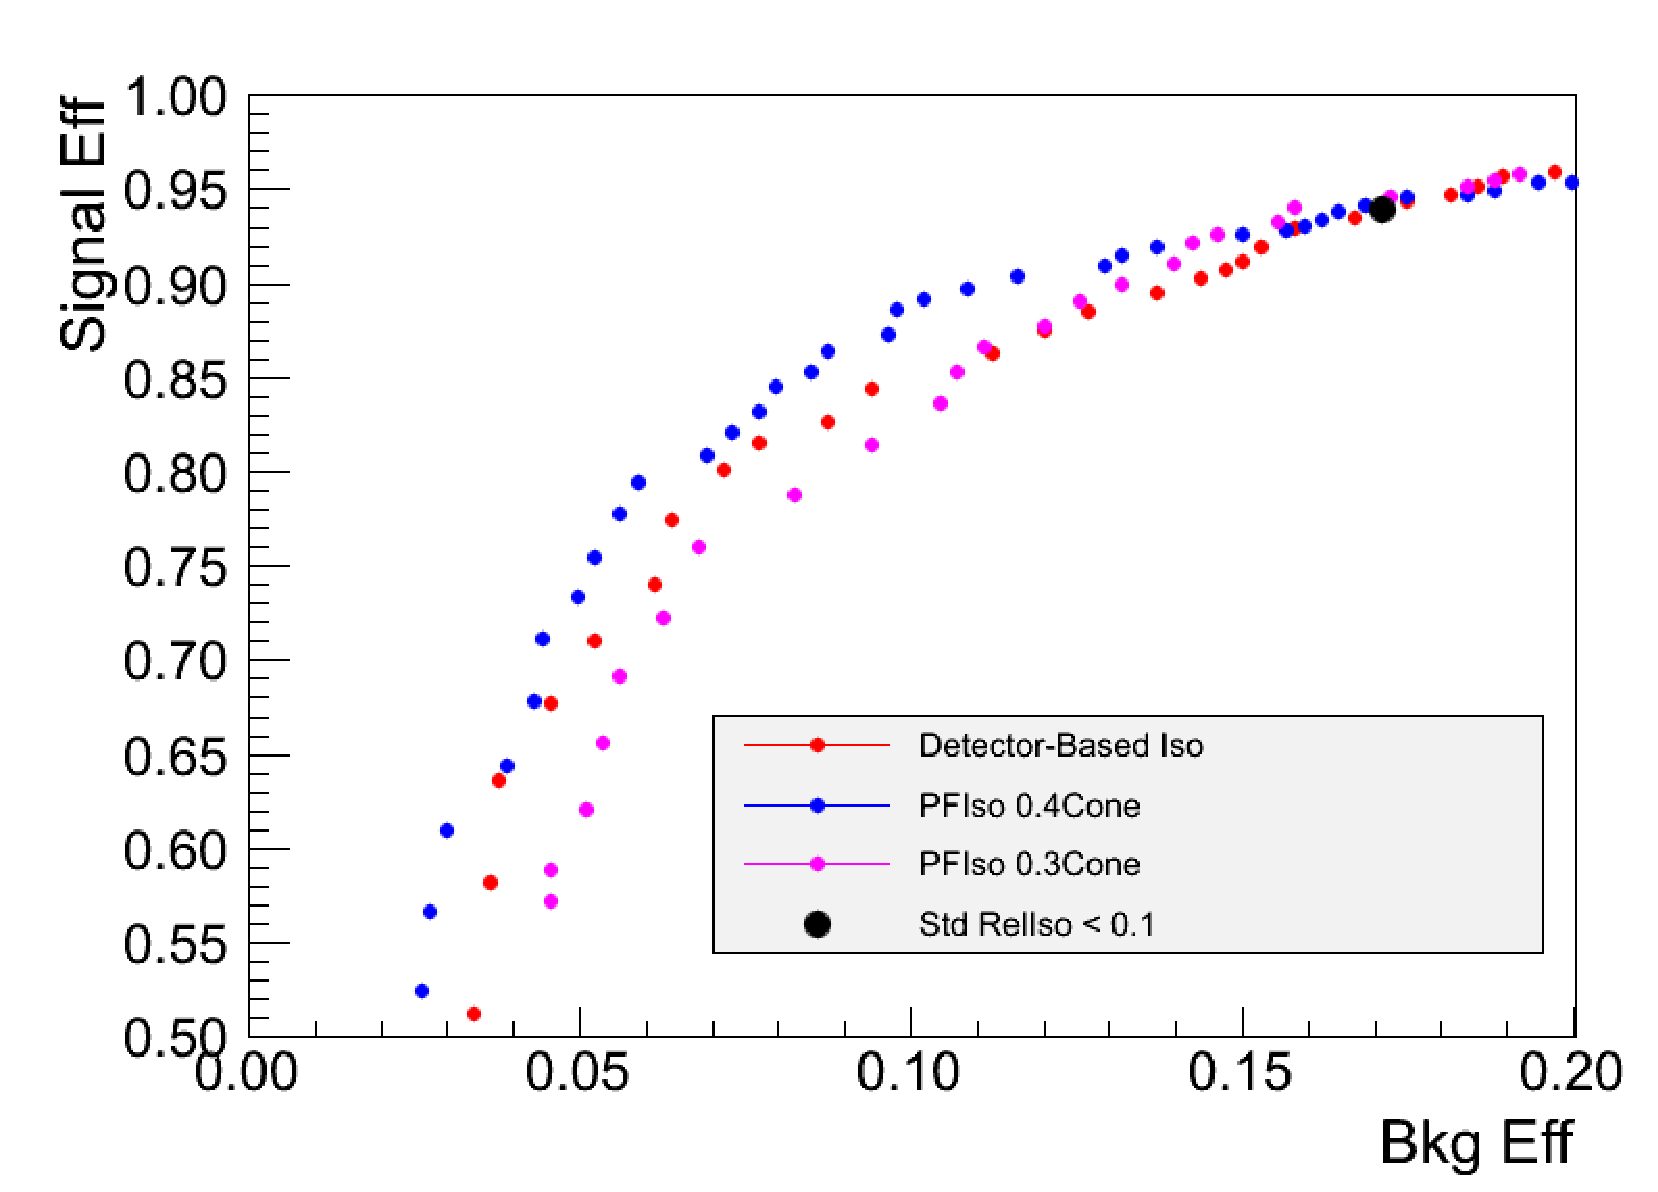
\includegraphics[width=0.48\textwidth]{figures/IsoPerformance_EleEndcap_BestLowPU_Pt20To30.pdf}}
\caption{Signal efficiency (HWW130) vs background efficiency for endcap electrons separated into 
low and high $p_{T}$ bins, comparing the standard detector-based isolation with the best choices 
for particle flow isolation.}
\label{fig:Electron_PFIso_BestLowPU_Endcap}
\end{center}
\end{figure}




\subsection{Effect of pileup}

There have been suggestions that the pileup scenario for the LHC in the 
second half of 2011 will become more severe than what has been faced so far.
Therefore, we study and address various methods to perform corrections
for the lepton isolation calculation. 

First, we characterize the effect of the pileup contribution for the 
scenario faced in the first $200$ \ipb of integrated luminosity.  
Figure \ref{fig:StandardIsoEfficiency_vs_NVertices} shows the 
efficiency of the standard detector based lepton isolation requirement 
as a function of the number of reconstructed vertices for the 
Higgs signal Monte Carlo simulation sample, separately for high 
and low $p_{T}$. We observe that for high $p_{T}$ leptons, there is a 
negligible effect from pileup, while for low $p_{T}$ leptons the 
isolation efficiency decreases by $10\%$ - $20\%$ as the number
of reconstructed vertices increases from one to ten. Averaging 
over the full $p_{T}$ spectrum of the Higgs sample with mass of
$130$ GeV, we find an average loss of efficiency for electrons and
muons of  $3\%$ and $2\%$ respectively. 

\begin{figure}[!htbp]
\begin{center}
\subfigure[Electrons]{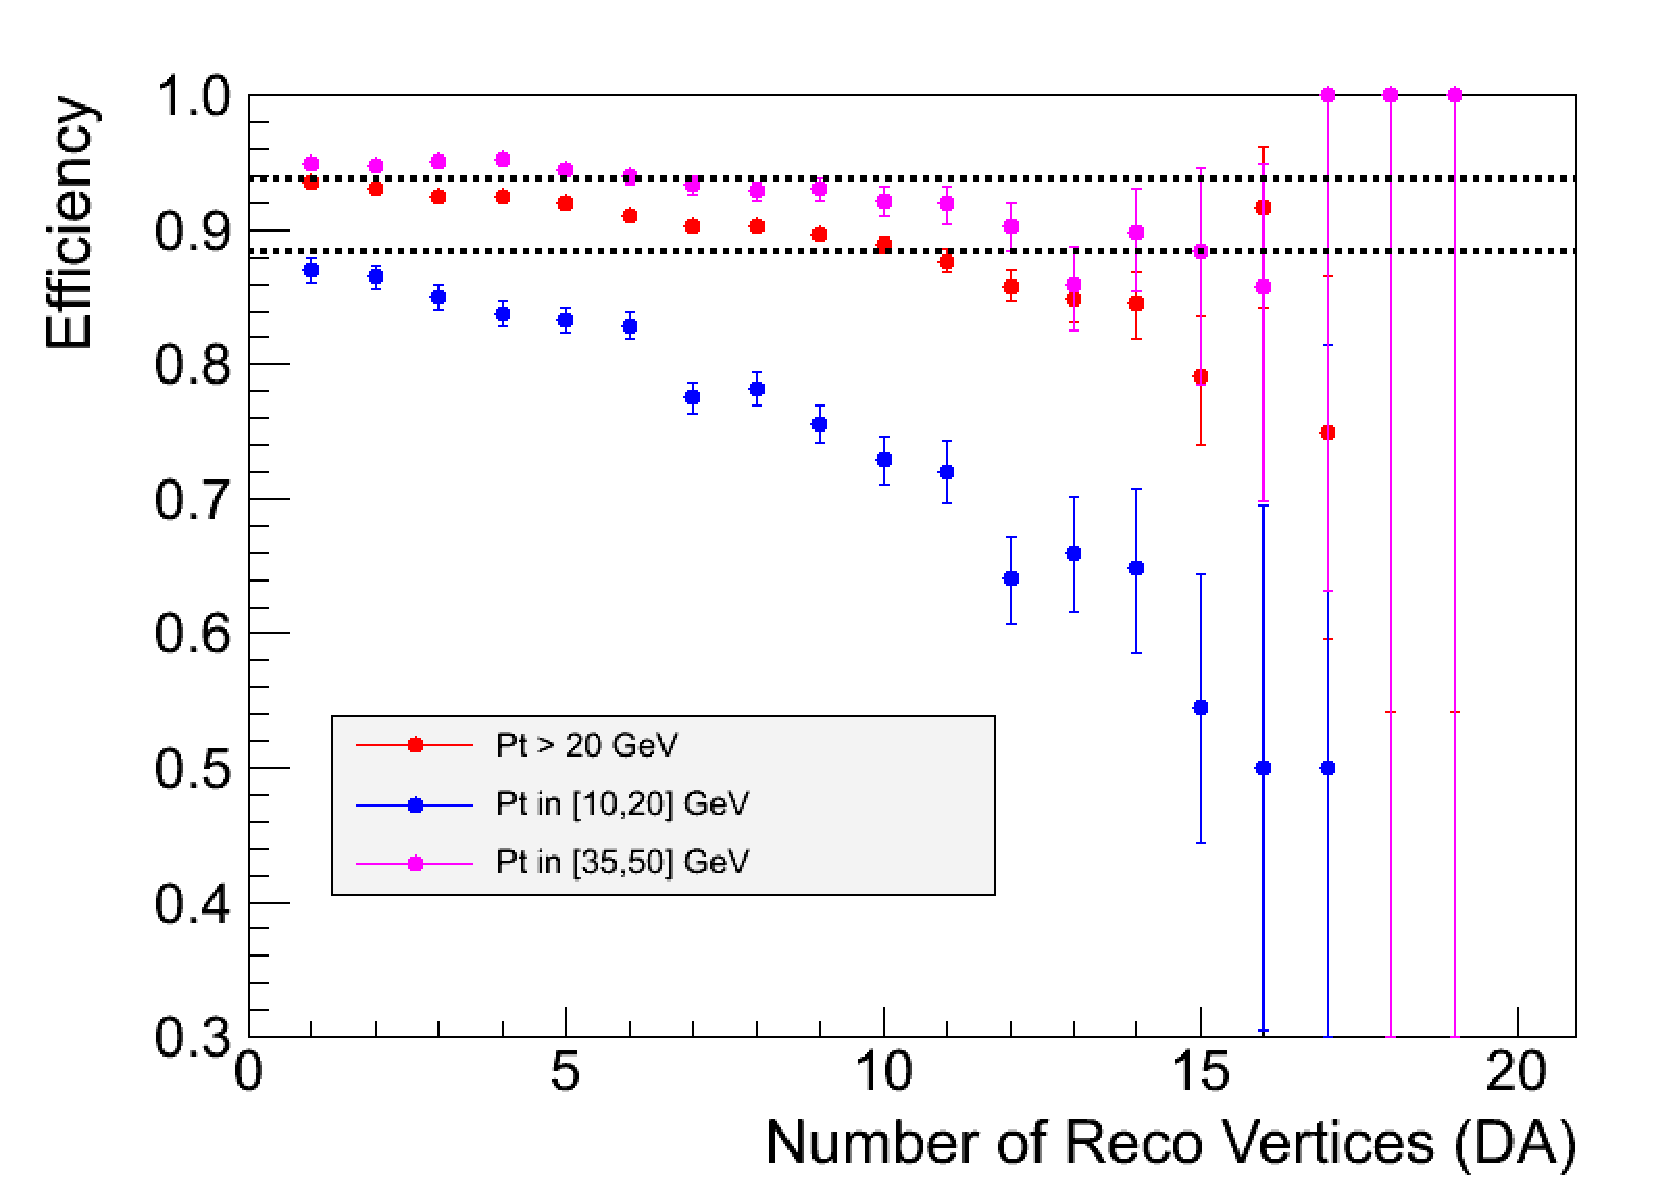
\includegraphics[width=0.48\textwidth]{figures/ElectronIsolationVsNVertices_HWW130.pdf}}
\subfigure[Muons]{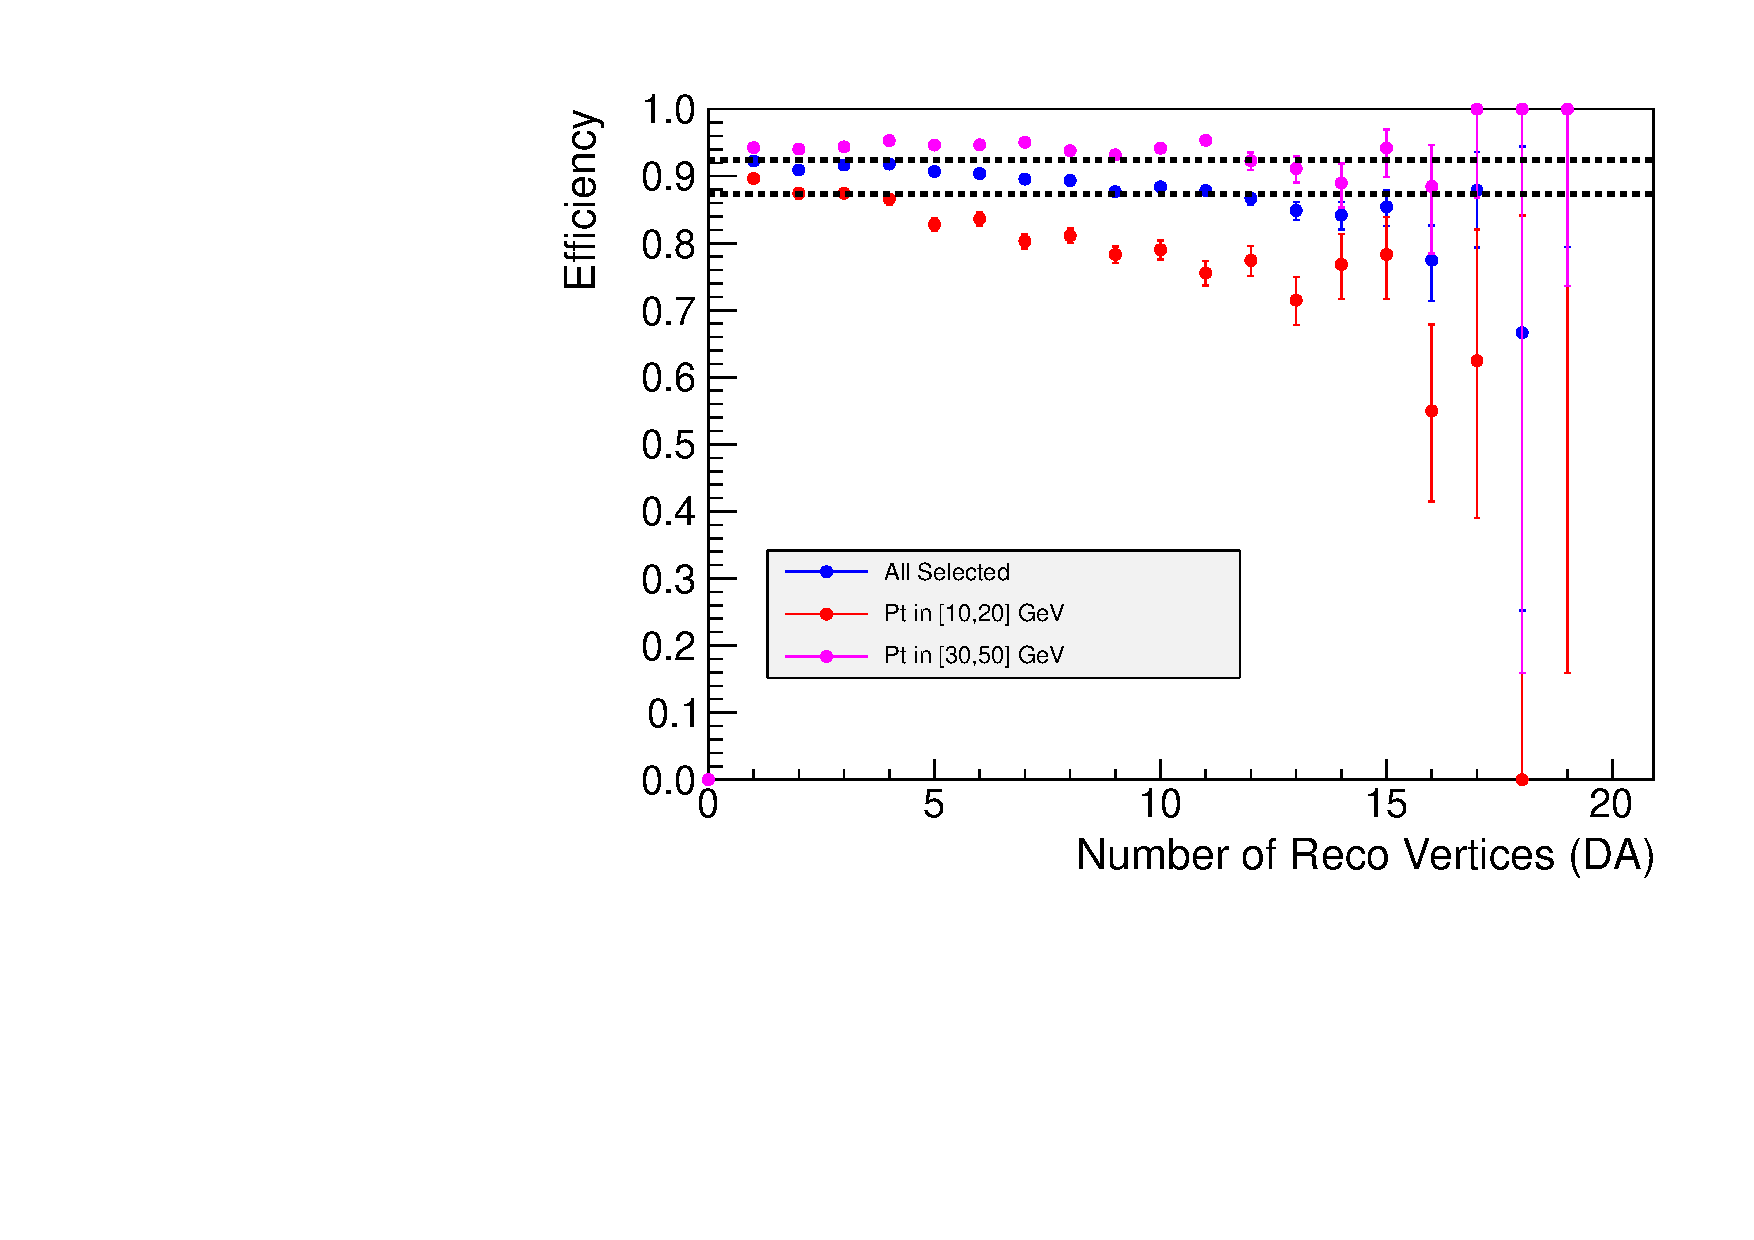
\includegraphics[width=0.48\textwidth]{figures/MuonIsolationVsNVertices_HWW130.pdf}}
\caption{ Isolation efficiency as a function of the number of reconstructed vertices, for electrons and muons using 
the detector based isolation cuts for the HWW130 signal sample. The efficiency is shown separately for
low and high $p_{T}$ leptons.  }
\label{fig:StandardIsoEfficiency_vs_NVertices}
\end{center}
\end{figure}

\begin{table}[!htbp]
\begin{center}
\begin{tabular}{|l|c|c|c|}
\hline
	Lepton & No Pileup & Average Pileup & Efficiency Loss due to pileup\\
\hline
Electron (relative iso $< 0.10$) &  $92.4\%$ & $89.7\%$ & $2.9\%$ \\
Muon (relative iso $< 0.15$)    &  $92.3\%$ & $90.2\%$ & $2.3\%$ \\
\hline
\end{tabular}
\caption{Lepton isolation efficiencies at low and high pileup conditions with the standard
detector based isolation cuts. }
\label{tab:LeptonIsolationEfficiencyLossFromPileup}
\end{center}
\end{table}


\subsection{High pileup}

We study the performance of a number of different schemes for treating pileup,
for a high pileup scenario with the number of reconstructed vertices between 
$7$ and $15$. 

The first handle to address pileup subtraction to apply a cut in $\Delta$z for 
charged particles. Figure \ref{fig:IsoPerformance_EleBarrel_dZCut} shows the difference
in performance between rejecting charged particles inside the isolation cone 
incompatible with the primary vertex and not rejecting them. There is a clear increase
in performance if one requires this rejection.

\begin{figure}[!htbp]
\begin{center}
\subfigure[NVtx: 3-6]{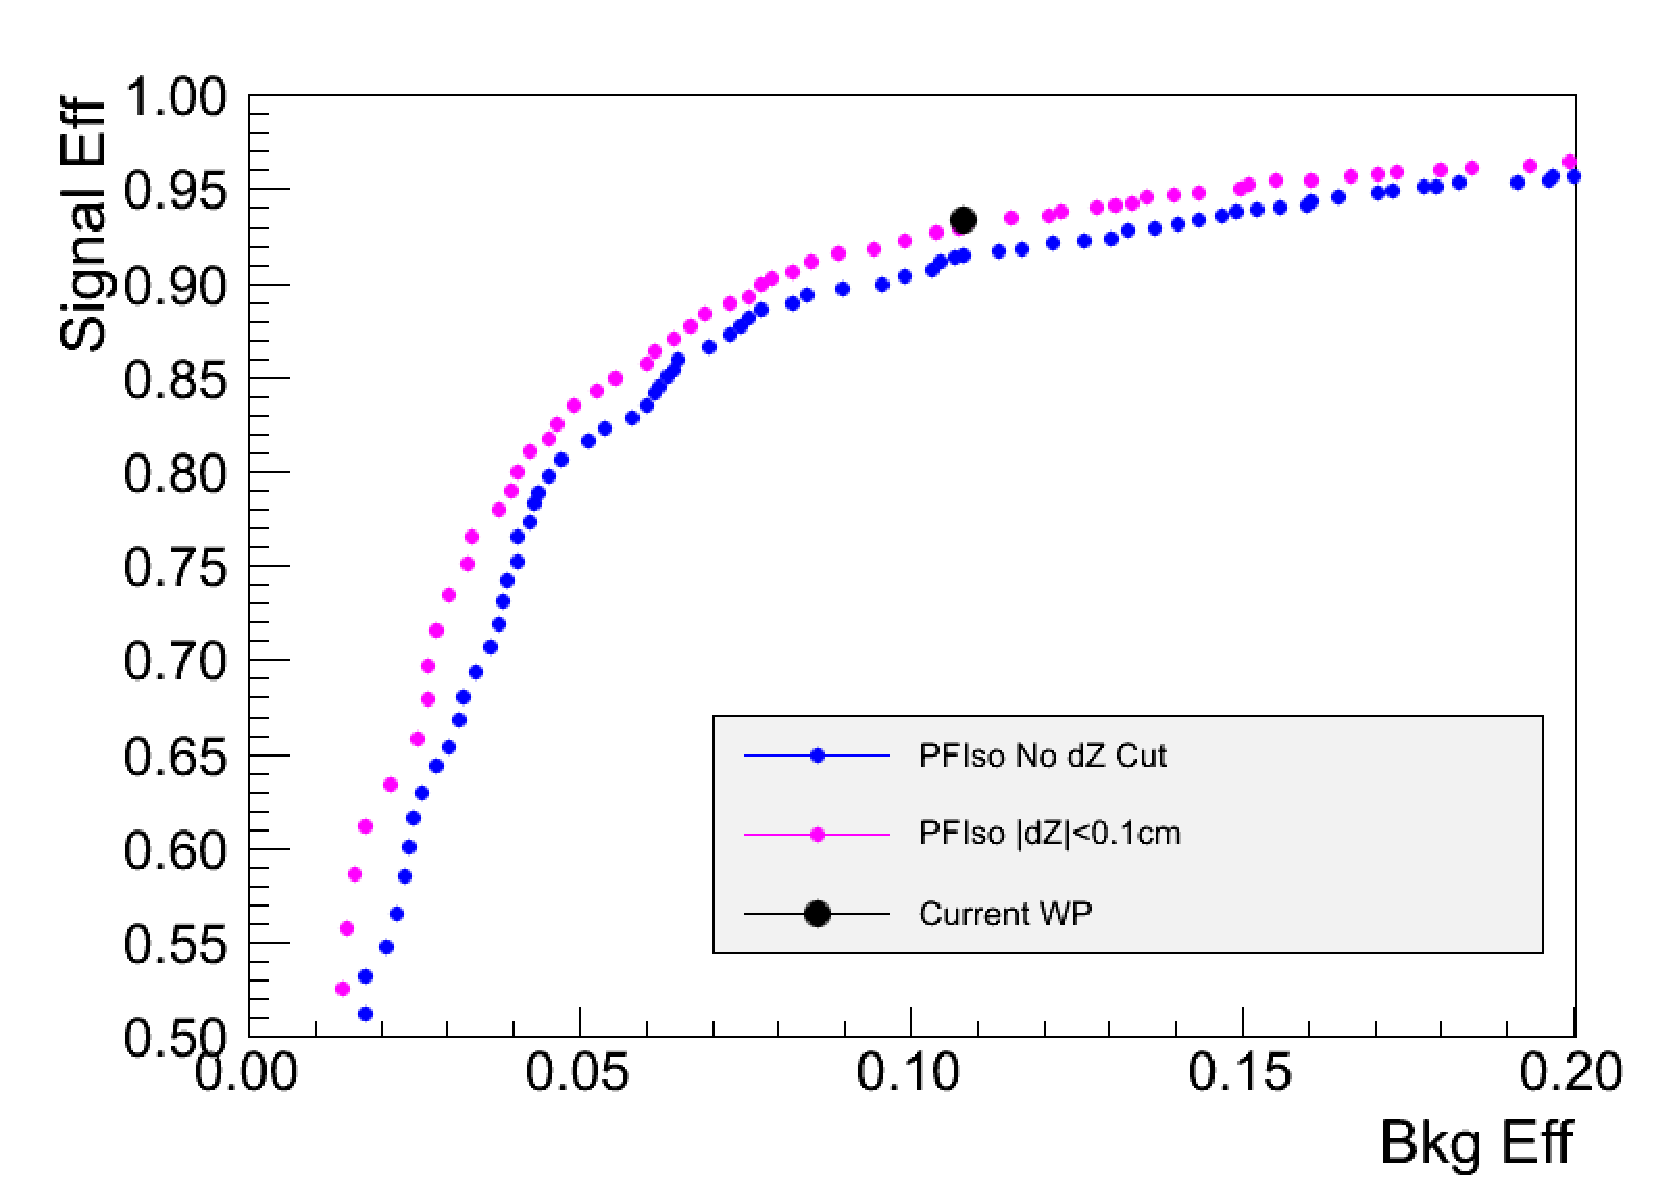
\includegraphics[width=0.48\textwidth]{figures/IsoPerformance_EleBarrel_NVtx3to6_dZCut_Pt20To30.pdf}}
\subfigure[NVtx: 7-15]{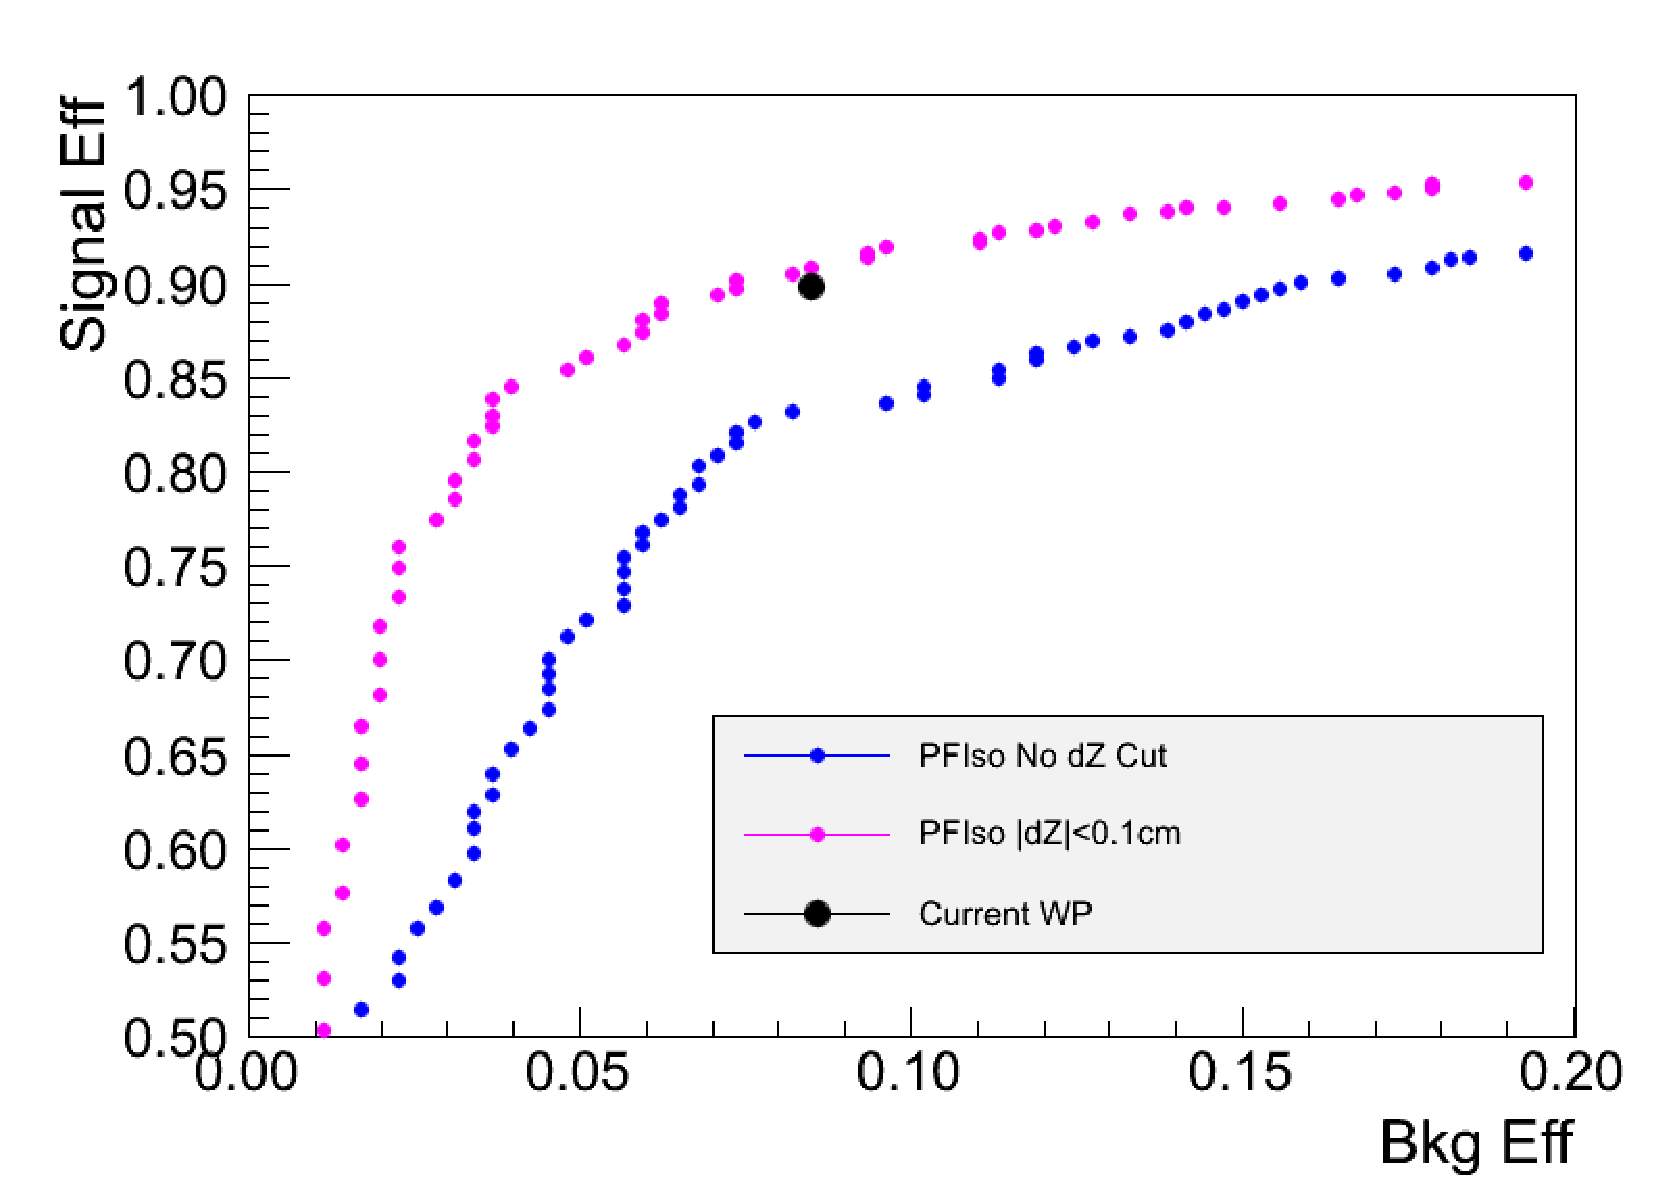
\includegraphics[width=0.48\textwidth]{figures/IsoPerformance_EleBarrel_NVtx7to15_dZCut_Pt20To30.pdf}}
\caption{ Signal efficiency (HWW130) vs background efficiency for barrel electrons separated into 
low and high pileup, comparing with and without the $\Delta$z requirement for charged particles.
Electrons with $p_{T} > 20$ GeV are used. }
\label{fig:IsoPerformance_EleBarrel_dZCut}
\end{center}
\end{figure}


Having rejected charged particles from pileup interactions in the isolation cone, there are
a couple of ways to reject neutral particles from pileup. One scheme is to perform a 
subtraction of energy inside the isolation cone due to pileup based on the average energy
density in the event. We first compute the average energy density, $\rho_{\mathrm{FJ}}$ due to 
pileup using the Fast Jet procedure, plot the mean of $\rho_{\mathrm{FJ}}$ as a function of
the number of reconstructed vertices, and finally perform a linear fit. Next we perform the 
same linear fit in the mean of the relevant isolation variable as a function of the number of 
reconstructed vertices, and then define the effective area as 
$\mathrm{EA} = \mathrm{slope}_{\rho} / \mathrm{slope}_{\mathrm{iso}}$. This effective area 
is multiplied by the $\rho$ for every event to obtain the contamination of pileup energy
inside the isolation cone. This energy contamination is subtracted from the lepton isolation
to correct for pileup. Figure \ref{fig:IsoPerformance_EleBarrel_EffectiveAreaCorrection}
compares the performance of the standard isolation and the particle flow isolation with and
without the effective area corrections. We observe that there is essentially no change
in the performance after performing the correction procedure described above.

\begin{figure}[!htbp]
\begin{center}
\subfigure[$p_{T}$ in $(10,15)$ GeV]{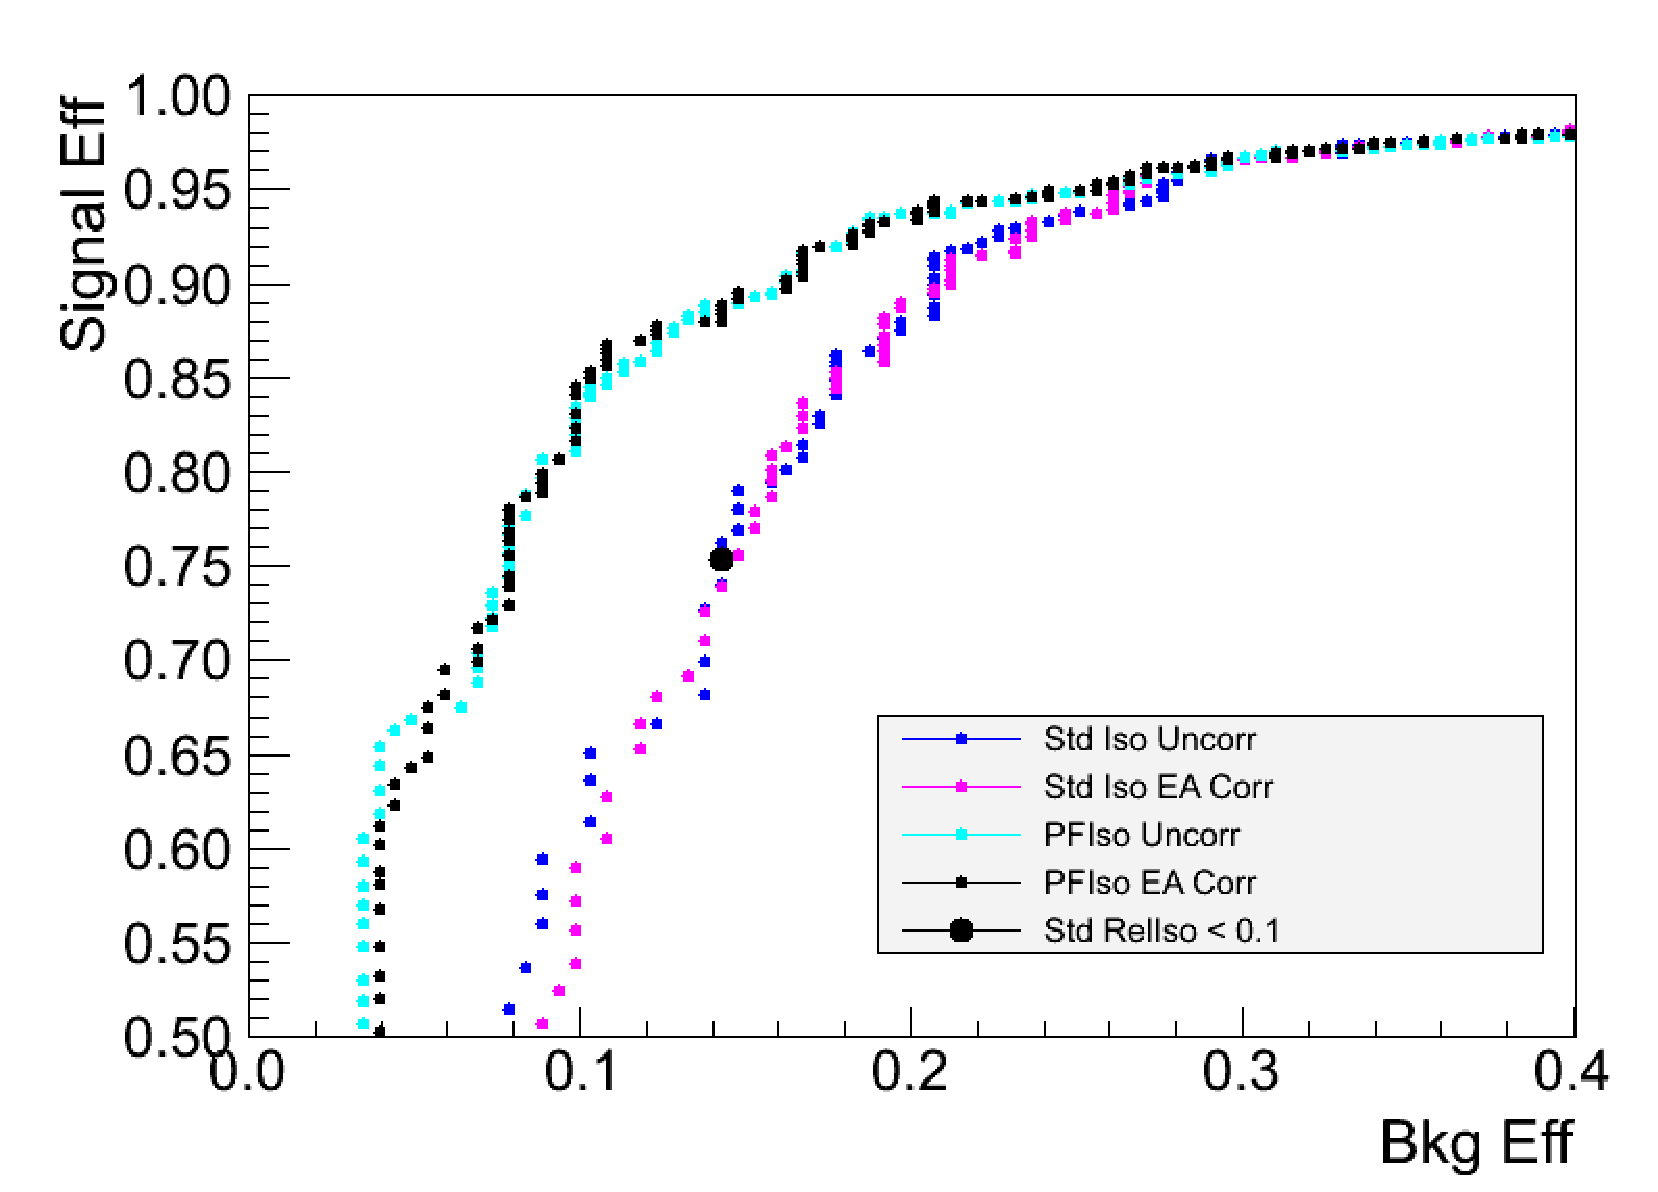
\includegraphics[width=0.48\textwidth]{figures/IsoPerformance_EleBarrel_EACorr_NVtx7To15_Pt10To15.pdf}}
\subfigure[$p_{T}$ in $(20,30)$ GeV]{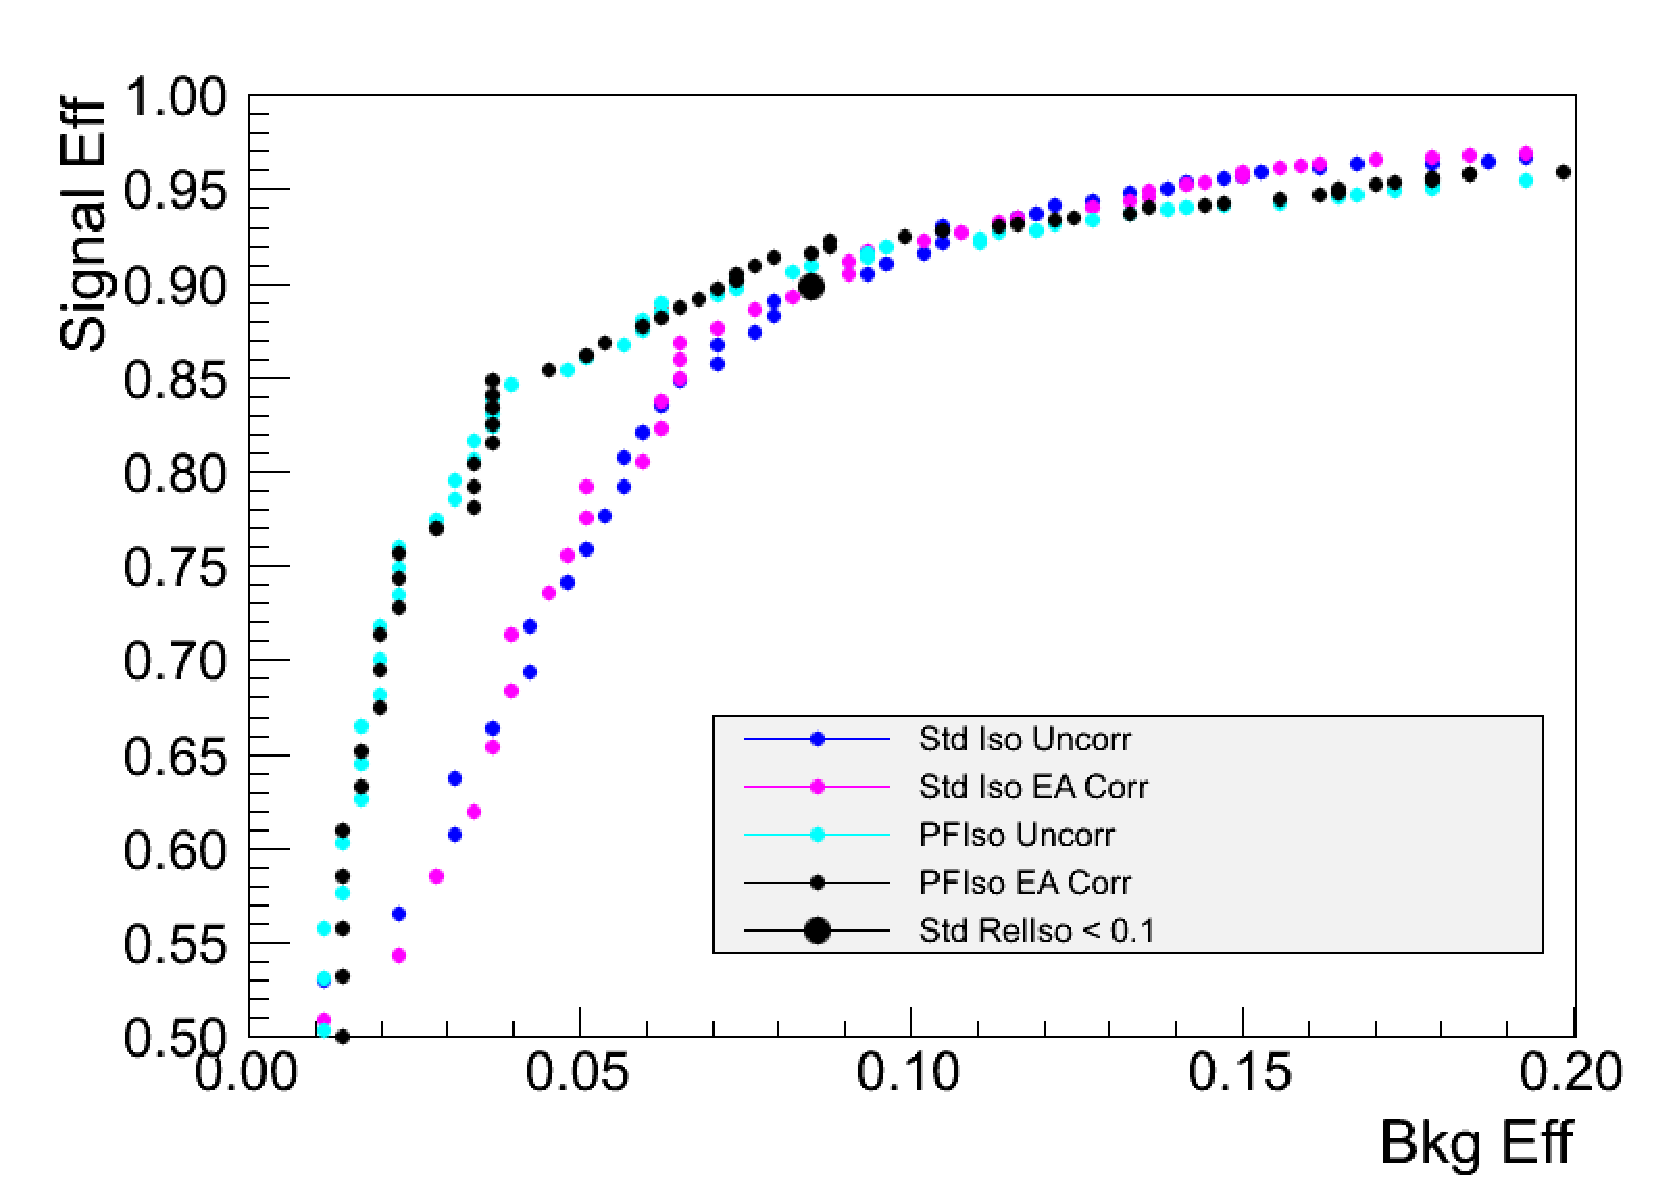
\includegraphics[width=0.48\textwidth]{figures/IsoPerformance_EleBarrel_EACorr_NVtx7To15_Pt20To30.pdf}}
\caption{Signal efficiency (HWW130) vs background efficiency for barrel electrons separated into 
low and high $p_{T}$ bins, comparing the effect of applying the effective area pileup correction.
The high pileup scenario (NVtx $7$-$15$) is shown.}
\label{fig:IsoPerformance_EleBarrel_EffectiveAreaCorrection}
\end{center}
\end{figure}

An alternative scheme for addressing pileup is to increase the $p_{T}$ threshold on neutral 
particles inside the isolation cone. Since particles produced in typical pileup events are
fairly low in $p_{T}$, this decreases sensitivity of the isolation cut to the presence of 
pileup. In Figure \ref{fig:IsoPerformance_Ele_PtThresholds}, we compare the performance
of the particle flow isolation cut, varying the $p_{T}$ threshold for neutral particles
inside the isolation cone. We observe a fairly small degradation in performance going up
to a threshold of $1.0$ GeV. In the endcap, the degradation in performance is a bit
larger. 

\begin{figure}[!htbp]
\begin{center}
\subfigure[Barrel]{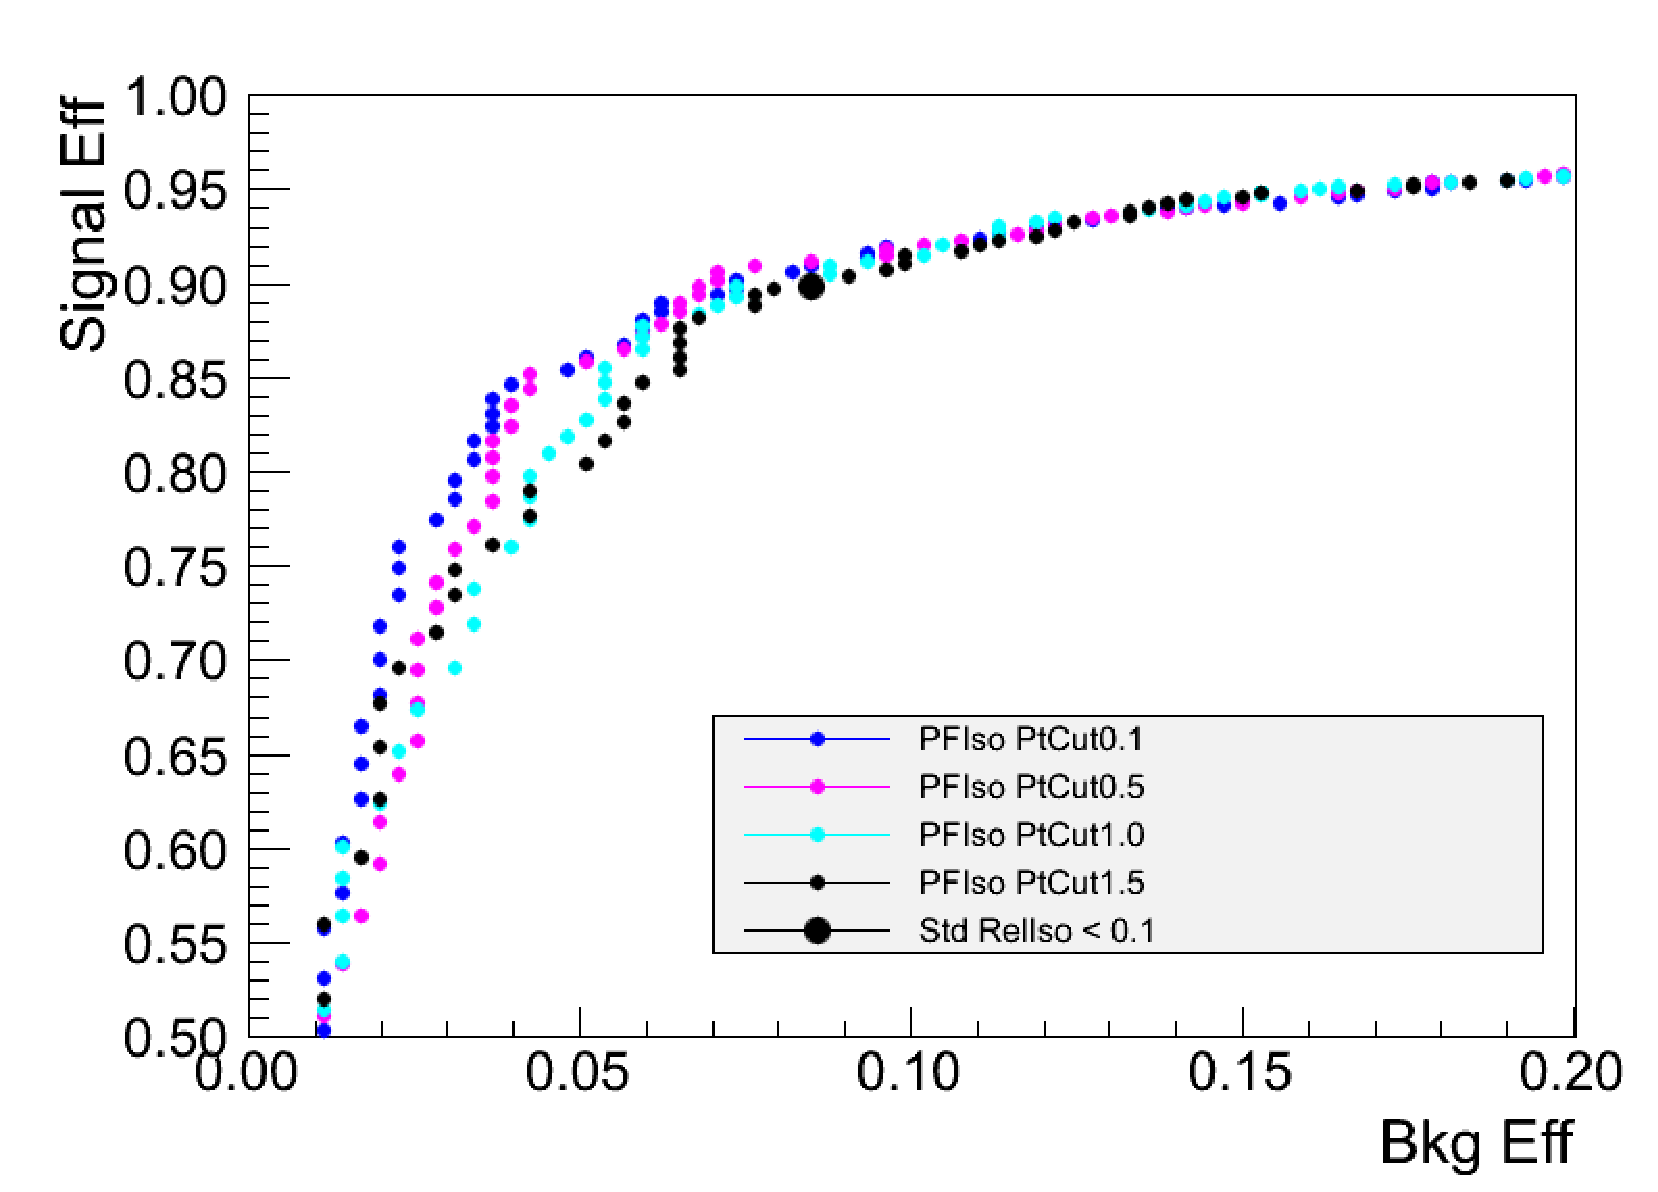
\includegraphics[width=0.48\textwidth]{figures/IsoPerformance_EleBarrel_PtThreshold_NVtx7To15_Pt20To30.pdf}}
\subfigure[Endcap]{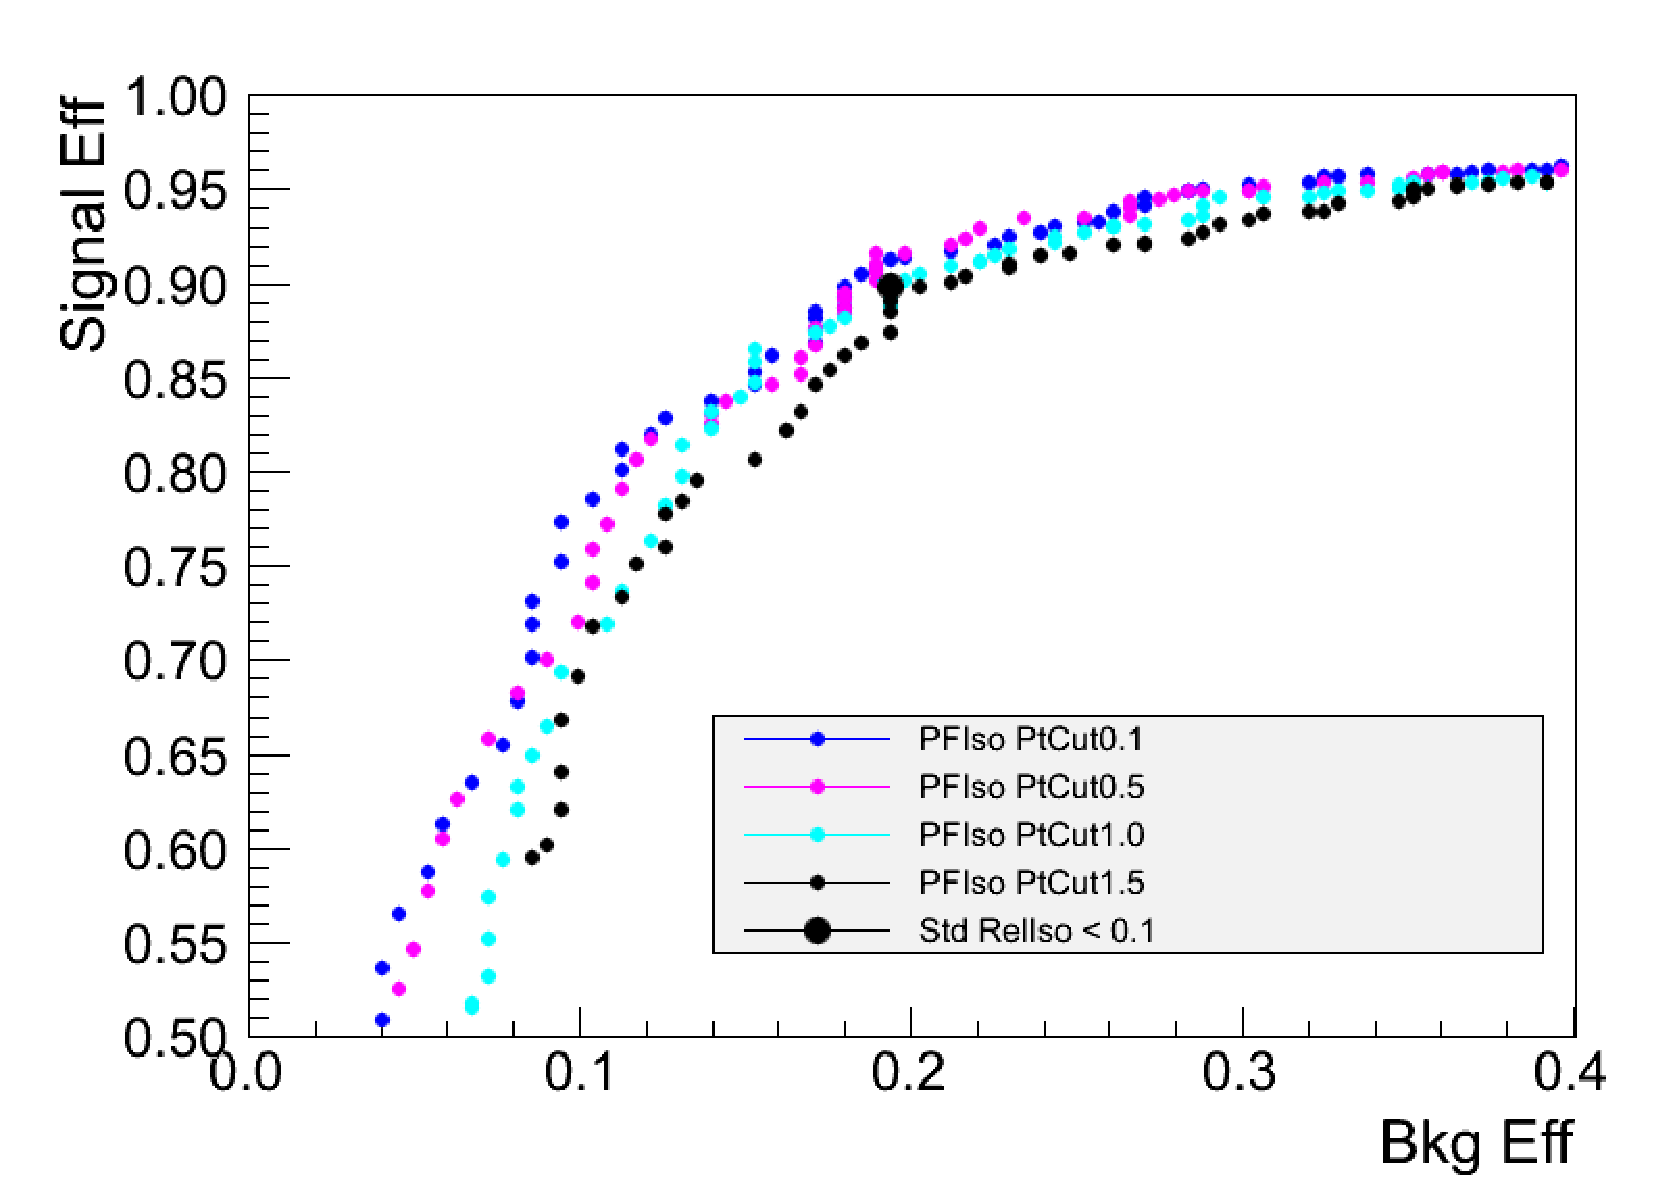
\includegraphics[width=0.48\textwidth]{figures/IsoPerformance_EleEndcap_PtThreshold_NVtx7To15_Pt20To30.pdf}}
\caption{Signal efficiency (HWW130) vs background efficiency for electrons with $p_{T}$ between $20$ and $30$ GeV
separated into barrel and endcap, comparing the effect of applying different $p_{T}$ thresholds on neutral particles.
The high pileup scenario (NVtx $7$-$15$) is shown.}
\label{fig:IsoPerformance_Ele_PtThresholds}
\end{center}
\end{figure}

From here on, we will only compare two variations of the particle flow isolation corrected
for pileup : effective area corrected PF isolation, and PF isolation computed from particles
where a $1$GeV threshold is imposed on the $p_{T}$ of neutrals. The $|\Delta$z$| < 0.1$cm 
cut is applied to all charged particles. In Figure \ref{fig:IsoPerformance_EleBarrel_BestChoices_LowPU}
 we compare the performance of the standard detector based isolation corrected with the effective 
area subtraction scheme with the two variations of PF isolation described above at the pileup 
scenario faced in the first $200$ \ipb of the 2011 data for electrons in the barrel. The working 
point for the standard detector based isolation cut from the WW  cross section measurement with 
$36$ \ipb is marked, along with three additional working points using the particle flow isolation 
with the $0.4$ cone size. We observe that for electrons with $p_{T} < 20$ GeV, there is a 
significant gain in performance for the particle flow isolation. One can gain an additional 
background rejection of $40\%$ with the same signal efficiency at low $p_{T}$. At higher $p_{T}$ 
we observe that the $1$GeV threshold on neutrals begin to hurt the performance, as well as the 
bigger size of the isolation cone. As a result, the particle flow isolation option without
a threshold on neutrals and with the smaller $0.3$ cone is the best performing choice.


\begin{figure}[!htbp]
\begin{center}
\subfigure[$p_{T}$ in $(10,15)$ GeV]{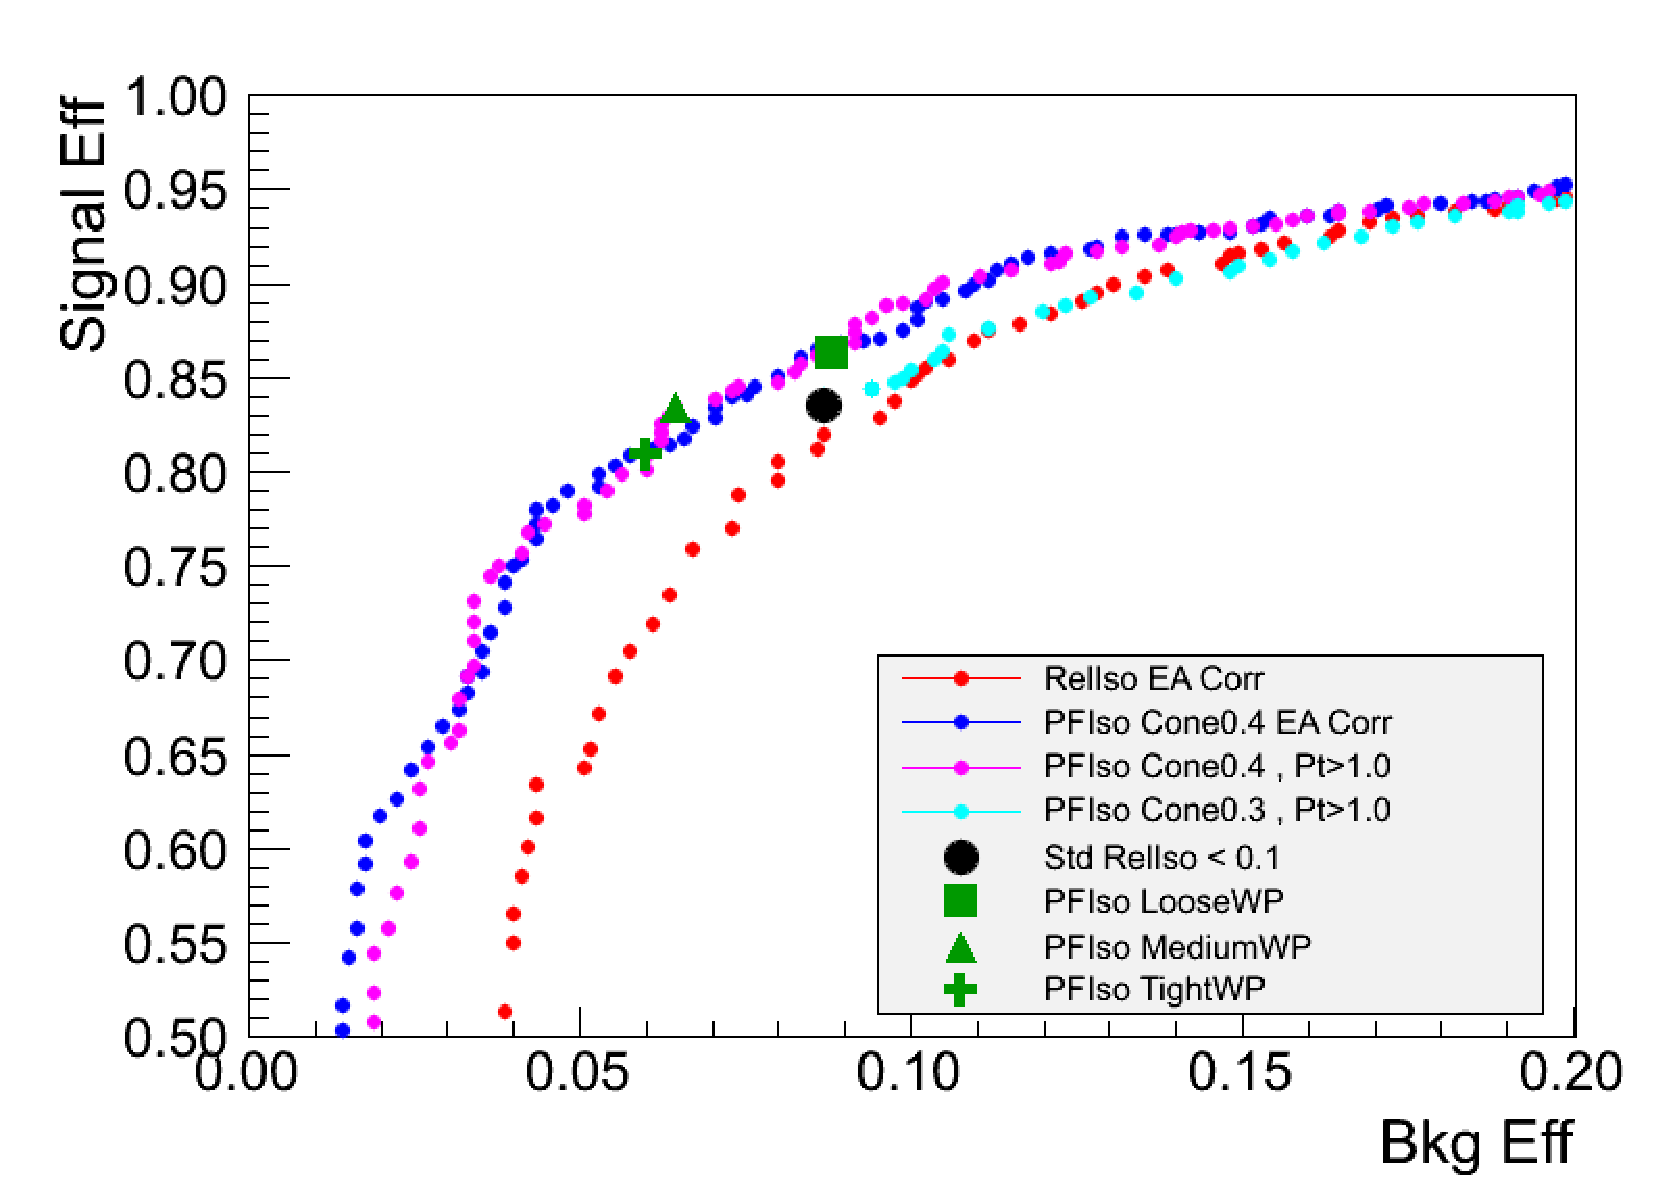
\includegraphics[width=0.48\textwidth]{figures/IsoPerformance_EleBarrel_BestChoices_NVtx3To6_Pt10To15.pdf}}
\subfigure[$p_{T}$ in $(15,20)$ GeV]{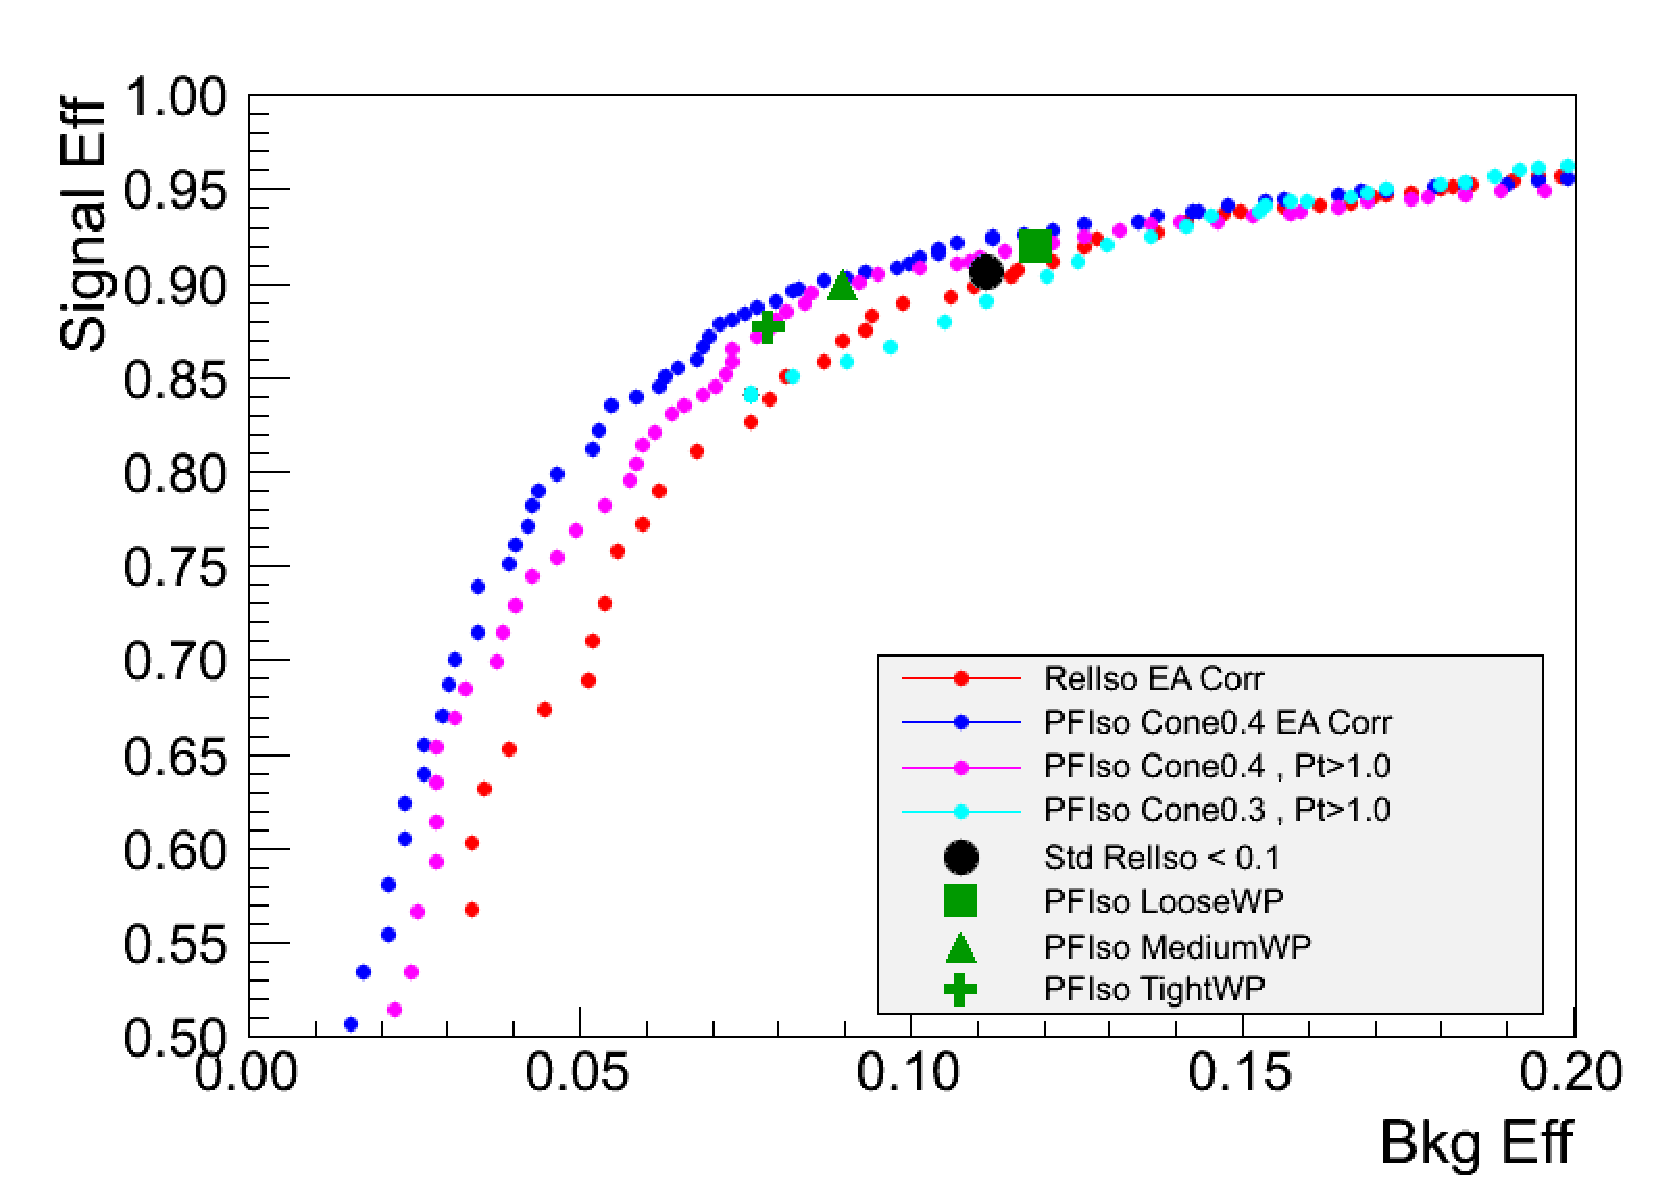
\includegraphics[width=0.48\textwidth]{figures/IsoPerformance_EleBarrel_BestChoices_NVtx3To6_Pt15To20.pdf}}
\subfigure[$p_{T}$ in $(20,30)$ GeV]{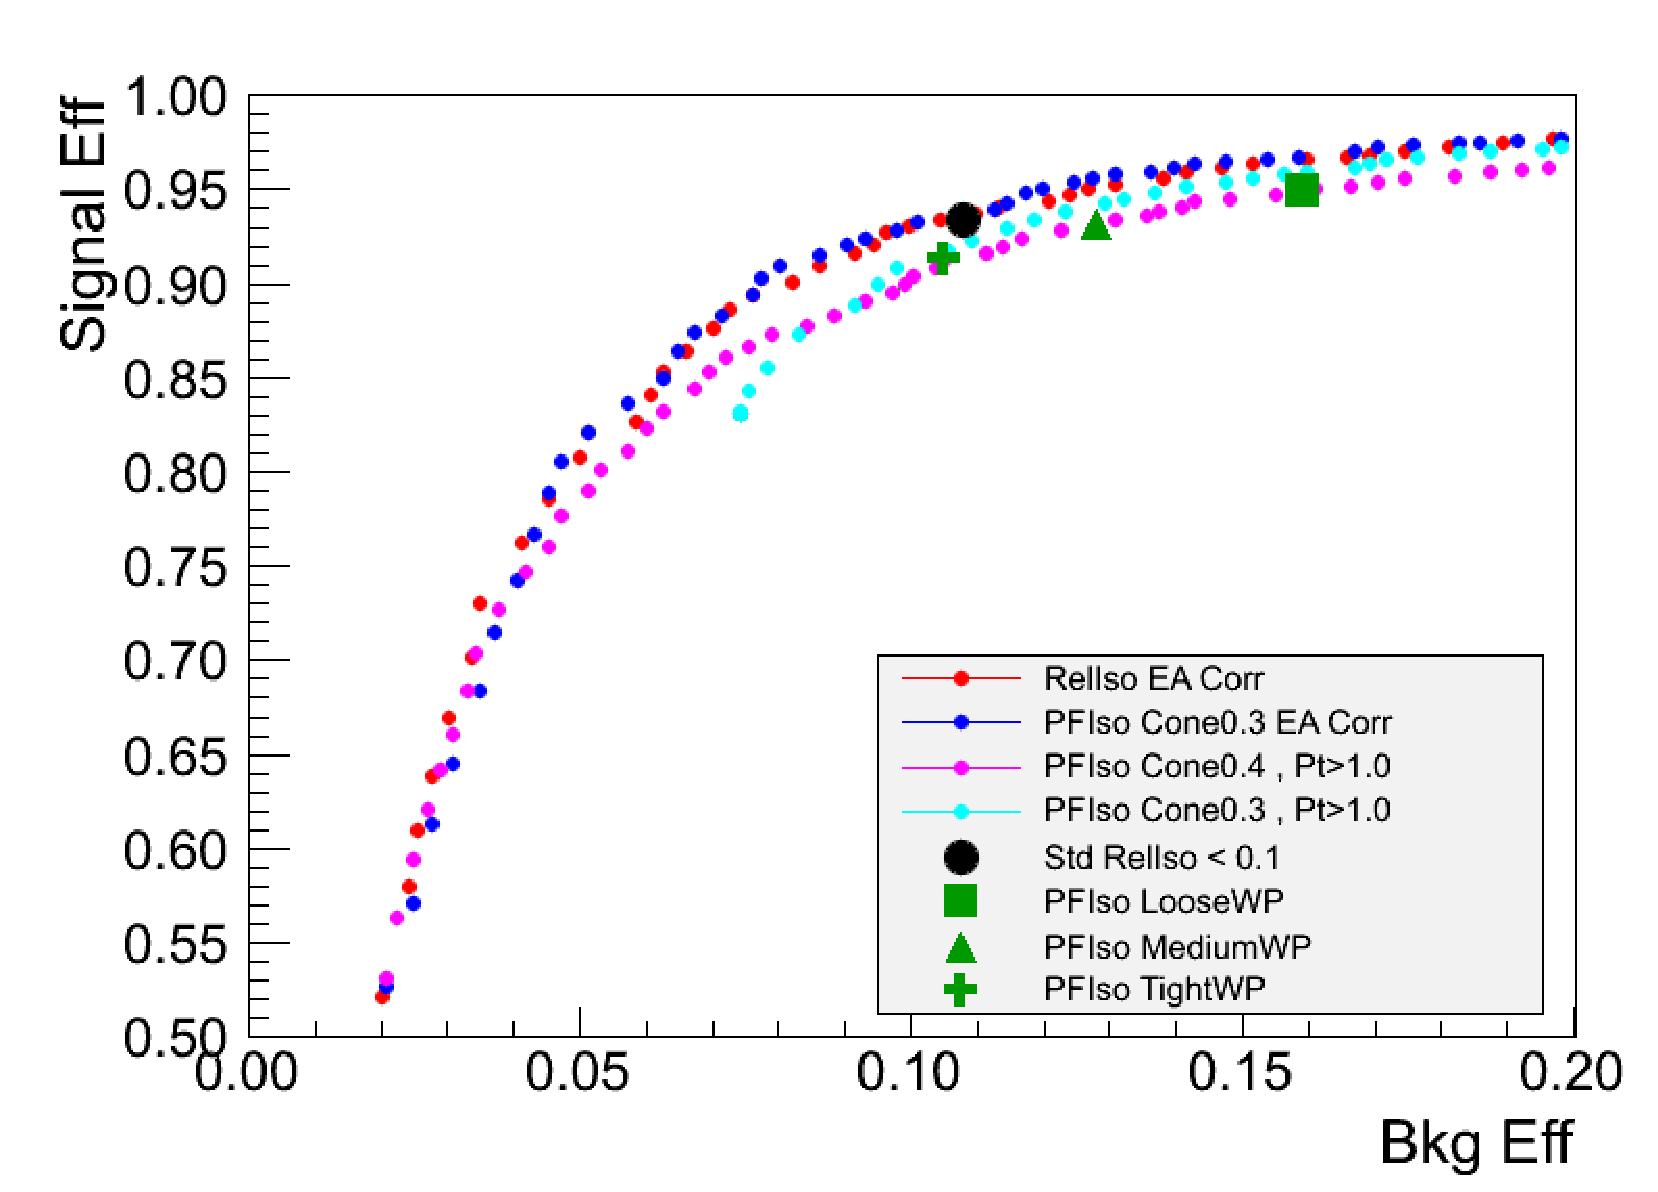
\includegraphics[width=0.48\textwidth]{figures/IsoPerformance_EleBarrel_BestChoicesCone03_NVtx3To6_Pt20To30.pdf}}
\caption{ Signal efficiency (HWW130) vs background efficiency for barrel electrons at low pileup, 
separated into different $p_{T}$ bins, comparing the standard isolation with the best choices .
we have for the particle flow isolation.}
\label{fig:IsoPerformance_EleBarrel_BestChoices_LowPU}
\end{center}
\end{figure}

\clearpage

In Figure \ref{fig:IsoPerformance_EleEndcap_BestChoices_LowPU}, we make the same comparison for 
electrons in the endcap. In the endcap, we observe the the $1$GeV threshold is degrading the 
performance significantly more than in the barrel. For high $p_{T}$, the smaller cone size, again,
gives the best performance. 


\begin{figure}[!htbp]
\begin{center}
\subfigure[$p_{T}$ in $(10,15)$ GeV]{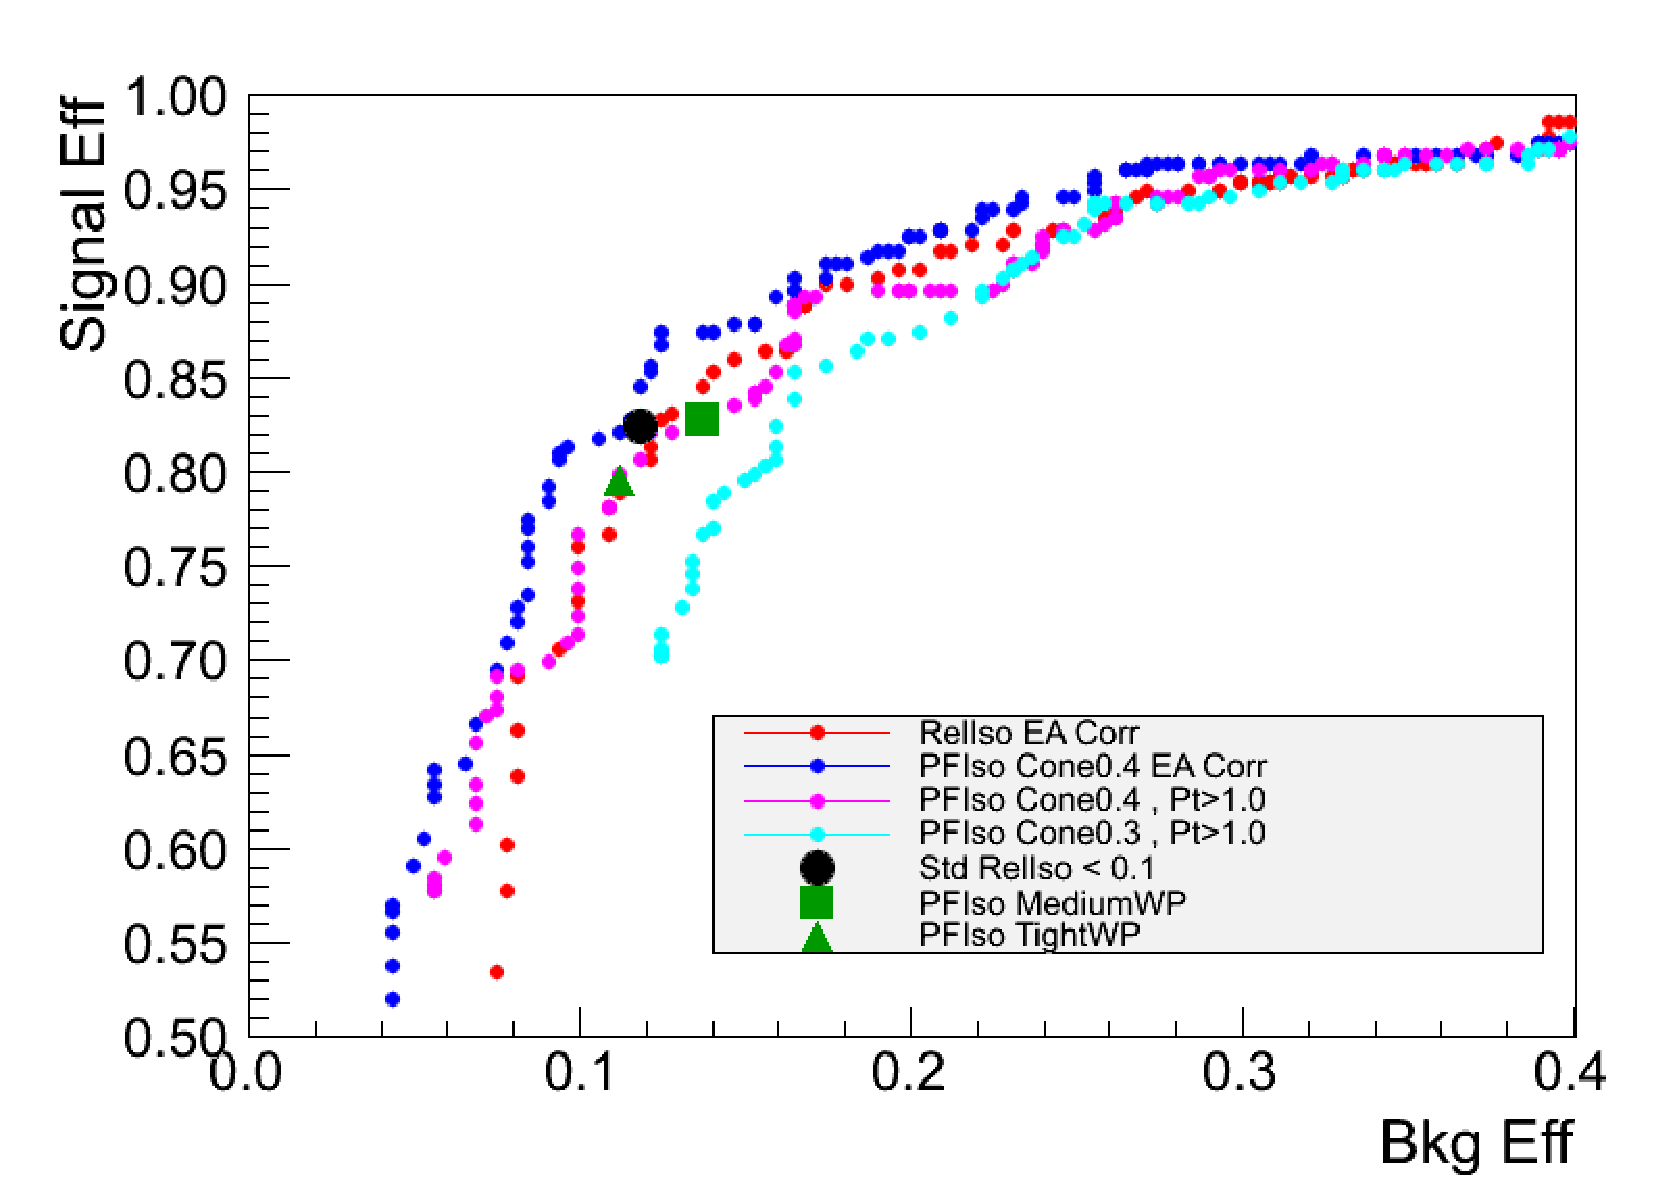
\includegraphics[width=0.48\textwidth]{figures/IsoPerformance_EleEndcap_BestChoices_NVtx3To6_Pt10To15.pdf}}
\subfigure[$p_{T}$ in $(15,20)$ GeV]{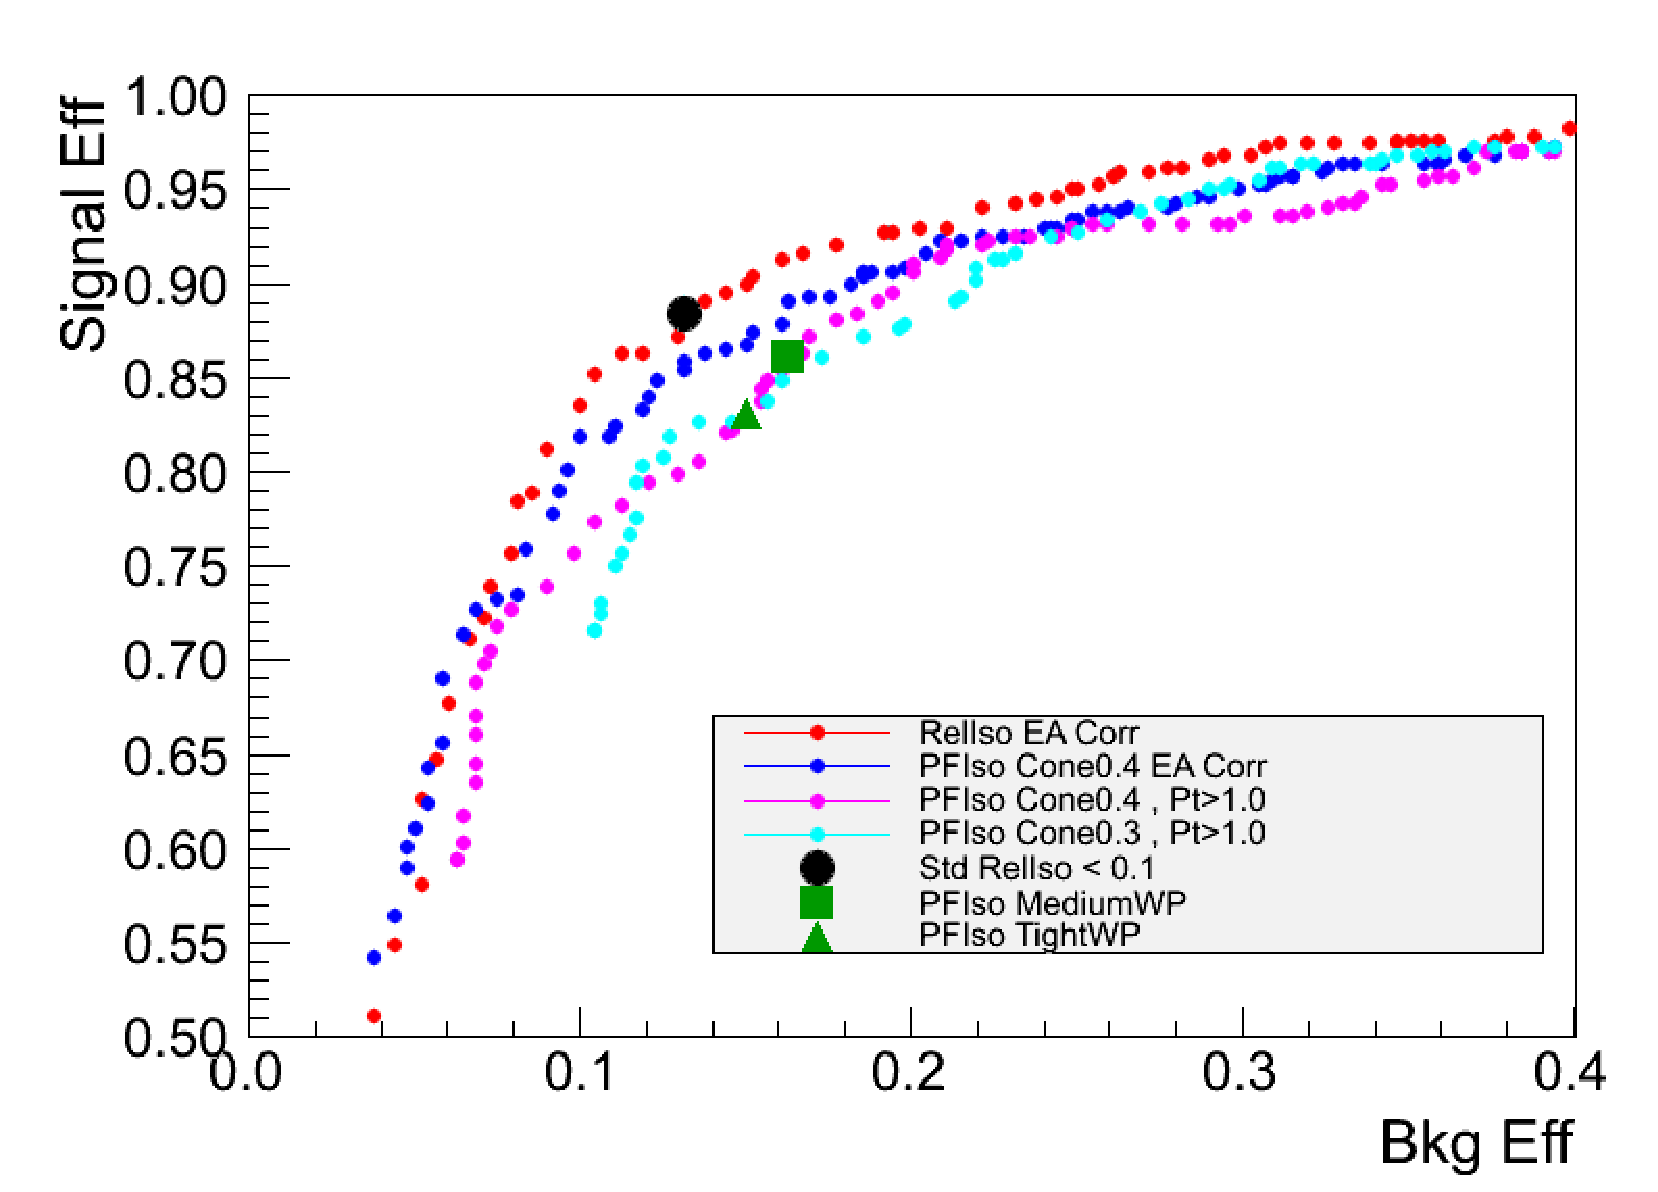
\includegraphics[width=0.48\textwidth]{figures/IsoPerformance_EleEndcap_BestChoices_NVtx3To6_Pt15To20.pdf}}
\subfigure[$p_{T}$ in $(20,30)$ GeV]{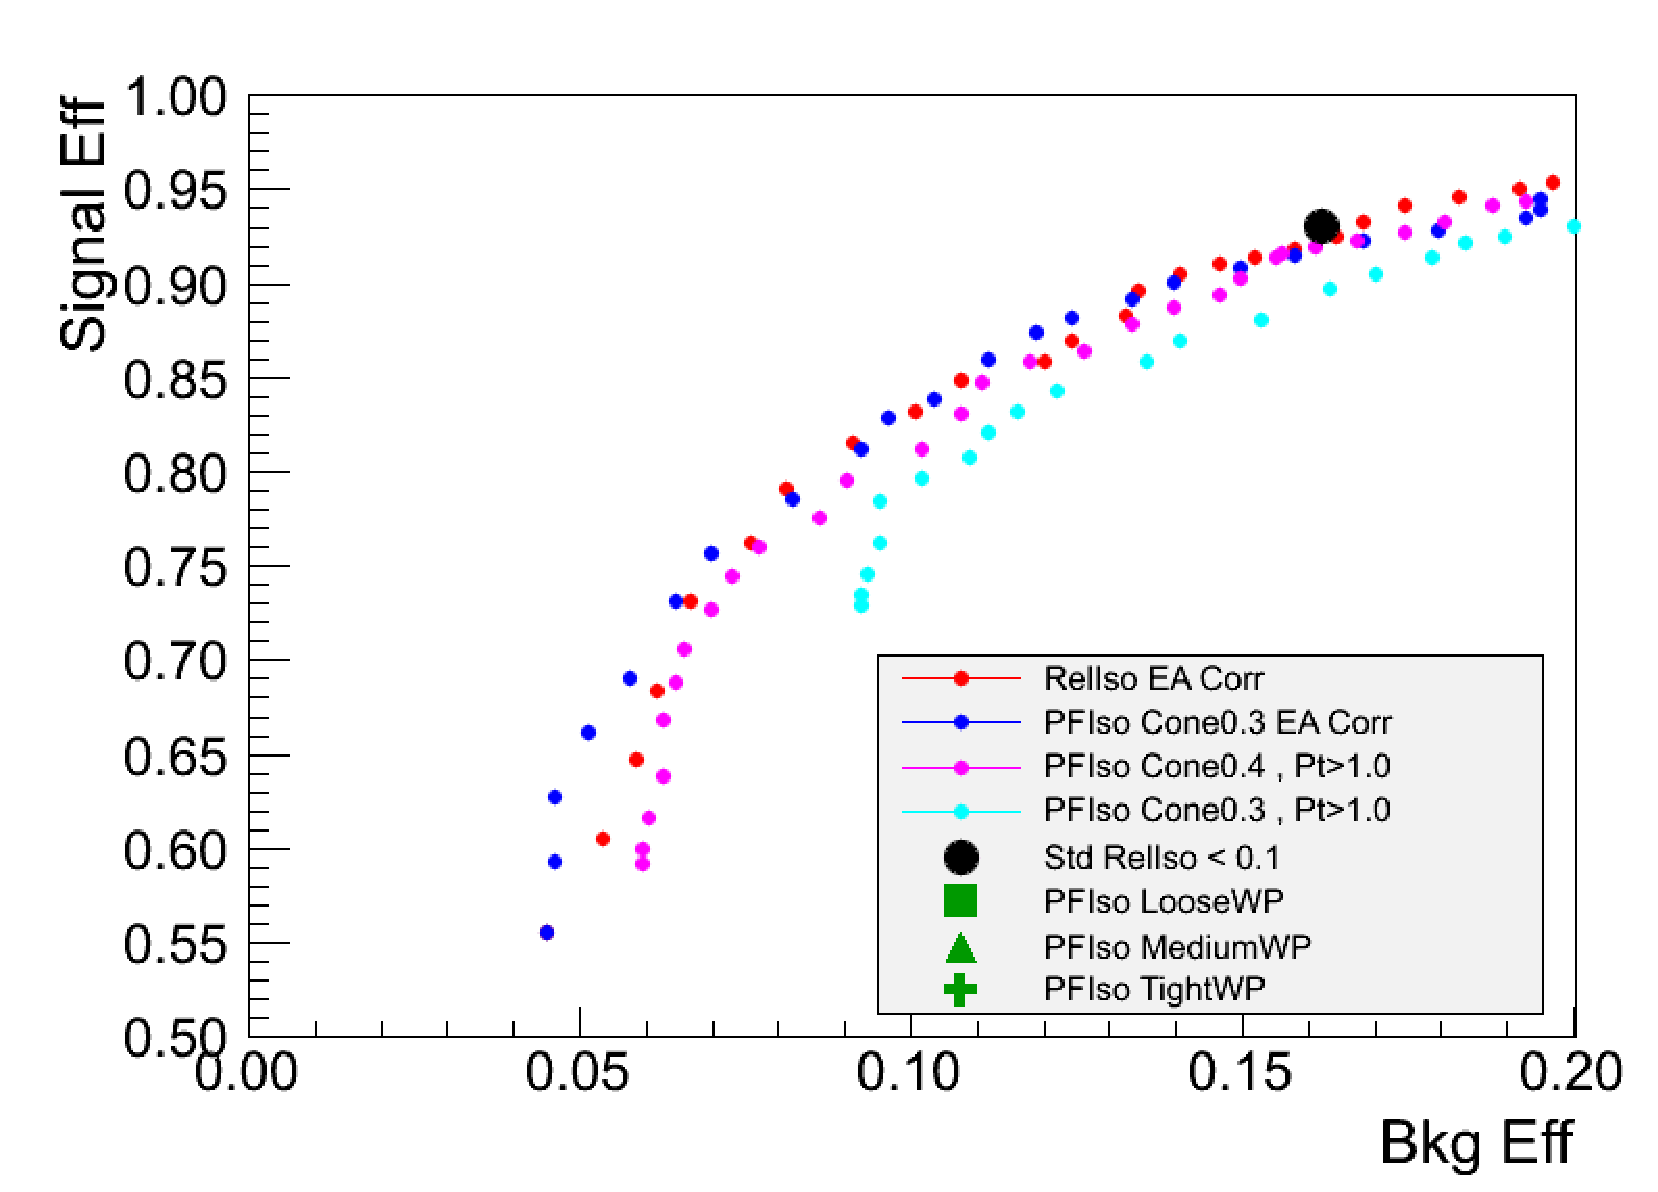
\includegraphics[width=0.48\textwidth]{figures/IsoPerformance_EleEndcap_BestChoicesCone03_NVtx3To6_Pt20To30.pdf}}
\caption{Signal efficiency (HWW130) vs background efficiency for endcap electrons at low pileup
separated into different $p_{T}$ bins, comparing the standard isolation with the best choices .
we have for the particle flow isolation.}
\label{fig:IsoPerformance_EleEndcap_BestChoices_LowPU}
\end{center}
\end{figure}

\clearpage

In Figure \ref{fig:IsoPerformance_EleBarrel_BestChoices_HighPU}, we make the same comparison again for the
barrel but with a much more severe pileup scenario, selecting events with the number of reconstructed
vertices between $7$ and $15$. At high pileup, we observe a huge gain in performance for the particle
flow isolation relative to the detector based isolation. At higher $p_{T}$ we are again being 
adversely affected by the $1$ GeV threshold, and to a lesser degree the larger cone size. The
best performing option is the particle flow isolation with the smaller $0.3$ cone and no threshold
on neutrals.




\begin{figure}[!htbp]
\begin{center}
\subfigure[$p_{T}$ in $(10,15)$ GeV]{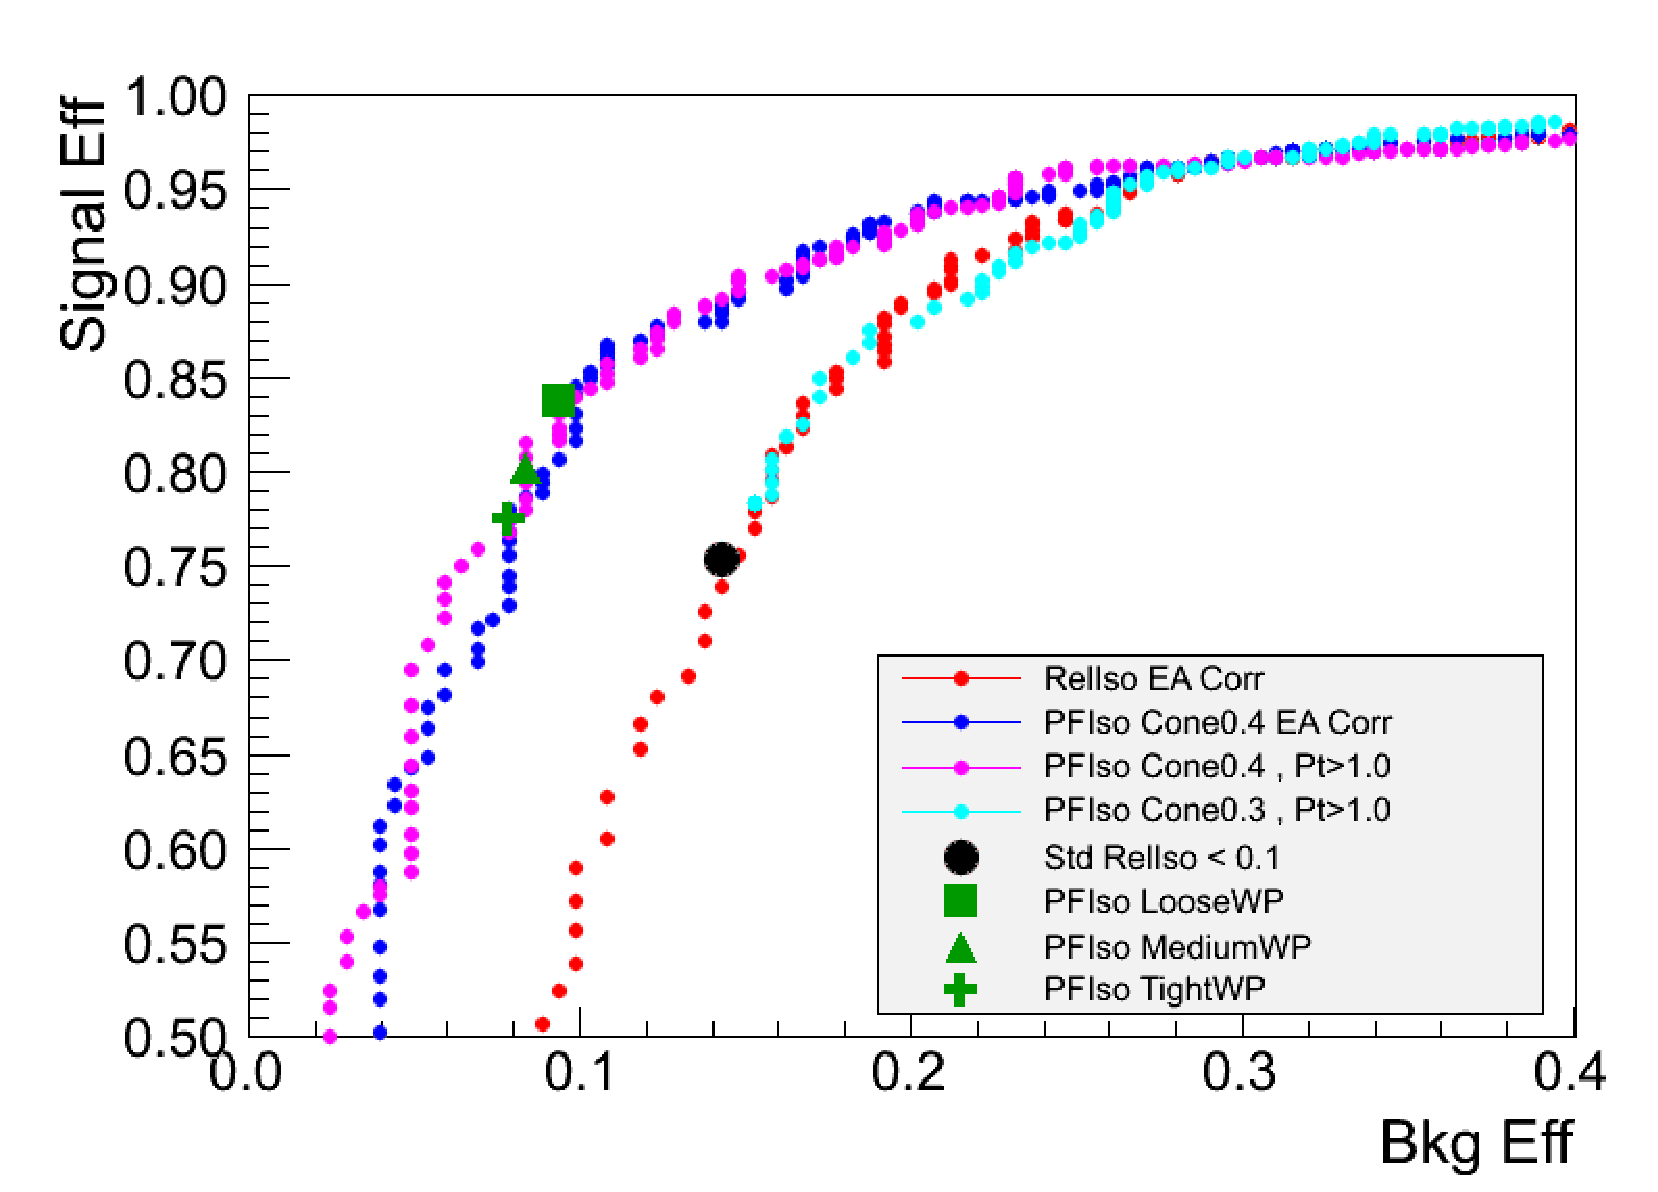
\includegraphics[width=0.48\textwidth]{figures/IsoPerformance_EleBarrel_BestChoices_NVtx7To15_Pt10To15.pdf}}
\subfigure[$p_{T}$ in $(15,20)$ GeV]{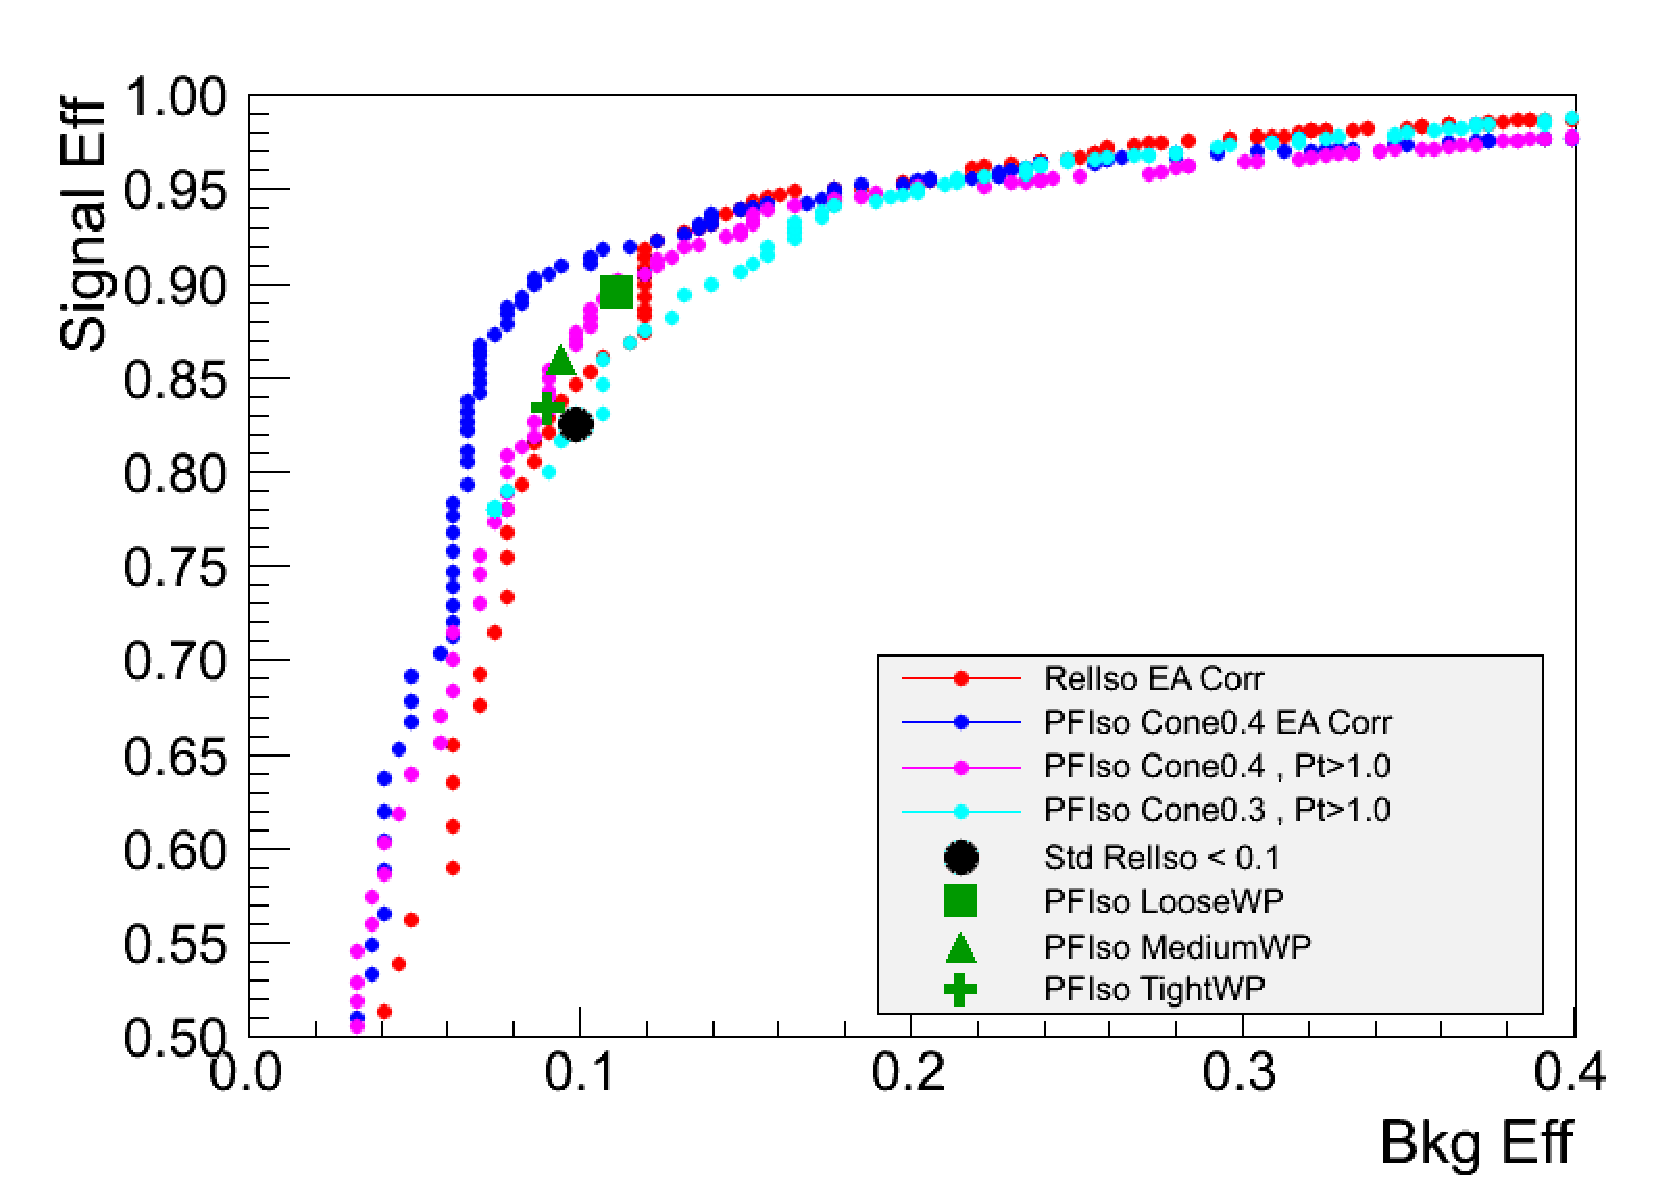
\includegraphics[width=0.48\textwidth]{figures/IsoPerformance_EleBarrel_BestChoices_NVtx7To15_Pt15To20.pdf}}
\subfigure[$p_{T}$ in $(20,30)$ GeV]{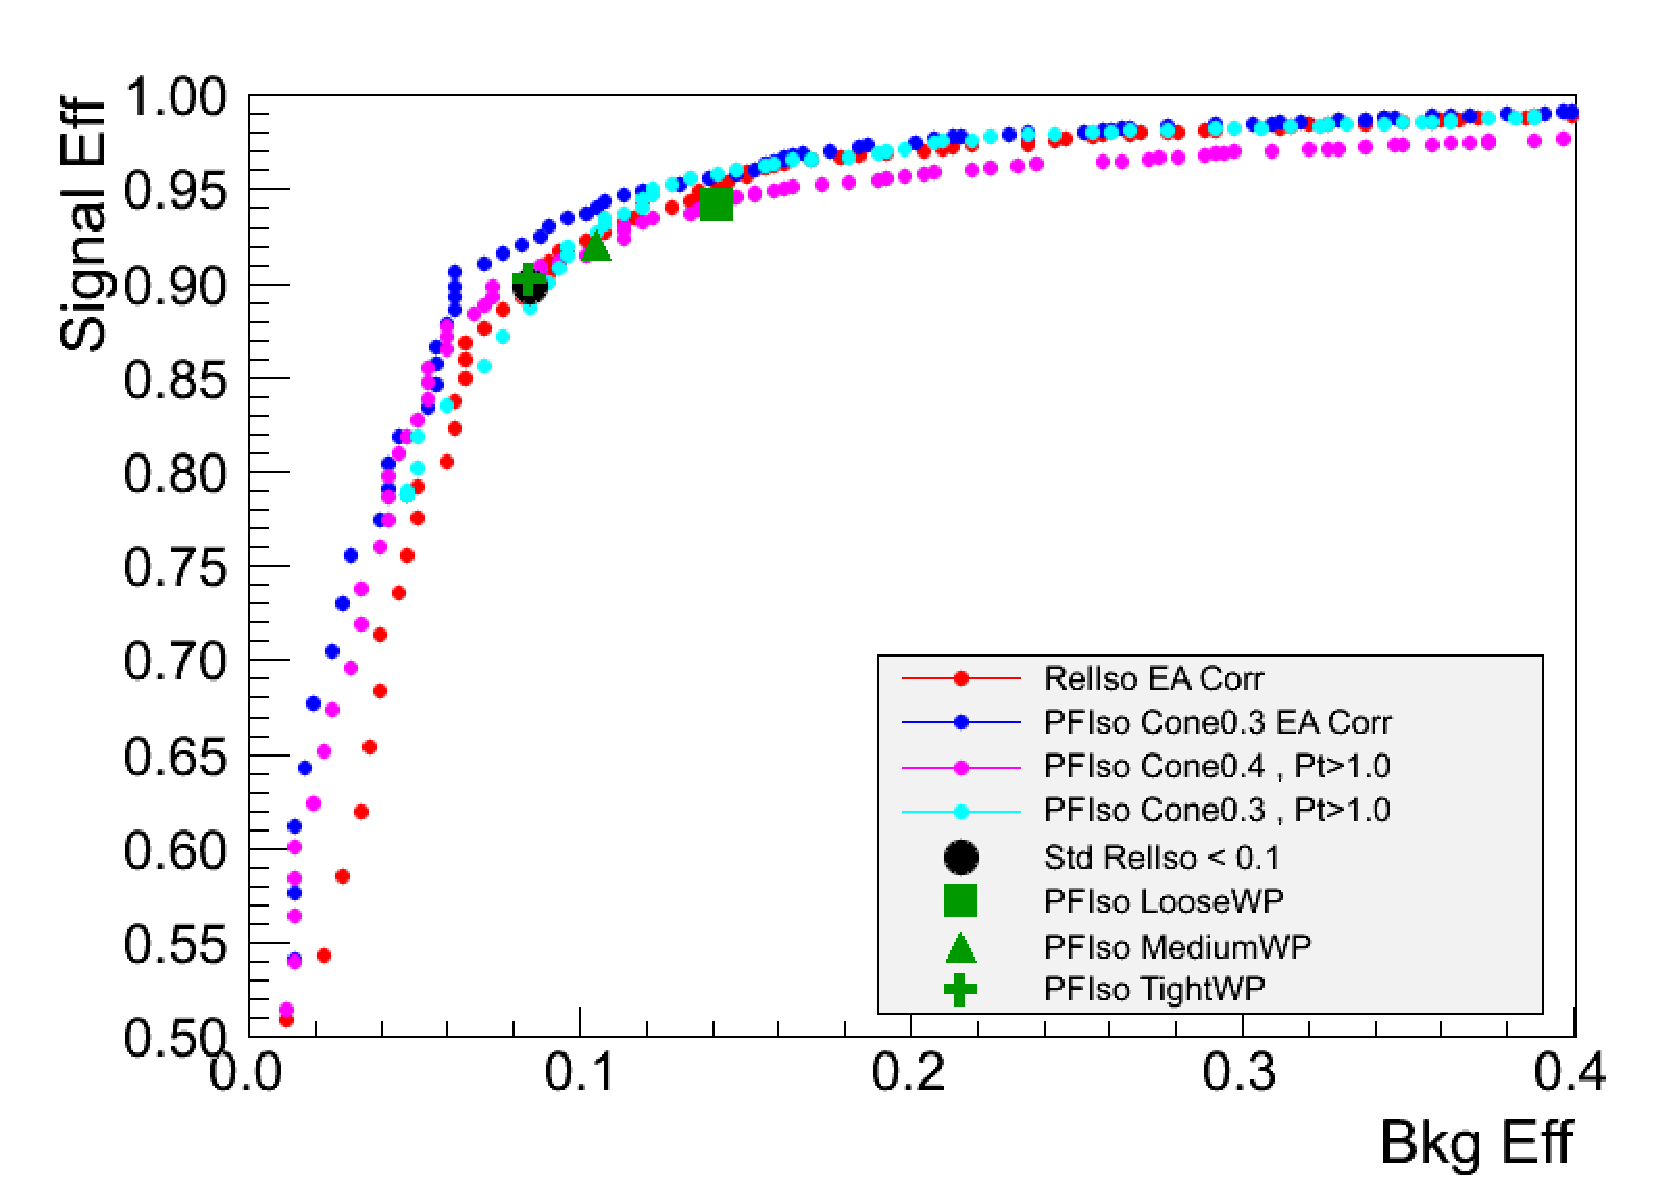
\includegraphics[width=0.48\textwidth]{figures/IsoPerformance_EleBarrel_BestChoicesCone03_NVtx7To15_Pt20To30.pdf}}
\caption{Signal efficiency (HWW130) vs background efficiency for barrel electrons at high pileup
separated into different $p_{T}$ bins, comparing the standard isolation with the best choices .
we have for the particle flow isolation.}
\label{fig:IsoPerformance_EleBarrel_BestChoices_HighPU}
\end{center}
\end{figure}

\clearpage

In Figure \ref{fig:IsoPerformance_EleEndcap_BestChoices_HighPU}, we perform the same comparison for
the endcap at high pileup. Here we suffer from limited statistics in the background estimate
due to the fact that in the first $200$ \ipb of data in 2011, we did not have many events with
such high pileup conditions. Similar general trends can still be observed, however. At higher
$p_{T}$ we observe some degradation due to the $1GeV$ threshold on neutrals, and also the larger
cone size. In this case, the detector based isolation is performing the best.

\begin{figure}[!htbp]
\begin{center}
\subfigure[$p_{T}$ in $(10,15)$ GeV]{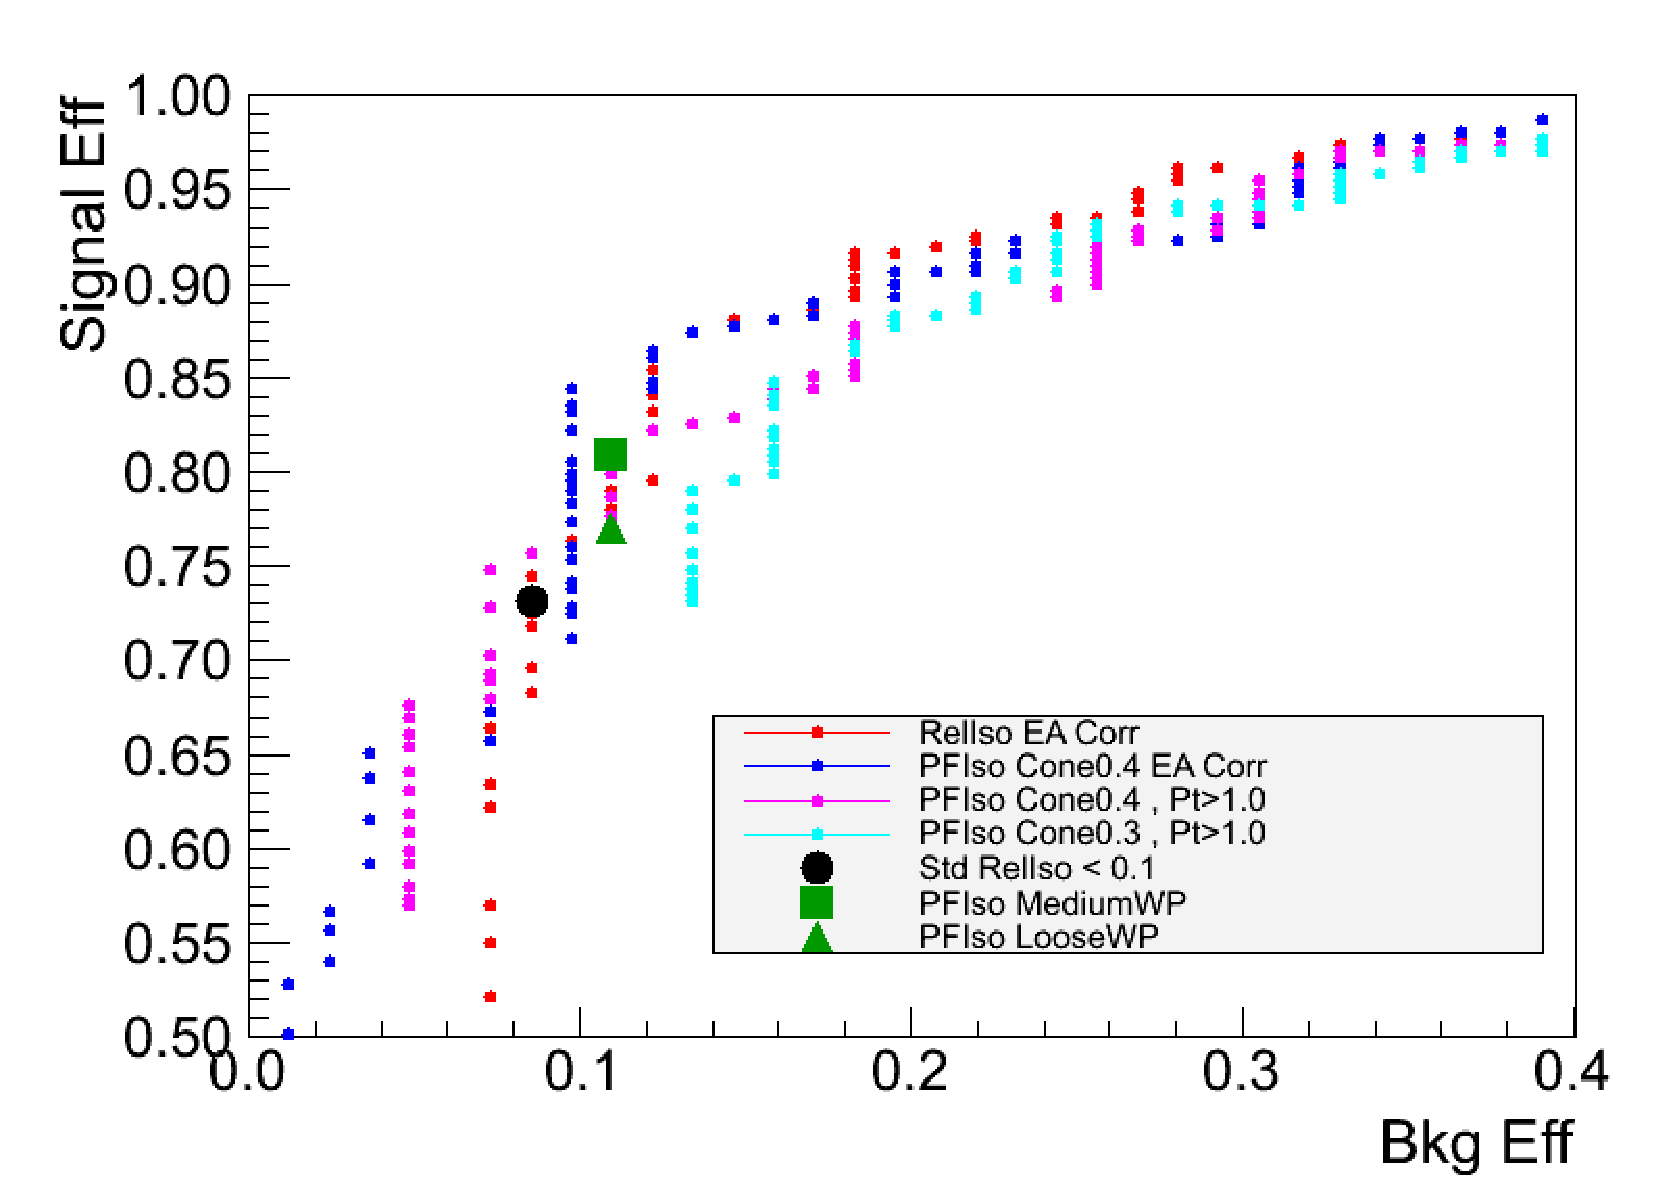
\includegraphics[width=0.48\textwidth]{figures/IsoPerformance_EleEndcap_BestChoices_NVtx7To15_Pt10To15.pdf}}
\subfigure[$p_{T}$ in $(15,20)$ GeV]{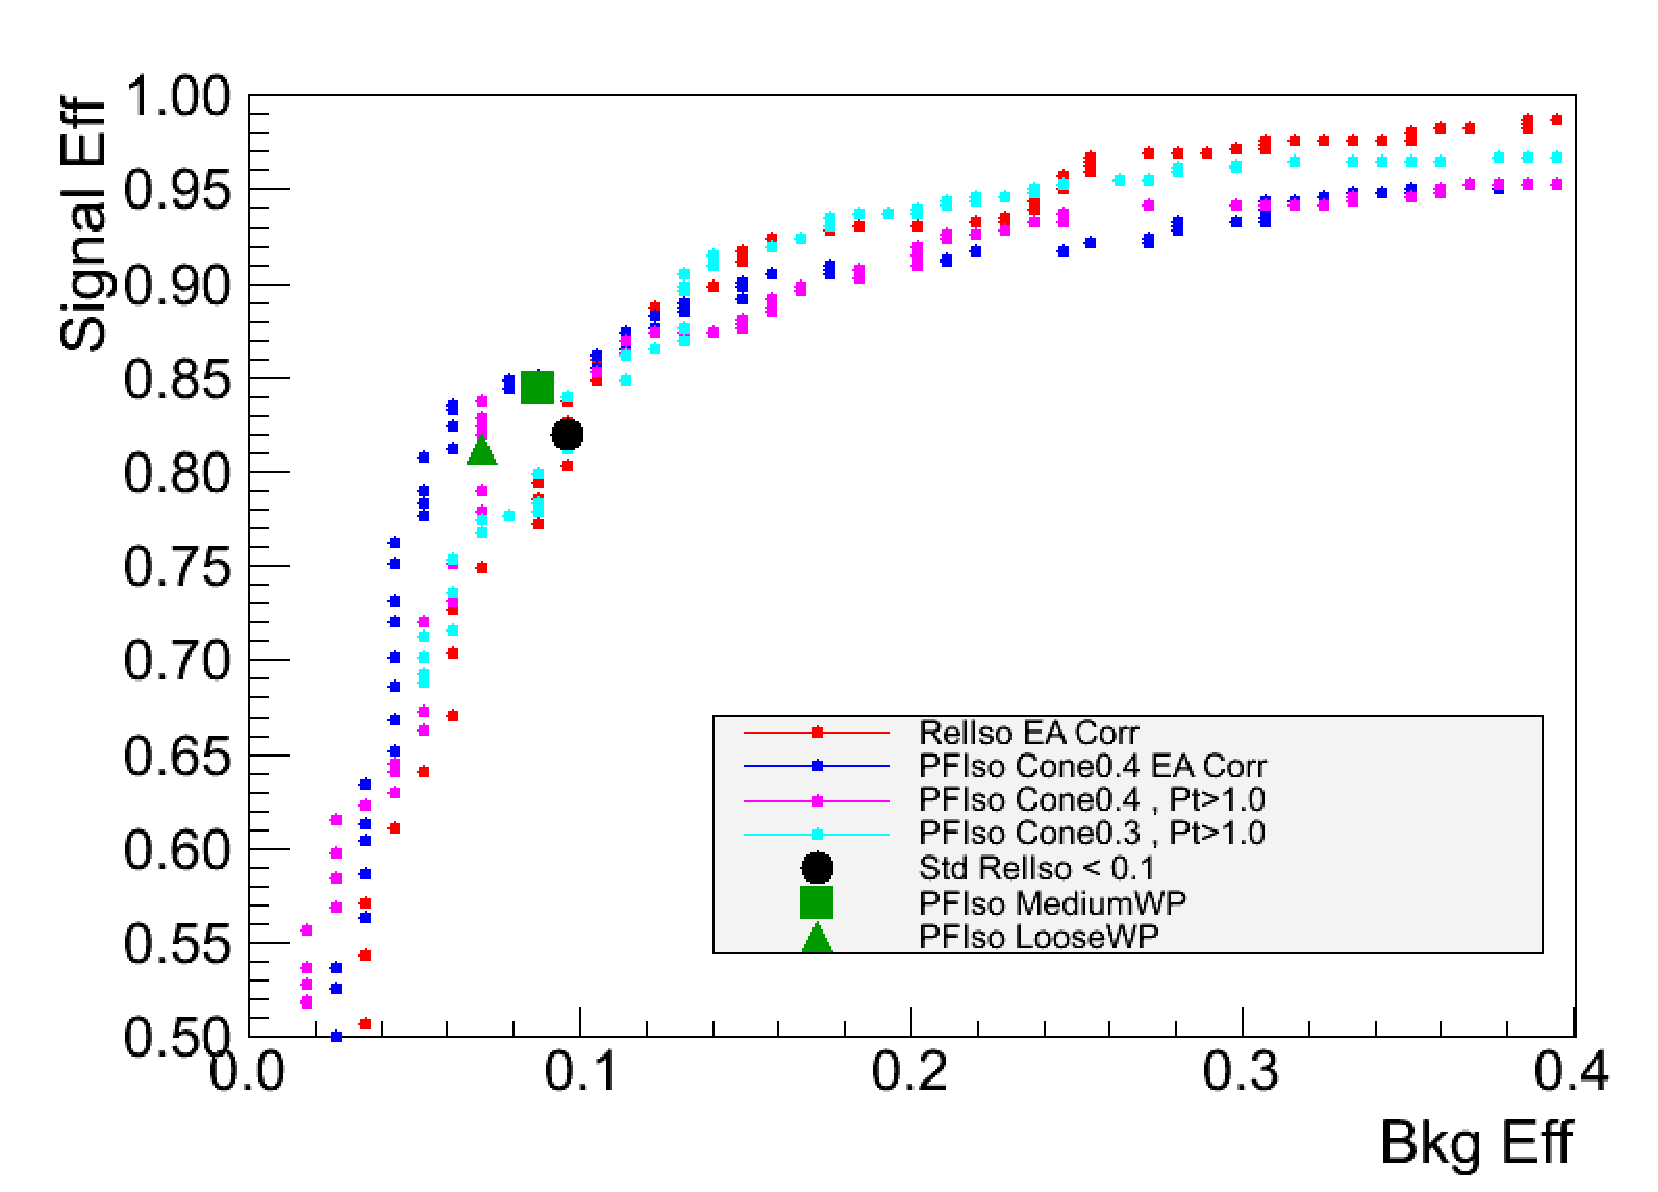
\includegraphics[width=0.48\textwidth]{figures/IsoPerformance_EleEndcap_BestChoices_NVtx7To15_Pt15To20.pdf}}
\subfigure[$p_{T}$ in $(20,30)$ GeV]{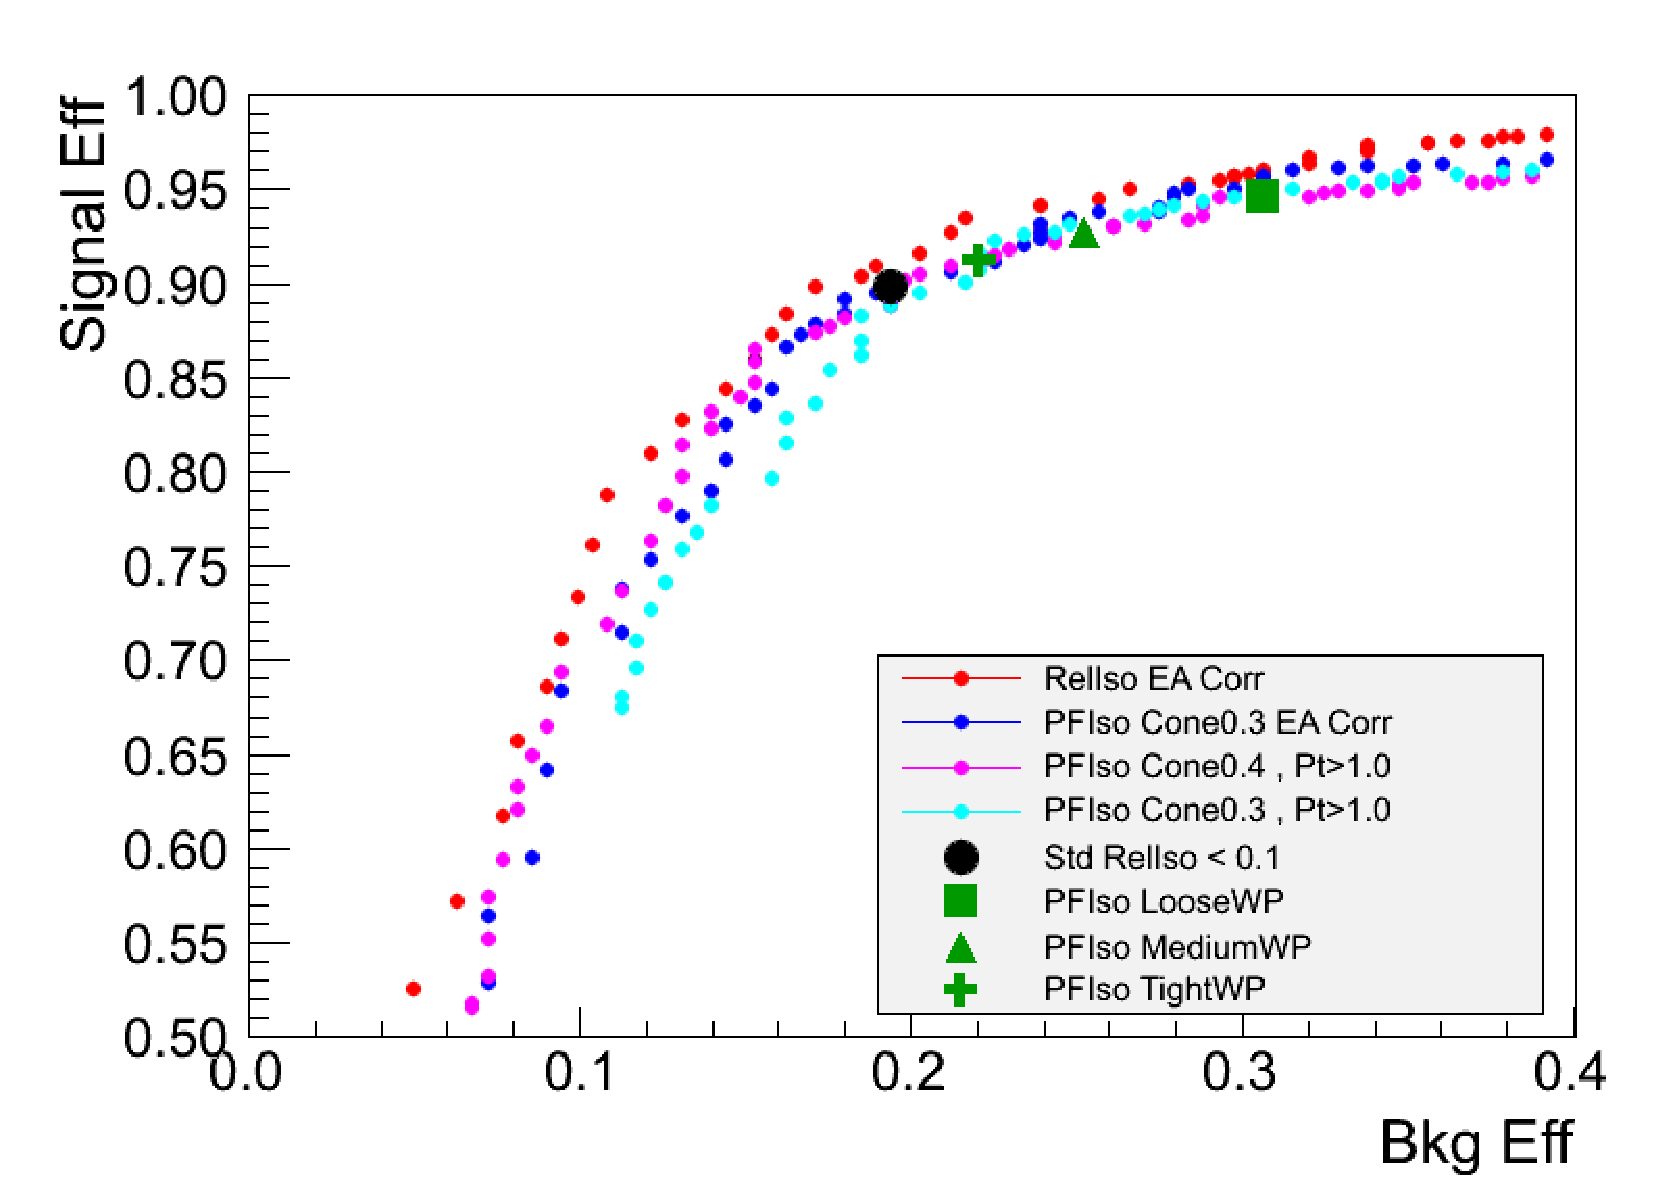
\includegraphics[width=0.48\textwidth]{figures/IsoPerformance_EleEndcap_BestChoicesCone03_NVtx7To15_Pt20To30.pdf}}
\caption{Signal efficiency (HWW130) vs background efficiency for endcap electrons at high pileup
separated into different $p_{T}$ bins, comparing the standard isolation with the best choices .
we have for the particle flow isolation.}
\label{fig:IsoPerformance_EleEndcap_BestChoices_HighPU}
\end{center}
\end{figure}

\clearpage




For the particle flow isolation with the $1$GeV threshold on neutrals and a cone size of $0.4$, we study the isolation
efficiency as a function of the number of reconstructed vertices in the Higgs Monte Carlo simulation with a higgs 
mass of $130$ GeV. Figures \ref{fig:EleIsoEffVsNVtx_PFIso_Pt10To15} and \ref{fig:EleIsoEffVsNVtx_PFIso_Pt20To30}
show the decrease in efficiency with more pileup for low and high $p_{T}$ electrons respectively. In Table 
\ref{tab:EleIsoEfficiency_LossFromPileup_CompareStdWithPF}, we compare the efficiency loss from no pileup 
to $10$ reconstructed primary vertices for the standard detector based isolation cut and the particle flow
isolation cut with the $1$ GeV threshold on neutral particles. We see that there is a significant decrease
in the sensitivity of the isolation efficiency to the presence of pileup when we move to the particle 
flow isolation cut.


\begin{figure}[!htbp]
\begin{center}
\subfigure[Barrel]{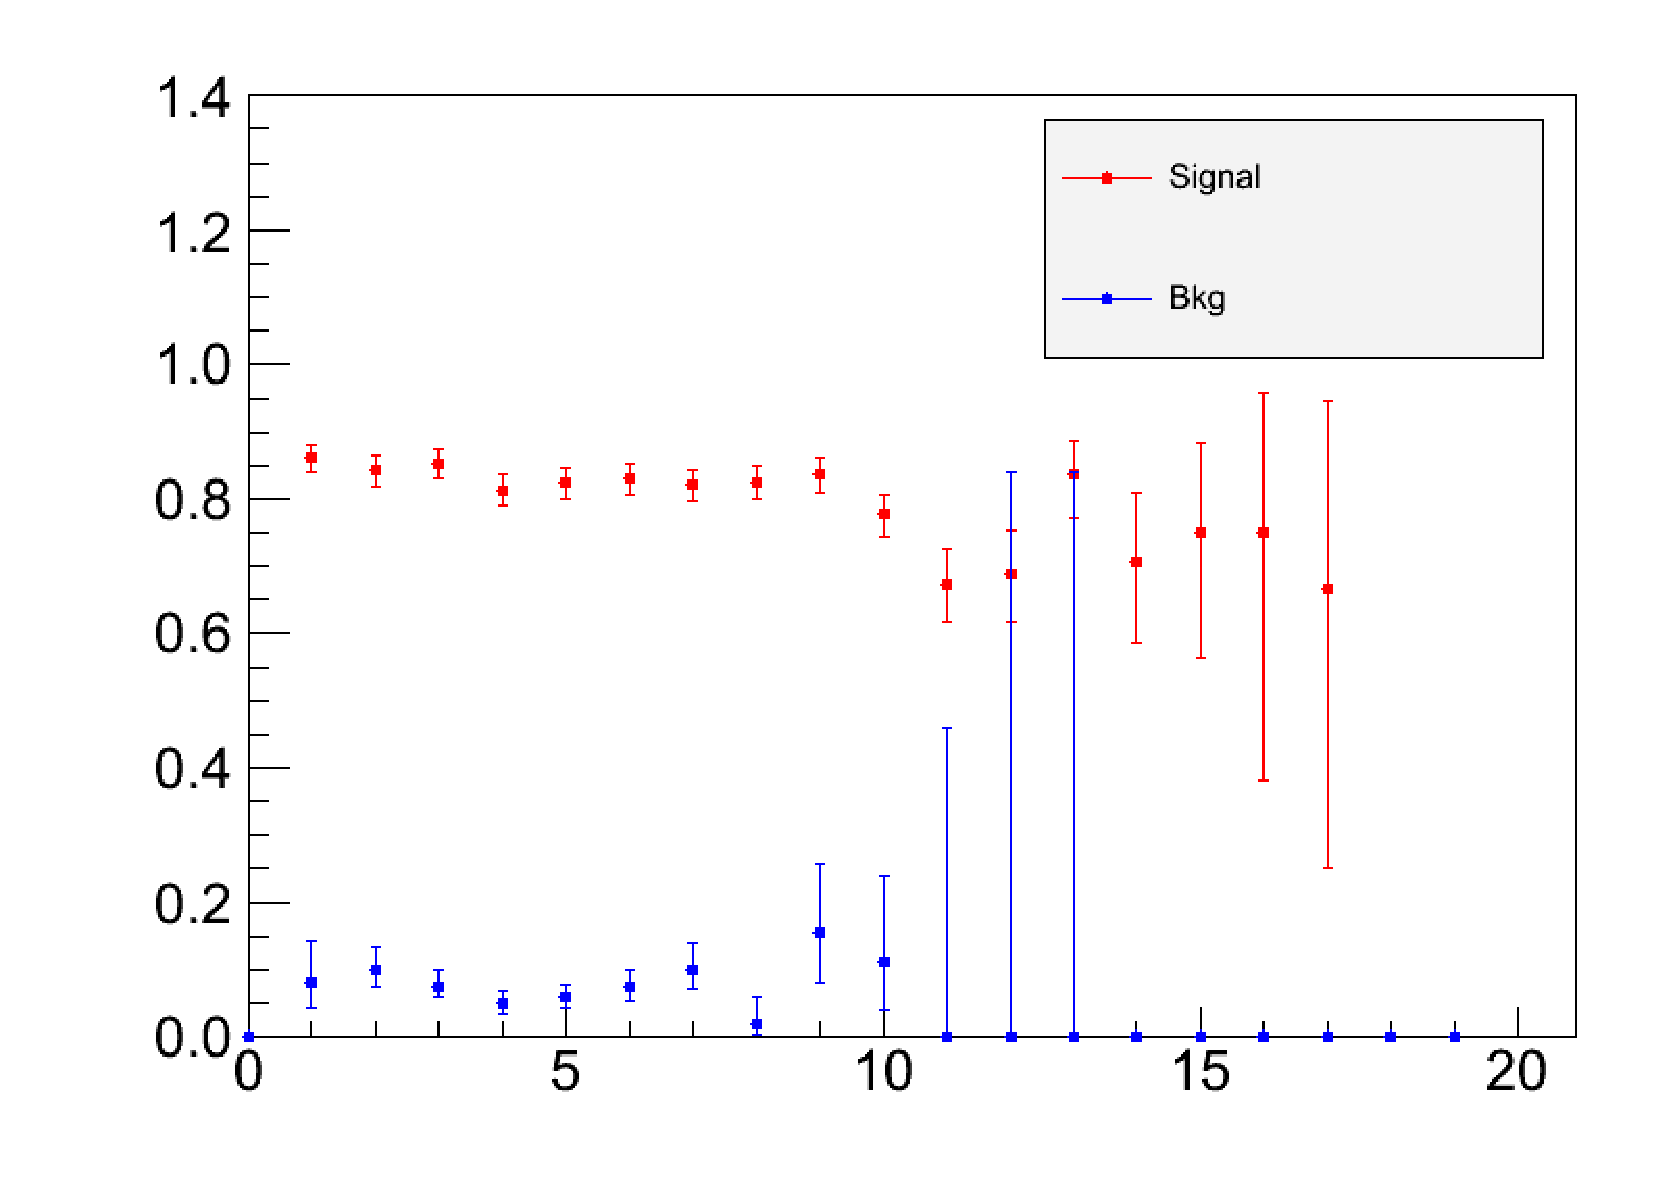
\includegraphics[width=0.48\textwidth]{figures/EleIsoEffVsNVtx_PFIso_Barrel_Pt10To15.pdf}}
\subfigure[Endcap]{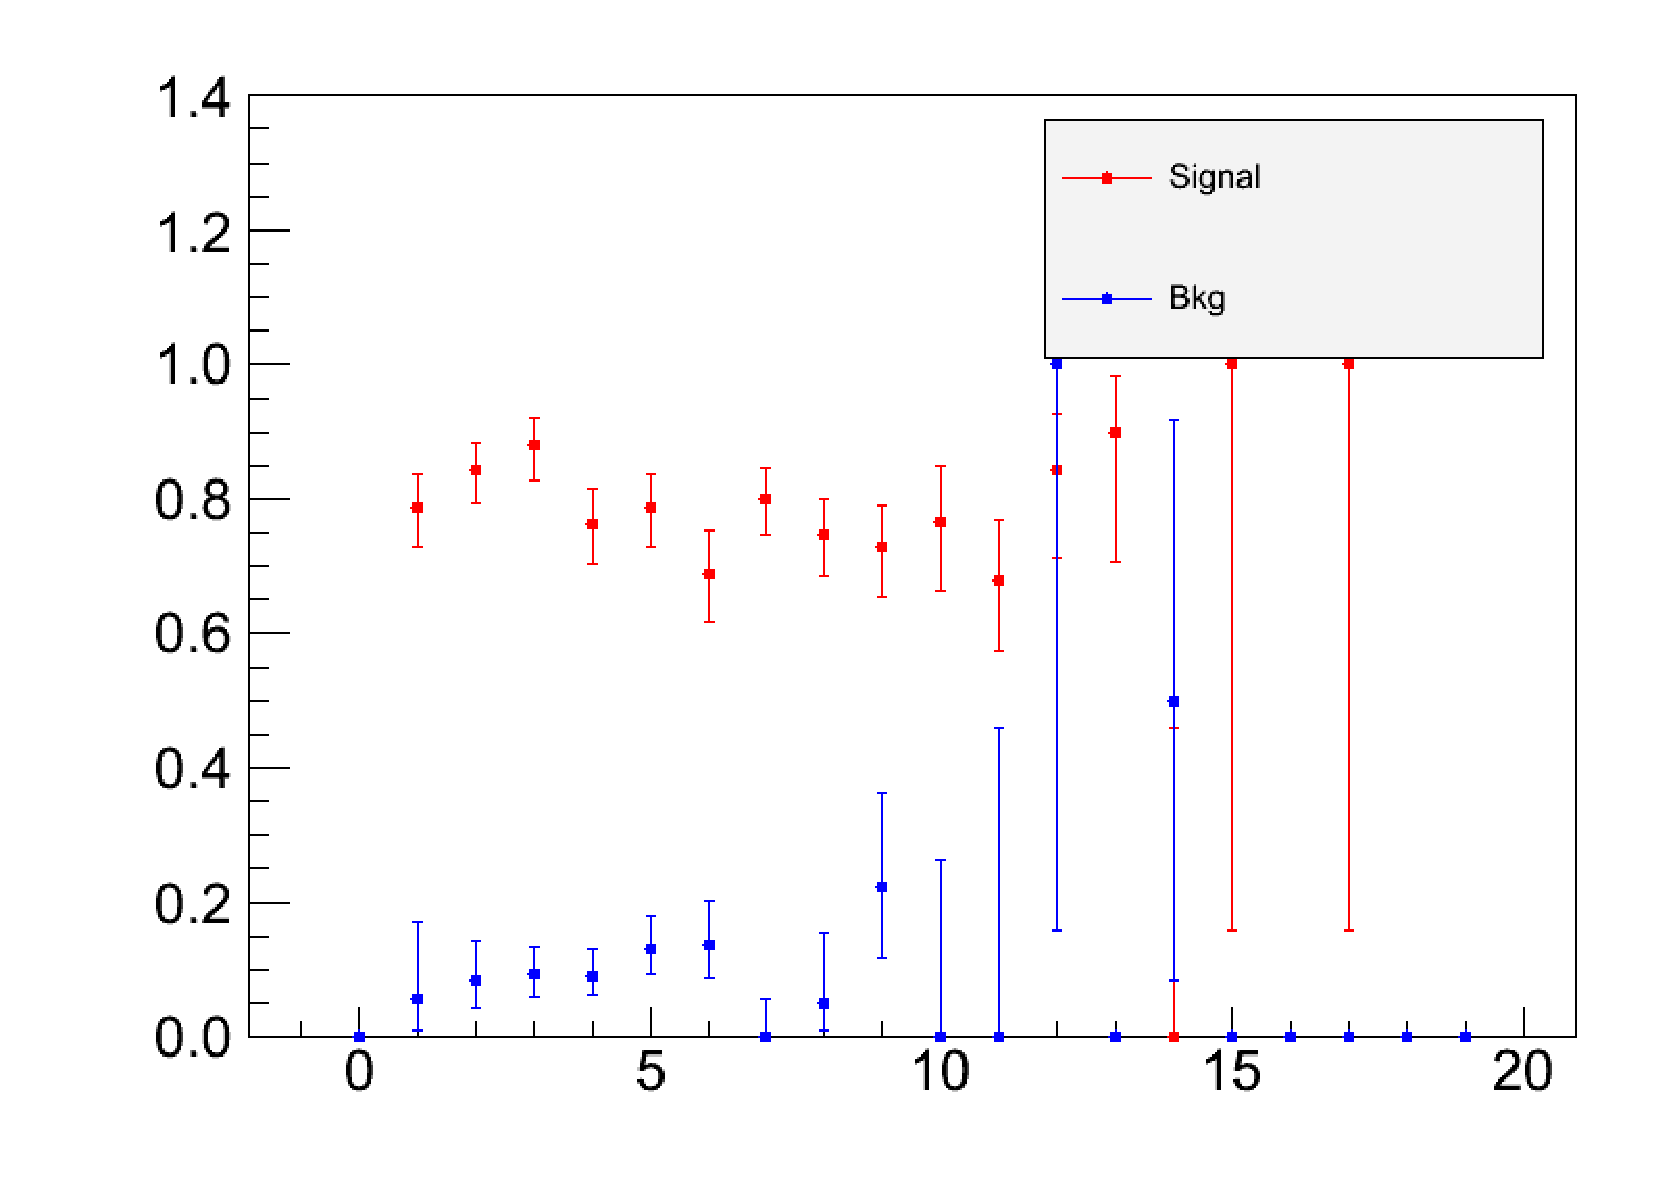
\includegraphics[width=0.48\textwidth]{figures/EleIsoEffVsNVtx_PFIso_Endcap_Pt10To15.pdf}}
\caption{The isolation efficiency of the particle flow isolation cut with the $1$GeV threshold on neutrals
for leptons with $p_{T}$ between $10$ and $15$ GeV in the HWW130 signal sample as a function of the 
number of reconstructed primary vertices, for barrel and endcap electrons.  }
\label{fig:EleIsoEffVsNVtx_PFIso_Pt10To15}
\end{center}
\end{figure}

\begin{figure}[!htbp]
\begin{center}
\subfigure[Barrel]{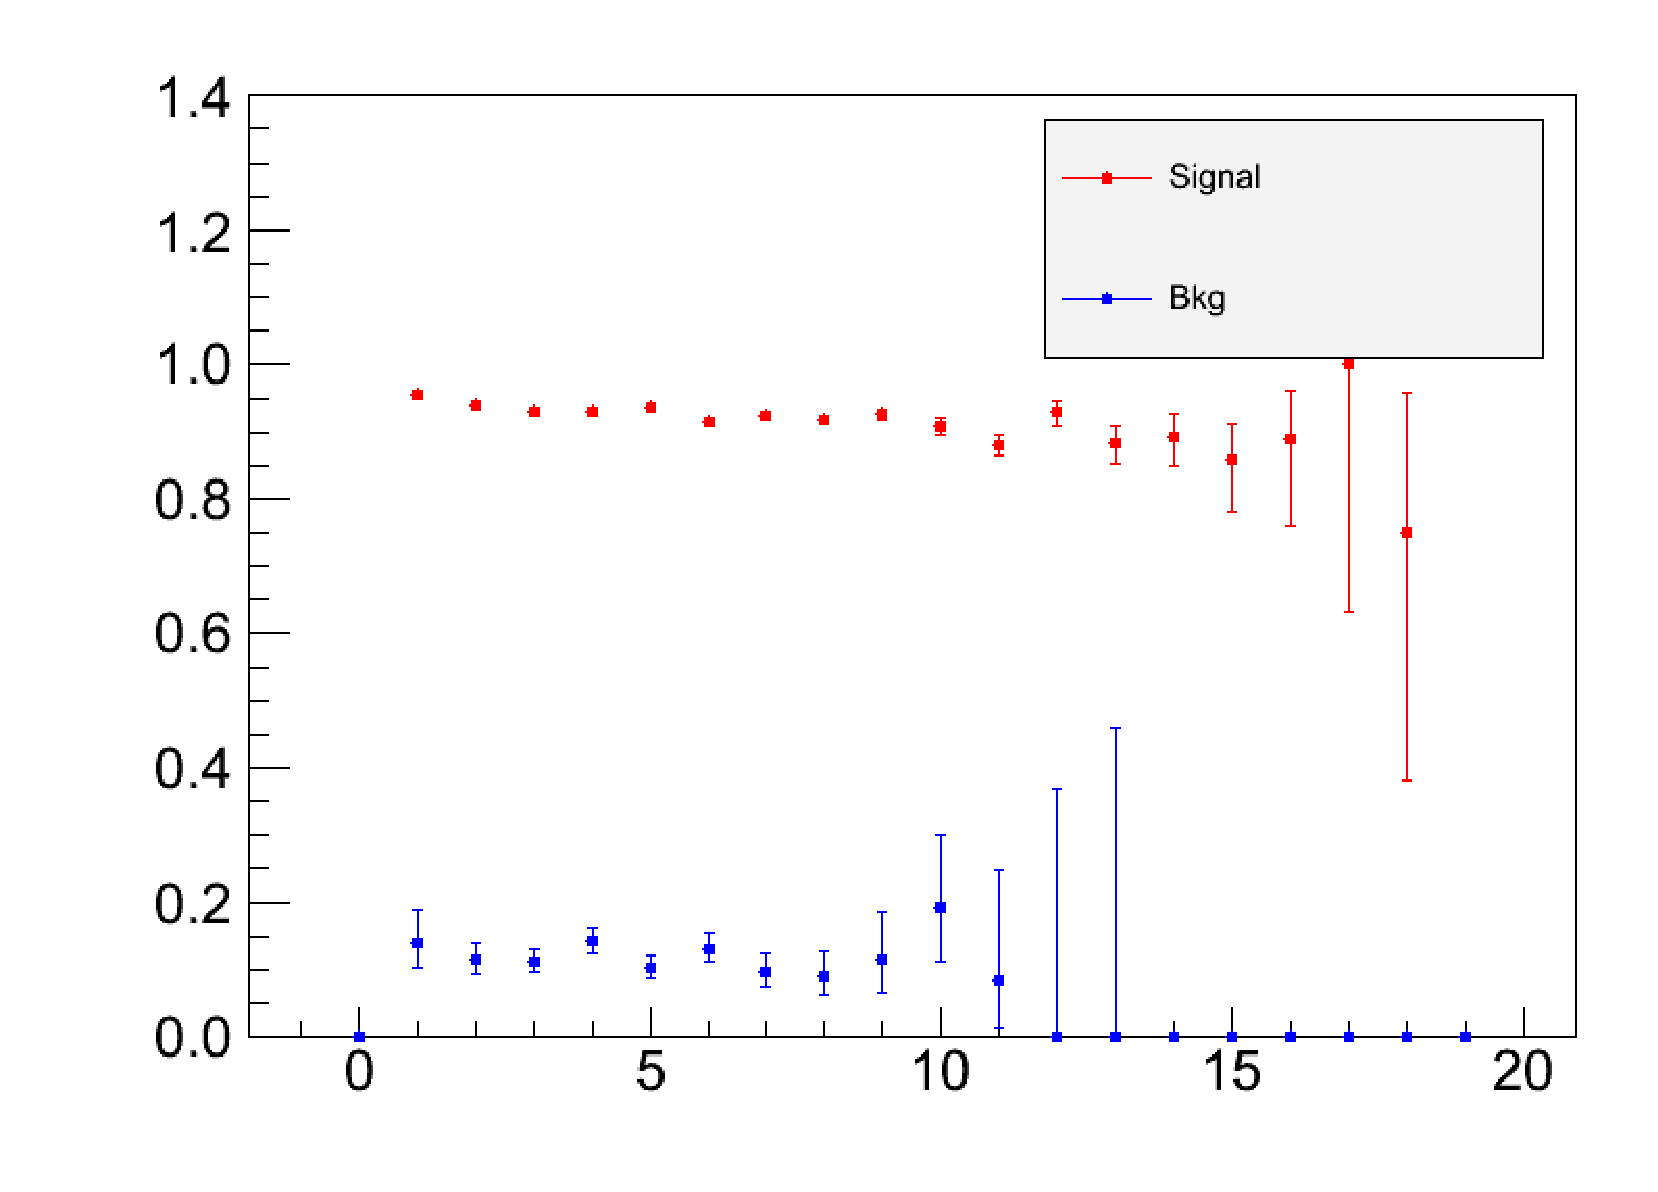
\includegraphics[width=0.48\textwidth]{figures/EleIsoEffVsNVtx_PFIso_Barrel_Pt20To30.pdf}}
\subfigure[Endcap]{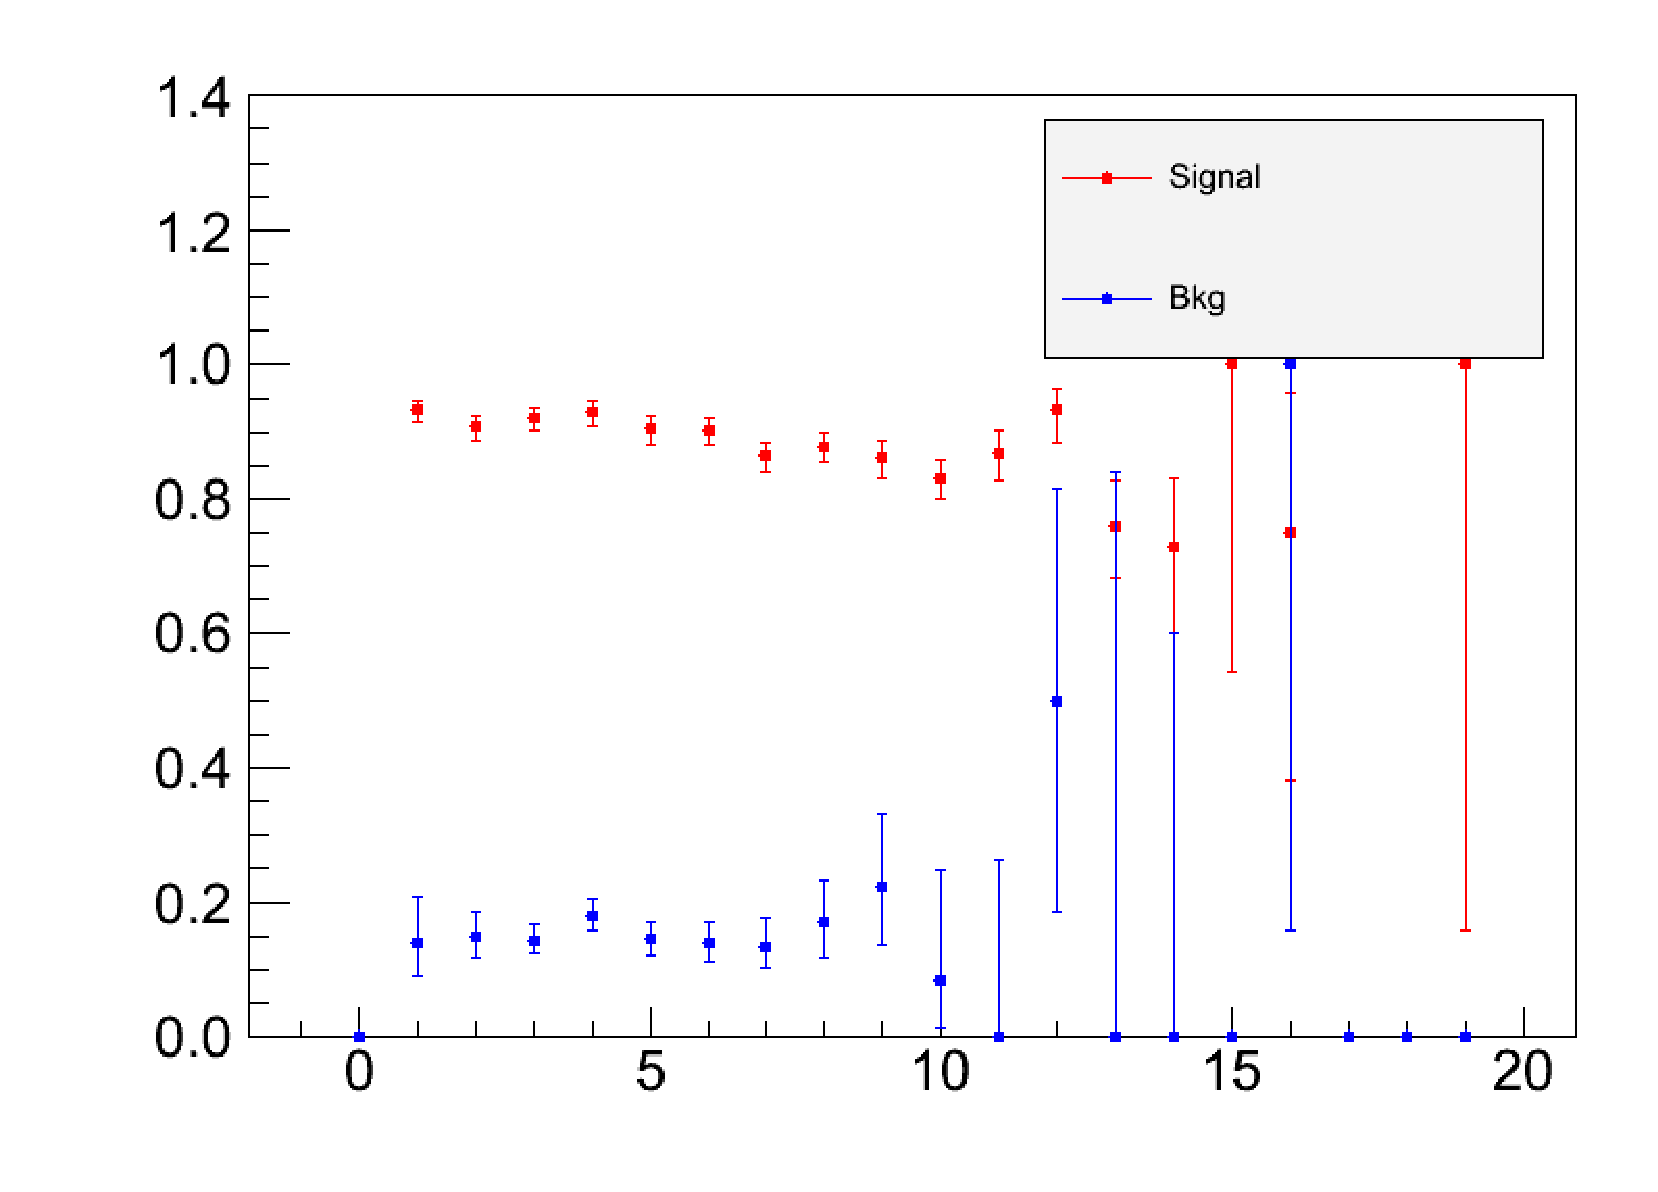
\includegraphics[width=0.48\textwidth]{figures/EleIsoEffVsNVtx_PFIso_Endcap_Pt20To30.pdf}}
\caption{The isolation efficiency of the particle flow isolation cut with the $1$GeV threshold on neutrals
for leptons with $p_{T}$ between $20$ and $30$ GeV in the HWW130 signal sample as a function of the 
number of reconstructed primary vertices, for barrel and endcap electrons.}
\label{fig:EleIsoEffVsNVtx_PFIso_Pt20To30}
\end{center}
\end{figure}




\begin{table}[!htbp]
\begin{center}
\begin{tabular}{|l|c|c|}
\hline
\multicolumn{3}{|c|}{Barrel} \\
\hline
Category                  & Std Iso Cut & PF Iso Cut \\
\hline
$p_{T}$ in $(10,15)$ GeV  &  $-22\%$    & $-10\%$    \\
$p_{T}$ in $(15,20)$ GeV  &  $-12\%$    & $-5\%$     \\
$p_{T}$ in $(20,30)$ GeV  &  $-10\%$    & $-2\%$     \\
\hline
\multicolumn{3}{|c|}{Endcap} \\
\hline
Category                  & Std Iso Cut & PF Iso Cut \\
\hline
$p_{T}$ in $(10,15)$ GeV  &  $-21\%$    & $-3\%$    \\
$p_{T}$ in $(15,20)$ GeV  &  $-6\%$    & $-1\%$     \\
$p_{T}$ in $(20,30)$ GeV  &  $-7\%$    & $-7\%$     \\

\hline
\end{tabular}
\caption{Comparison of the fractional loss of isolation efficiency for electrons from no 
pileup to a scenario with $10$ reconstructed primary vertices. }
\label{tab:EleIsoEfficiency_LossFromPileup_CompareStdWithPF}
\end{center}
\end{table}




\subsection{Summary}

To summarize the results of this extensive study, we observe a significant gain in performance
for particle flow isolation over the standard detector based isolation for electrons with $p_{T}<20$. 
This improvement is much larger for the barrel than for the endcap. We observe that vetoing
an $\eta$-strip of $0.025$ gives a gain in performance for low $p_{T}$ endcap electrons, and no
change in performance in any other electron category. As a result we choose to perform this 
$\eta$-strip veto. 

For high pileup scenarios, we observe a significant improvement by requiring a $\Delta$z $ < 0.1$cm
cut for charged particles. To control the effect of pileup we apply a $p_{T}$ threshold of $1$GeV
on neutral hadrons and particle flow photons inside the isolation cone, as the most simplistic
solution. It is observed that the efficiency loss with the amount of pileup is decreased by a factor of
two to three relative to the standard detector based isolation cut. 

Finally, we reserve the option to remove this threshold on neutral particles and applying an appropriate 
energy density based subtraction scheme for much more severe pileup scenarios in the future, where 
the simple threshold on neutrals will no longer be sufficiently effective.


